\documentclass[11pt]{article}
\usepackage[margin=1in]{geometry}
\usepackage{amsmath,amssymb,amsthm,mathtools}
\IfFileExists{lmodern.sty}{\usepackage{lmodern}}{}
\usepackage[expansion=false]{microtype}
\usepackage{booktabs,array,longtable,graphicx}
\usepackage{xurl}
\usepackage{enumitem}
\usepackage{xcolor}
\usepackage{tikz}
\usetikzlibrary{arrows.meta}
\usepackage[colorlinks=true,linkcolor=blue!50!black,citecolor=green!35!black,urlcolor=blue!50!black]{hyperref}
\usepackage[nameinlink]{cleveref}

\newtheorem{theorem}{Theorem}[section]
\newtheorem{proposition}[theorem]{Proposition}
\theoremstyle{definition}
\newtheorem{definition}[theorem]{Definition}
\theoremstyle{remark}
\newtheorem{remark}[theorem]{Remark}
\newcommand{\TV}{\operatorname{TV}}
\newcommand{\Cpl}{\operatorname{Cpl}}

\title{Empirical Site Separation:\\ Bending, Tearing, Contextuality and Holonomy\\ in a National Survey, Retrained Language Models\\ and Clinical Data}
\author{Vinay K. Awasthi\\
Department of Applied Mathematics and Statistics\\
Johns Hopkins University\thanks{Code and checks: \url{https://github.com/vkawasth/Trainingless-Transformer-NoGradientDescent/tree/main/monitor}.
\texttt{check\_monitor.py} recomputes or verifies every number reported here. All papers of the programme:
\url{https://github.com/vkawasth/Trainingless-Transformer-NoGradientDescent/tree/main/papers}.}}
\date{October 10, 2026, draft 4}

\begin{document}
\maketitle

\begin{abstract}
Language models are retrained, survey questions are reworded, clinical populations drift, and in each case the question is the same:
when the information changes, did the structure only bend, did it tear, did it break, and what changed that the summary numbers do not
show? We turn the programme's theory into a monitor and run it on GPT-3.5 and GPT-4 before and after their June 2023 update (eight
question sets, including medical licensing questions asked with intact and with damaged prompts), on the General Social Survey,
1985--2024, on two cycles of NHANES, and, in pre-registered analyses with replication samples, on intensive-care, hospital and
cardiology records and on two COVID-19 mental-health panels of up to six waves. On the survey we test the separation of sites of the programme: that contextuality (Layer 3),
the geometry of couplings (Layer 2) and the holonomy of operations (Layer 1) are different invariants. On $1320$ system-years of eleven
spending items in two randomized wordings, a contextuality test that assumes identical connections reports a contextual fraction of
$0.02$--$0.58$ in every one, while Contextuality-by-Default in canonical form absorbs all of it as direct influence: no item pair is
detected as contextual after combining its years and correcting for the $55$ pairs (the closest, crime and drugs, has $p=0.0073$
against a threshold of $0.0009$). The same wordings carry a
non-flat connection, a nonzero holonomy class in $H^1=\mathbb R^{10}$ in every one of the $24$ years, dominated by ``welfare'' against
``assistance to the poor''; and the items are often dependent, a nonzero distance from the entropy brane's intersection point ($1140$ of $2640$ tables at a
Bonferroni level).
The three invariants dissociate on the same systems, as the stratification of the programme requires, and no one scalar orders them. We draw the coupling polytopes of real margins as moment
polytopes of toric surfaces with their nonzero torus branes: the maximum-entropy coupling never carries one and the leximin coupling
always carries at least half of them, and the one decided survey tear is a toric blow-down at a fixed point, taking the $3\times3$
polytope from $15$ to $12$ vertices. Retraining tears are rank reversals of the two models; damaged prompts flip the correctness of $10$--$17\%$ of items while
moving accuracy by $1$--$5$ points. In the survey panels the answers of three waves do not compose, but a latent Markov chain seen
through unreliable answers is not rejected in any panel, and the order of a respondent's answers adds nothing to their association with the 2008
vote or party identification beyond which answers were given. A published behavioural experiment serves as a positive control: the
programme's cyclic criterion reproduces its contextuality exactly; a planted-data check of the canonical test used elsewhere shows that it
holds its size but detects only large contextuality at the sample sizes here, so its non-detections rule out large effects only. In
pre-registered analyses of open clinical and panel data, available-case tables of a selectively measured quantity are incompatible beyond
sampling (lactate in two independent ICU samples, HbA1c in $101{,}766$ diabetic encounters, attrition in the UK panel): measurement is not
at random with respect to the measured states. With four waves, a latent first-order Markov chain is not rejected in either COVID-19
panel, although the answers do not compose: composition failure in the answers is consistent with measurement error on a Markov latent
state, though at these sample sizes the test has limited power against longer memory. No category broke at the $1\%$ level. The algebraic backbone, which no public data can reach, is tested on
synthetic data with closed-form ground truth and planted failures. Kleisli composition, the three-level tower, its mixed distributive
law and the interchange of couplings with kernels behave exactly as stated, and every predicted failure appears at its predicted place
with its predicted size. The one exception is instructive: a random-instance check is blind to a planted failure. On real panels one theorem of the backbone, the interchange law, shows that banding inflates the composition failure: the monitor's null is $41$--$51\%$ too small, although the failure survives the correction.  A three-level tower fitted on PhysioNet is idle at its reliability level between random halves of one population, as it should be. Under a shift between units it cannot represent the shift as specified, and its own lifting certificate measures the gap. Its Fano tubes, the toric types of the predicted system, show this as a confidently wrong chamber. With a family of floors, a posterior over binary channels, the tower's reliability level earns its keep in every pre-registered shift between ICU unit types and harms nowhere. The geometry of GSS item pairs forecasts their next chamber change beyond the margins, while per-stay ICU systems are almost all broken and their geometry forecasts nothing. Selection models not built on the triangle cells fit the UK panel's attrition and fail for ICU lactate and diabetic HbA1c. The map from information to outcome is tested for context invariance as membership in a toric variety. Four of eleven GSS items, and ICU unit types, leave it, and the toric type of the answer $\times$ outcome system records where. Point polytopes at the boundary turn out to be mostly artefacts of zero counts: their geometry is recoverable from a posterior, but it does not forecast death. A tracker built on the family of coupling polytopes and their normal fans shows the approach to a wall before the one decided survey tear and in the physiology of ICU patients who die. In recursive training with known truth, the clearest sign of destroyed information is the contexts' steady departure from the invariance variety, which fresh data cap; three of five pre-registered predictions fail, and we report them. A decision layer on the same geometry turns sources of known reliability into auditable decisions, with a support threshold, the weakest link and a typed record of why a conclusion fails to glue. Support floors on cells preserve the toric geometry exactly, by a shift to reduced margins, and a new obstruction appears: families that glue, but not with the floor. The ambience is carried by the total category of a functor from contexts into posets: policies act as an idempotent comonad on each fibre, summarising by floors as an idempotent monad, and their failure to commute with transport is a computable oplax 2-cell. On real scientific claims (SciFact) with weak verifiers, the layer is right when it acts and its wrong acts stay within a conformal guarantee, but it rarely acts, and its margin ranks pairs worse than plain confidence. We explain why the other deeper layers are not yet activated by the data. We state
where the programme falls short and list every dataset used across its ten papers.
\end{abstract}

\tableofcontents

%=====================================================================
\section{The question}\label{sec:question}
%=====================================================================

When a model is retrained, a question is reworded or a population changes, what is usually reported is a summary: an accuracy, a share of
respondents, a prevalence. The programme of which this paper is part \cite{Bands,Bridges,Conditionals,Architecture} claims that
summaries miss the structure of the change. Two quantities measured on the same units define a coupling, the coupling lies in a polytope
fixed by the margins, and the polytope changes in three ways as the margins move: it bends within a chamber, it tears across a wall where
it changes combinatorial type, and it breaks at the boundary where a margin reaches zero \cite[Thm.~3.3]{Bands}. Over several contexts, the
same content measured differently may be contextual or merely directly influenced \cite[\S4]{Bridges}. And when the same units are seen
twice, the coupling of a content with itself across contexts can carry change the margins do not show.

This paper tests these claims on data where the information demonstrably changed:
\begin{itemize}[leftmargin=*,nosep]
\item \emph{retraining}: GPT-3.5 and GPT-4, March versus June 2023, on the same questions \cite{ChenZaharia2024}, and, for the medical
  questions, intact versus damaged prompts;
\item \emph{society}: the General Social Survey, where the wording of spending questions is randomized and where three-wave panels
  follow the same people \cite{GSS,Smith1987};
\item \emph{clinical}: two NHANES cycles, the medical licensing questions inside the retraining data, and, under plans written before
  the data were opened, two independent ICU samples, $101{,}766$ diabetic encounters and four heart-disease sites;
\item \emph{longitudinal}: the UK and Irish COVID-19 mental-health panels, with up to six waves on the same people;
\item \emph{a positive control}: a published behavioural experiment in which contextuality is known to be present;
\item \emph{the structural backbone}: synthetic data with closed-form ground truth and planted failures, for the monad of kernels, the
  three-level tower, its distributive law and the interchange law (\cref{sec:structure}).
\end{itemize}
None of these designs identifies the effect of a policy; the survey analyses describe how measured attitudes change, not why.

The survey also tests a structural claim of the programme. ThreeLayers \cite{ThreeLayers} organizes the theory in three layers, each with
its own invariant on its own site: the holonomy of operations (Layer~1), information on a site with a global joint (Layer~2), and
contextuality on a cover without one (Layer~3); each is nontrivial on its own site and zero on the others \cite[\S2]{ThreeLayers},
and for the coefficient systems of Layers~2 and~3 this is made precise by the non-unification and vanishing theorems
\cite[Thms.~15.1, 15.3]{ThreeLayers}. These are structural statements, not predictions about data. Its randomized wordings, its forty years of cross-sections and its panels let us compute all three
on the same respondents (\cref{sec:sites}), after checking on a published experiment that the test detects contextuality where it
exists (\cref{sec:positive}). \Cref{sec:clinical,sec:panels6} test the remaining claims, with plans fixed in advance and replication
samples, on clinical records and on six-wave panels. \Cref{sec:geometry} then draws the toric and Floer-theoretic picture of \cite{Bridges} for
margins taken from these data, and \cref{sec:datasets} lists the data of the whole programme.

%=====================================================================
\section{The monitor}\label{sec:monitor}
%=====================================================================

\begin{definition}[System]
A \emph{system} is a pair of contents $A,B$ with finitely many outcomes, measured jointly on the same units in each of several contexts.
In context $c$ the joint table $T_c$ has margins $(f_c,g_c)$. Contexts are versions of a model, prompts, wordings of a question, survey
years, panel waves or survey cycles.
\end{definition}

\paragraph{Bands.} Each margin is given an elementwise band: Wilson intervals at level $\alpha/k$ for $k$ outcomes, $\alpha=0.05$,
then tightened so that the band is consistent with total mass one \cite[Prop.~2.2]{Bands}. For weighted surveys the sample size is
Kish's effective size $(\sum w)^2/\sum w^2$ \cite{Kish1965}; clustering and stratification are not modelled.

\paragraph{Regime.} The walls of a pair of margins are the hyperplanes $f(I)=g(J)$; the tear margin $m_T$ is the distance to the
nearest wall and the break margin the smallest margin \cite[Thm.~3.2]{Bands}. A wall is \emph{decided} on a band when the range of
$f(I)-g(J)$ over the band excludes zero \cite[Prop.~3.4]{Bands}. A change $c\to c'$ is a
\begin{itemize}[leftmargin=*,nosep]
\item \emph{tear} if some wall decided in both states changes side;
\item \emph{possible tear} (tear?) if the point estimates change side of a wall that is undecided in at least one of the two states;
\item \emph{break} if an outcome whose band lies above $1\%$ in $c$ has its band below $1\%$ in $c'$;
\item \emph{bend} otherwise.
\end{itemize}
The \emph{stress} of the change is $s=\bigl(\TV(f_c,f_{c'})+\TV(g_c,g_{c'})\bigr)/m_T(f_c,g_c)$.

\begin{proposition}[Tears need stress]\label{prop:stress}
If the point estimates of a change cross a wall, then $s\ge1$.
\end{proposition}
\begin{proof}
The segment from $(f_c,g_c)$ to $(f_{c'},g_{c'})$ meets the wall, every point of the wall is at distance at least $m_T(f_c,g_c)$ from
$(f_c,g_c)$ in the metric $\TV+\TV$ \cite[Thm.~3.2]{Bands}, and the distance from $(f_c,g_c)$ to the crossing point is at most the
length of the segment, which is the realized change.
\end{proof}

So stress below one certifies a bend; stress above one is necessary but not sufficient for a tear. Since every tear has stress at least
one by the proposition, the stresses reported below carry information only through their size.

\begin{remark}[Near-empty categories]\label{rem:empty}
When an outcome is nearly empty in both contents (a model almost never fails to answer), the wall comparing the two small shares is very
close, $m_T$ is tiny and the stress is large even for a small change. Such walls are never decided on the bands, so they produce possible
tears, not tears; we flag them where they occur.
\end{remark}

\paragraph{Context.} We test Contextuality-by-Default in its canonical form \cite{DzhafarovCervantesKujala2017}: each content is replaced
by all its dichotomizations (for three outcomes, each outcome against the other two), and the system is noncontextual exactly when some
coupling of $(A_1,B_1,A_2,B_2)$ reproduces the two context tables and couples every dichotomization of $A$, and of $B$, maximally with
itself across the two contexts. This is a linear program; its \emph{deficit}, the maximal minus the attainable total agreement of the split
connections, is positive exactly when the system is contextual. For binary contents it reduces to the cyclic system of rank $2$
\cite{DzhafarovKujala2016,KujalaDzhafarov2016}, contextual exactly when $\lvert\langle A_1B_1\rangle-\langle A_2B_2\rangle\rvert>\Delta$ with
$\Delta=\lvert\langle A_1\rangle-\langle A_2\rangle\rvert+\lvert\langle B_1\rangle-\langle B_2\rangle\rvert$ the direct influence of the context on
the contents; we also report this rank-$2$ statistic for the dichotomization ``first outcome against the rest'', computed both by the
criterion and by the linear program of \cite[\S4]{Bridges}, which agree on every case. A three-outcome system can be contextual in its
splits while this single dichotomization is not, and the code's unit tests show it happens often (219 of 400 random systems that are
noncontextual in the single dichotomization are contextual in the canonical form).

\paragraph{Churn.} When the same units are observed in two contexts, the coupling of a content with itself across them is observed, not
assumed. Its agreement $P(X=Y)$ is at most $\sum_i\min(f_i,g_i)$, the agreement of the maximal coupling that Contextuality-by-Default
assigns to a connection.

\begin{proposition}[Excess churn and masked change]\label{prop:churn}
The \emph{excess churn} $\sum_i\min(f_i,g_i)-P(X=Y)$ is nonnegative, and zero exactly when the observed coupling is a maximal coupling. For a
binary outcome with $1$ meaning correct, let $\ell=P(X=1,Y=0)$ be the mass lost and $\gamma=P(X=0,Y=1)$ the mass gained, both as shares of
all units. Then the excess churn is $2\min(\ell,\gamma)$: twice the \emph{masked} change, the losses that are offset by gains and so
invisible in the net change $\gamma-\ell$.
\end{proposition}
\begin{proof}
A coupling puts at most $\min(f_i,g_i)$ on each diagonal cell, with equality on all of them exactly for a maximal coupling. For two outcomes,
$\sum_i\min(f_i,g_i)=1-\lvert\gamma-\ell\rvert$ and $P(X=Y)=1-\ell-\gamma$, whose difference is $\ell+\gamma-\lvert\gamma-\ell\rvert=2\min(\ell,\gamma)$.
\end{proof}
\noindent The lost mass $\ell$ is what the model-update literature calls the rate of \emph{negative flips} \cite{Yan2021}; the proposition
says that the part of it that the net accuracy hides is exactly half the distance of the observed coupling from the maximal one.
Excess churn mixes real change with measurement noise: a model sampled at positive temperature, or a respondent answering a survey twice,
disagrees with itself. It is an upper bound on masked change until a noise floor is subtracted, and none of the data here contain true
replicates.

\paragraph{Composition.} For three waves on the same units, the gluing gap $I(X_1;X_3\mid X_2)$ vanishes exactly when the joint law of the
three waves is the gluing of the first two waves with the last two \cite[Prop.~4.8]{Bands}, that is, when the answers form a Markov chain.
A positive gap does \emph{not} by itself mean that the underlying change fails to compose: a stable attitude measured with independent
error at each wave also gives a positive gap \cite{Converse1964,Achen1975,WileyWiley1970}. We therefore test the observed answers
against the glued (Markov) law, by resampling from it, and fit three latent-class models with three classes, by EM from $30$ starts:
\emph{stable} (a fixed latent class answered with the same response law at every wave; $8$ parameters), \emph{drifting} (a fixed class with
a response law for each wave; $20$ parameters) and \emph{latent Markov} (the class follows a Markov chain over the waves, answered with one
response law; $20$ parameters) \cite{Wiggins1973}. Each is tested by the likelihood ratio $G^2$ against the saturated table, on $18$, $6$
and $6$ degrees of freedom. The latent Markov model is the gluing of the programme one level down: if it fits, the attitudes may compose
while the answers do not. The gap is a plug-in estimate, biased upward by about $0.014$ bits at $n\approx600$; the Markov null carries the
same bias.

%=====================================================================
\section{Data}\label{sec:data}
%=====================================================================

\paragraph{Retraining.} The LLM-drift data of Chen, Zaharia and Zou \cite{ChenZaharia2024} contain the answers of GPT-3.5 (versions 0301 and
0613) and GPT-4 (0314 and 0613) to the same questions in eight tasks, at temperature $0.1$. Each answer is coded \emph{correct},
\emph{wrong} or \emph{no valid answer}, using the last stated answer (``the answer is (X)'', the last bracketed yes or no, the last boxed
number). For the sensitive questions the outcome is answered or refused, for LeetCode directly usable code or not, and for OpinionQA,
which has no correct answer, answered (a valid option) or not. The USMLE file asks each of its $340$ questions twice: once with the intact
prompt and once with a damaged one, in which a stretch of text is deleted: a passage of the question stem in $89\%$ of the questions,
option (A) in $10\%$; two pairs are identical. We use the intact prompts for the update and treat intact versus damaged as a second change of information.
Pooling both prompts reproduces the published GPT-4 accuracy, $86.6\%\to82.1\%$; our figures for primes ($84.0\%\to51.1\%$) and for its
response rate to sensitive questions ($21\%\to5\%$) also match. A task's system has contents $A$ = GPT-3.5 and $B$ = GPT-4, measured on
the same items, and contexts March and June.

\paragraph{Society.} The General Social Survey \cite{GSS}, read through the \texttt{gssr} package \cite{Healy2024}, asks whether the
government spends too little, about the right amount or too much on a list of items, each in one of two randomly assigned wordings: $X$
(``welfare'', ``solving the problems of the big cities'', ``improving the conditions of Blacks'', \dots) and $Y$ (``assistance to the poor'',
``assistance to big cities'', ``assistance to blacks'', \dots) \cite{Smith1987,HuberParis2013}. No respondent gets both wordings of an item.
We use three pairs of items, 1985--2024, with the weight \texttt{wtssps}, and in \cref{sec:sites} all eleven items asked in both wordings. A system has two items as contents and the wordings, or the
years, as contexts. The 2006--2010, 2008--2012 and 2010--2014 panels follow the same respondents through three waves and record their 2008
presidential vote; we use the respondents who answered the welfare item in the same wording in all three waves, unweighted.

\paragraph{Clinical.} NHANES 2009--2010 and 2011--2012 \cite{NHANESpkg}, adults $20+$ with exam weights: contents diabetes (self-reported
diagnosis) and BMI class (below 25, 25--30, 30 and above); contexts the two cycles. The medical licensing questions (USMLE) in the
retraining data are the second clinical system. Open, de-identified hospital data are used in \cref{sec:clinical}; the credentialed
electronic health records of MIMIC-IV \cite{MIMICIV} are not, because their data use agreement does not allow them to leave the
credentialed user's machine. The protocol of \cite[\S11]{Bands} for them is provided as a kit to be run locally.

\paragraph{Open clinical and longitudinal data.} PhysioNet 2012 ICU stays (sets A and B) \cite{Silva2012,Goldberger2000}, the UCI
Diabetes 130-US Hospitals \cite{Strack2014,UCIDiabetes} and Heart Disease \cite{Detrano1989,UCIHeart} data, and the UK and Irish strands of
the C19PRC panels \cite{McBride2021,SpikolIE} are described with their analyses in \cref{sec:clinical,sec:panels6}; the Snow Queen tables
\cite{CervantesDzhafarov2018} in \cref{sec:positive}; the synthetic data of the structural tests in \cref{sec:structure}.

%=====================================================================
\section{Retraining}\label{sec:llm}
%=====================================================================

\begin{table}[ht]
\centering\footnotesize\setlength{\tabcolsep}{3.5pt}
\caption{GPT-3.5 and GPT-4, March $\to$ June 2023 (USMLE: intact prompts). Accuracy (OpinionQA, sensitive questions: response rate) in
percent. Regime and stress of the system (GPT-3.5, GPT-4) from March to June. $s/\Delta$: the rank-$2$ Contextuality-by-Default statistic
for correct against not, against the direct influences; the canonical test (all dichotomizations of the three outcomes) is noncontextual in
every task as well. Lost/masked: percent of all items correct in March and not in June, and the part of it offset by gains
(\cref{prop:churn}).}\label{tab:llm}
\begin{tabular}{lrcccrccc}
\toprule
task & items & GPT-3.5 & GPT-4 & regime & stress & $s/\Delta$ & \multicolumn{2}{c}{lost/masked}\\
 & & & & & & & GPT-3.5 & GPT-4\\
\midrule
USMLE (medical) & 340 & 63.5$\to$65.0 & 88.2$\to$84.7 & tear? & 19.0 & 0.01/0.10 & 7.6/7.6 & 4.7/1.2\\
OpinionQA & 1506 & 100.0$\to$100.0 & 97.9$\to$24.7 & bend & 35.6 & 1.46/1.46 & 0.0/0.0 & 73.3/0.1\\
sensitive questions & 100 & 2.0$\to$8.0 & 21.0$\to$5.0 & tear? & 1.2 & 0.28/0.44 & 0.0/0.0 & 16.0/0.0\\
primes & 1000 & 52.9$\to$76.0 & 84.0$\to$51.1 & tear & 152.8 & 0.00/1.12 & 17.3/17.3 & 47.6/14.7\\
happy numbers & 500 & 30.6$\to$48.2 & 83.6$\to$35.2 & tear & 25.8 & 0.22/1.32 & 14.0/14.0 & 53.8/5.4\\
ARC & 467 & 10.9$\to$14.1 & 24.4$\to$27.0 & bend & 27.0 & 0.04/0.12 & 1.7/1.7 & 3.2/3.2\\
LeetCode (easy) & 50 & 22.0$\to$2.0 & 52.0$\to$10.0 & bend & 2.4 & 0.52/1.24 & 20.0/0.0 & 46.0/4.0\\
HotpotQA (agent) & 7405 & 22.3$\to$13.8 & 1.2$\to$37.0 & tear & 12.7 & 0.11/0.89 & 12.7/4.2 & 0.4/0.4\\
\bottomrule

\end{tabular}
\end{table}

\emph{Tears are reversals.} Three changes are tears decided on the bands: primes, happy numbers and HotpotQA, and in all three GPT-3.5 and
GPT-4 trade places. On primes and happy numbers the wall crossed first is $f_{\mathrm{correct}}=g_{\mathrm{correct}}$: GPT-3.5 rises from
$52.9\%$ to $76.0\%$ on primes while GPT-4 falls from $84.0\%$ to $51.1\%$. On HotpotQA the order reverses the other way. The sensitive
questions give a possible tear, with stress $1.2$; there too the two models trade places (GPT-3.5 answers $2\%\to8\%$, GPT-4
$21\%\to5\%$), but $100$ questions do not decide the wall. USMLE is a possible tear of the kind of \cref{rem:empty}: the wall crossed
compares the two models' shares of invalid answers, both below $1\%$, and the stress of $19$ reflects that wall's closeness, not the size of
the change.

\emph{A degenerate system.} OpinionQA is the largest change in the data, GPT-4's response rate falling from $97.9\%$ to $24.7\%$, and the
monitor calls it a bend. That is correct and instructive: GPT-3.5 answers every question in both months, so its margin is a vertex, the
coupling polytope is a single point in both months, and no change of GPT-4's margin can tear it. A system with one content at a vertex has
no structure to tear; the change must be read from the other content's margin.

\emph{The change is direct influence, not contextuality.} In every task $s\le\Delta$, and the canonical test finds no contextuality either.
Apart from OpinionQA, where GPT-3.5 is constant and $s=\Delta$ identically, the margins $\Delta-s$ range from $0.08$ (ARC) to $1.1$ (primes
and happy numbers). The update changed each model's distribution of answers, and that direct influence accounts for the joint tables of
the two models.

\emph{Masked change.} On intact USMLE prompts GPT-4 lost $4.7\%$ of all items ($5.3\%$ of the items it had right in March) and regained
$1.2\%$, so its net drop of $3.5$ points hides little; GPT-3.5's gains ($9.1\%$) more than offset its losses ($7.6\%$), all of them masked.
On primes GPT-3.5 improved by $23$ points and still lost $17.3\%$ of all items, a third of its March correct answers. Without replicate
answers these are upper bounds on masked damage: decoding noise at temperature $0.1$ cannot be separated from them.

\begin{table}[ht]
\centering\footnotesize
\caption{USMLE, intact versus damaged prompt, same $340$ questions; differences are computed before rounding. Accuracy in percent; lost and gained: percent of all questions whose
correctness changes from intact to damaged; excess churn (\cref{prop:churn}). The intervals are paired bootstraps over questions
(4000 resamples).}\label{tab:usmle}
\begin{tabular}{llccccc}
\toprule
model & version & intact & damaged & lost & gained & excess churn\\
\midrule
GPT-3.5 & March & 63.5 & 62.4 & 7.1 & 5.9 & 0.118\\
GPT-3.5 & June & 65.0 & 60.6 & 10.6 & 6.2 & 0.124\\
\multicolumn{7}{r}{\emph{GPT-3.5: change of the damage cost, June minus March: +3.2 points, 95\% interval [-1.5, +8.2]}}\\
GPT-4 & March & 88.2 & 85.0 & 6.8 & 3.5 & 0.071\\
GPT-4 & June & 84.7 & 79.4 & 8.5 & 3.2 & 0.065\\
\multicolumn{7}{r}{\emph{GPT-4: change of the damage cost, June minus March: +2.1 points, 95\% interval [-1.5, +5.6]}}\\
\bottomrule

\end{tabular}
\end{table}

\emph{Damaged information.} \Cref{tab:usmle} changes the information instead of the model. Damaging the prompt costs between $1.1$ and $5.3$
points of accuracy, but it changes the correctness of $10$--$17\%$ of the questions: most of the item-level change is masked in the
accuracy. Both models lose more to the damaged prompt in June than in March (GPT-4 $3.2\to5.3$ points, GPT-3.5 $1.1\to4.4$), which would
mean that the update made them more fragile to damaged information; but the paired intervals include zero, so these data do not establish it.

\emph{Breaking.} No outcome fell below the $1\%$ band, so no change is a break at that level. The nearest case is GPT-4's ``no valid answer''
on happy numbers, $9.4\%$ in March and exactly $0$ in June: the category emptied, but with $500$ items the upper band is $1.1\%$.

%=====================================================================
\section{Society}\label{sec:gss}
%=====================================================================

\begin{table}[ht]
\centering\footnotesize\setlength{\tabcolsep}{4pt}
\caption{GSS spending items, 1985--2024. Direct influence of the wording: median absolute change of the share ``too little'', in points.
Contextual: years in which the point estimates are contextual, for the rank-$2$ test on ``too little'' against the rest and for the
canonical test on all dichotomizations. Posterior: the largest posterior probability of canonical contextuality over the years
(Dirichlet posteriors at the effective sample sizes, $1000$ draws). Regimes of the year-to-year changes in each wording: bend / tear? /
tear / break.}\label{tab:gss}
\begin{tabular}{lcccccc}
\toprule
items & direct $A$ & direct $B$ & contextual (rank 2 / canonical) & posterior & wording $X$ & wording $Y$\\
\midrule
welfare-cities & 43.9 & 26.8 & 0 / 0 / 0 & 0.06 / 0.00 & 10/13/0/0 & 12/11/0/0\\
welfare-race & 44.7 & 6.5 & 0 / 2 / 0 & 0.80 / 0.00 & 9/14/0/0 & 8/14/1/0\\
health-education & 1.6 & 3.6 & 3 / 10 / 8 & 0.97 / 0.93 & 6/17/0/0 & 9/14/0/0\\
\bottomrule

\end{tabular}
\end{table}

\emph{Wording is a direct influence.} Calling welfare ``assistance to the poor'' raises the share saying ``too little'' by a median of
$44$--$45$ points, the classic GSS wording effect \cite{Smith1987}, and calling the cities item ``assistance to big cities'' changes it by
$27$. Welfare and cities is noncontextual in every year under both tests. Welfare and race is contextual at the point estimates in two years
of the canonical test (posterior probability $0.80$ at most). Health and education is the one candidate: contextual at the point estimates
in $3$ of $24$ years for the rank-$2$ test and in $10$ of $24$ for the canonical one, with posterior probabilities between $0.37$ and
$0.97$ in those years. Only 1988 exceeds $0.95$ ($0.968$), and none comes near the screen $1-0.05/72\approx0.9993$ for $72$
system-years (with $1000$ draws, passing it would require every draw to be contextual). This posterior screen is not a corrected test,
and it is optimistic, since it ignores the clustered design. The answer scale is ordered, so we repeated the canonical test with only the
two order-respecting cuts (``too little'' against the rest, ``too much'' against the rest): the welfare and race flags disappear, since
they come from the split ``about right'' against the two extremes, and health and education keeps $8$ of its $10$ flags, with posterior
probabilities at most $0.93$. We conclude that wording acts as a direct influence everywhere, and that the health and education system lies
close to the contextuality boundary in many years without crossing it decidedly in any. Whether the two wordings measure the same content
at all is debated \cite{HuberParis2013}; the Contextuality-by-Default reading is agnostic about it.

\emph{Tears over four decades.} Most year-to-year changes bend or possibly tear: the point estimates of two items often sit near a wall, so
small changes cross it without the bands deciding. One tear is decided: for welfare and race in wording $Y$, from 2014 to 2016, the wall
$f_{\mathrm{too\ little}}=g_{\mathrm{about\ right}}+g_{\mathrm{too\ much}}$ is crossed, that is $f_1+g_1$ passes $1$. In 2014 ``too little'' for
``assistance to the poor'' ($62.5\%$) and for ``assistance to blacks'' ($26.9\%$) add to $0.89$; in 2016 they add to $1.13$. After the tear the
margins force at least $13\%$ of respondents to say ``too little'' to both: a combination that could previously be absent no longer can be.
The bands are simultaneous within a state but not across the $138$ year-to-year steps; with a Bonferroni correction over the steps this tear
is only a possible tear. The step from 2018 to 2021, across the survey's move to the web, is among the three largest changes in three of
six series, but it spans three years and is not among the three largest per year in any.

\begin{table}[ht]
\centering\scriptsize\setlength{\tabcolsep}{3pt}
\caption{GSS panels, welfare item in each wording (``welfare'', ``assistance to the poor''). Agreement of the same respondent's answer
in waves 1 and 2, the maximal agreement the margins allow, the excess churn; the gluing gap of the three waves in bits (plug-in) with a
bootstrap interval, against the $95$th percentile of the gap under the glued (Markov) law of the answers ($400$ resamples, none of which
reaches the observed gap).}\label{tab:panels}
\begin{tabular}{llcccccc}
\toprule
panel & wording & $n$ & agree & max & excess & gluing gap [95\%] & Markov null $95\%$\\
\midrule
2006--2010 & welfare & 592 & 0.623 & 0.958 & 0.334 & 0.066 [0.047, 0.129] & 0.027\\
2006--2010 & the poor & 605 & 0.744 & 0.950 & 0.207 & 0.063 [0.047, 0.118] & 0.028\\
2008--2012 & welfare & 552 & 0.623 & 0.953 & 0.330 & 0.067 [0.049, 0.126] & 0.030\\
2008--2012 & the poor & 641 & 0.702 & 0.942 & 0.240 & 0.069 [0.051, 0.124] & 0.024\\
2010--2014 & welfare & 604 & 0.621 & 0.939 & 0.318 & 0.082 [0.060, 0.143] & 0.026\\
2010--2014 & the poor & 622 & 0.664 & 0.958 & 0.294 & 0.055 [0.043, 0.106] & 0.025\\
\bottomrule

\end{tabular}
\end{table}

\emph{Churn and composition.} The panels (\cref{tab:panels}) show the largest masked change in the paper. Between waves the margins of the
welfare item barely move, so a maximal coupling would let $94$--$96\%$ of respondents keep their answer; in fact $62$--$74\%$ do. A fifth to a
third of the respondents change their answer beyond what the shift of the margins requires. The answers of the three waves are not
glued: the gap of $0.055$--$0.082$ bits lies above every resample of the Markov law of the answers.

\begin{table}[ht]
\centering\scriptsize\setlength{\tabcolsep}{3pt}
\caption{Latent-class models of the panels (three classes): likelihood-ratio $G^2$ against the saturated table with its chi-square
$p$-value, and the gluing gap of the answers that the fitted model implies. Stable: $18$ degrees of freedom; drifting and latent Markov: $6$.
Parametric-bootstrap $p$-values ($100$ draws) give the same verdicts.}\label{tab:panelmodels}
\begin{tabular}{llcccccccc}
\toprule
 & & & observed & \multicolumn{2}{c}{stable} & \multicolumn{2}{c}{drifting} & \multicolumn{2}{c}{latent Markov}\\
panel & wording & $n$ & gap & $G^2$ ($p$) & gap & $G^2$ ($p$) & gap & $G^2$ ($p$) & gap\\
\midrule
2006--2010 & welfare & 592 & 0.066 & 32.3 (0.020) & 0.104 & 5.8 (0.442) & 0.059 & 5.9 (0.439) & 0.058\\
2006--2010 & the poor & 605 & 0.063 & 77.7 ($<0.001$) & 0.081 & 6.6 (0.364) & 0.055 & 9.5 (0.146) & 0.041\\
2008--2012 & welfare & 552 & 0.067 & 36.2 (0.007) & 0.105 & 6.7 (0.354) & 0.060 & 7.8 (0.256) & 0.052\\
2008--2012 & the poor & 641 & 0.069 & 35.8 (0.008) & 0.082 & 5.5 (0.480) & 0.065 & 7.1 (0.313) & 0.053\\
2010--2014 & welfare & 604 & 0.082 & 25.9 (0.103) & 0.094 & 2.9 (0.822) & 0.079 & 8.8 (0.188) & 0.053\\
2010--2014 & the poor & 622 & 0.055 & 18.0 (0.457) & 0.067 & 2.8 (0.836) & 0.053 & 4.5 (0.616) & 0.042\\
\bottomrule

\end{tabular}
\end{table}

\emph{Change or unreliability?} Unreliable answers around a fixed attitude also produce such a gap: the fitted stable models imply gaps
of $0.067$--$0.105$ bits (\cref{tab:panelmodels}). The stable model is rejected in the 2006 and 2008 panels for both wordings
($p\le0.02$) and not in the 2010 panel ($p=0.10$ and $0.46$); but it forces the answer margins to be equal at all waves, and they drift.
Both twenty-parameter models fit all six series ($p\ge0.15$): a fixed latent partition whose answers drift, and a latent Markov chain
answered with one response law. The panels therefore do not show that attitudes fail to compose. They are consistent with attitudes that
change as a Markov chain, which glues, seen through answers that are unreliable, which do not. The gluing gap of the answers measures the
unreliability as much as the change; three waves of about $600$ respondents cannot separate the drifting from the latent Markov reading.

\emph{Outcome.} The 2008 vote is associated with the first-wave answer, in both wordings: among those saying ``too little'' for welfare
$80.6$--$81.4\%$ voted for Obama, against $38.1$--$47.4\%$ of those saying ``too much''; for ``assistance to the poor'' the shares are
$68.6$--$75.0\%$ and $21.3$--$31.9\%$ (unweighted, panels of 2006, 2008, 2010). In the 2010 panel the vote preceded the first wave, so
this is an association, not a prediction.

%=====================================================================
\section{Site separation on the General Social Survey}\label{sec:sites}
%=====================================================================

ThreeLayers \cite[\S2]{ThreeLayers} assigns to each layer of the programme its own invariant, and its stratification remark states that each is
nontrivial on its own site and zero on the others (for Layers~2 and~3 in the precise form of \cite[Thms.~15.1, 15.3]{ThreeLayers}): Layer~1 (operations) carries a holonomy class $[g]\in H^1(\Gamma,A)$ of a connection on a
graph; Layer~2 (probability) lives on a site with a global joint, where the invariant is information, $I=\delta_tH$; Layer~3 (outcomes)
lives on a cover with no global context, where the invariant is a contextuality class and its contextual fraction. The theorems
concern sites and coefficients and predict nothing about data; what the survey can show is that the three invariants, computed on the
same respondents, are nonzero or zero independently of one another, which is what the stratification requires of them. We use all eleven national-spending items that the GSS asks in both randomized wordings
(welfare / the poor, big cities, Blacks, crime / law enforcement, drug addiction / rehabilitation, education, health, environment, space,
defense, foreign aid), every year 1985--2024: $55$ item pairs in $24$ years, $1320$ system-years. Between $54.6\%$ and $73.5\%$ say
``too little'' for ``assistance to the poor'' and between $13.4\%$ and $33.4\%$ for ``welfare'' (weighted, by year); $55{,}169$
respondents answered one of the two welfare wordings ($27{,}047$ and $28{,}122$), none both.

\subsection{Layer 3: contextuality is absorbed by direct influence}

\begin{figure}[!htbp]
\centering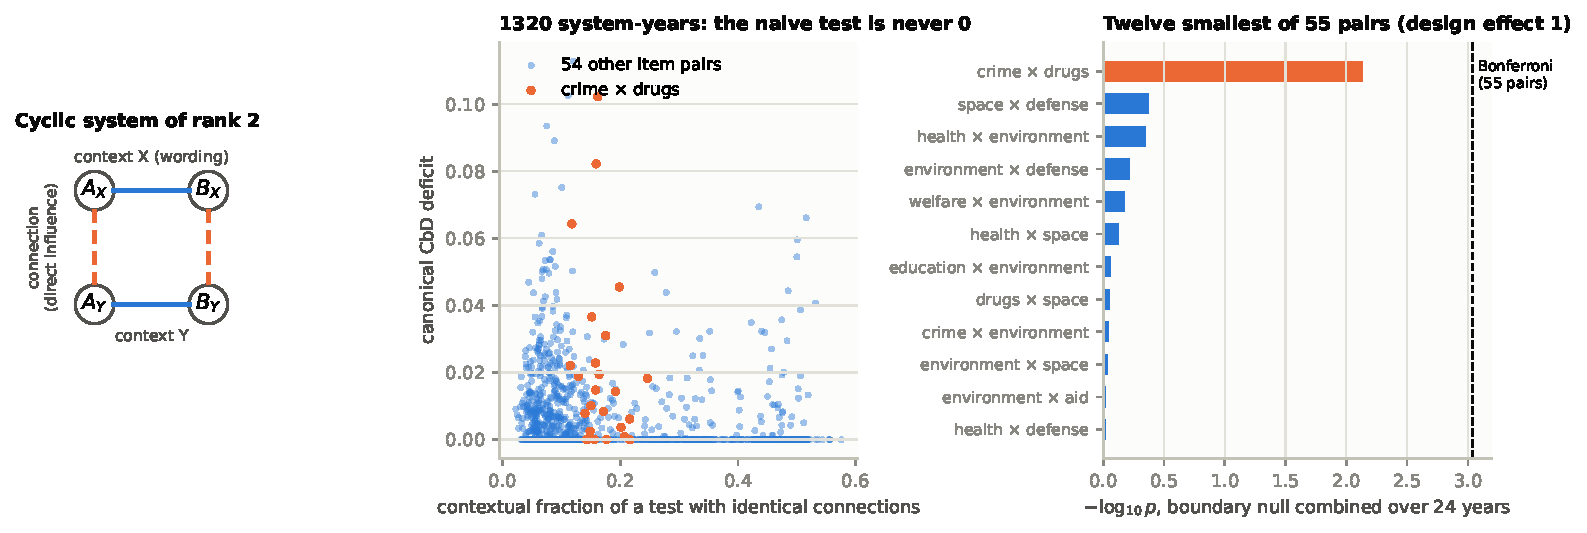
\includegraphics[width=\linewidth]{figs/fig_cbd.pdf}
\caption{Left: the system of two items in two wordings as a cyclic system of rank $2$; solid edges are contexts, dashed edges are
connections. Middle: for every system-year, the contextual fraction a test with identical connections would report, against the
canonical CbD deficit. Right: the twelve item pairs with the smallest combined $p$-values for canonical contextuality (boundary null,
Fisher over the $24$ years, design effect $1$); the dashed line is the Bonferroni threshold over $55$ pairs.}\label{fig:cbd}
\end{figure}

A test that treats the two wordings as the same measurement, as a Bell-type or Kochen--Specker test does, asks for one law $q$ of
$(A,B)$ under both tables. The noncontextual-fraction linear program of \cite{AbramskyBarbosaMansfield2017}, applied formally to this
model (which, having two different laws on one context, is outside the no-signalling setting for which that fraction is defined), gives $1-\max\{\lambda:\lambda q\le T_X,\ \lambda q\le T_Y\}
=\TV(T_X,T_Y)$, positive whenever the wording changes anything. It is positive in all $1320$ system-years, from $0.022$ to $0.576$
(median $0.119$; \cref{fig:cbd}). Contextuality-by-Default instead couples each item with itself across wordings maximally and asks
whether the rest fits. In canonical form the point estimates are contextual in $523$ system-years ($307$ with only the order-respecting
cuts, $93$ in the rank-$2$ reduction): the canonical test is far more sensitive than the binary one. To decide which flags are sampling
noise we test each against a noncontextual truth on the boundary: the Y table is moved toward the X table until the deficit vanishes,
both tables are simulated there at the effective sample sizes, and the $p$-value is the share of simulated deficits at least the observed
one ($200$ simulations per system-year; $p$-values of the form $(k+1)/201$ and $p=1$ for a zero deficit, so Fisher's combination below is
conservative). Combining the $24$ independent yearly samples of each pair by Fisher's method, the smallest $p$-value is $0.0073$ ($0.0041$
with $500$ simulations), for crime and drugs, which is flagged at
the point estimates in $20$ of $24$ years; the next is $0.42$. With design effect $2$ it is $0.15$. No pair passes the Bonferroni threshold
$0.05/55$. (The Dirichlet posterior used in \cref{sec:gss} is more liberal here: it puts $25$ system-years above $0.95$, because the
posterior of a statistic that is zero on a whole region piles up on the contextual side near the boundary.)

So the expectation that contextuality vanishes once direct influence is accounted for is borne out on the whole survey: the naive
test reports contextuality everywhere, and none is detected once direct influence is allowed. Non-detection is not proof of absence: the
boundary null is one natural noncontextual truth, not a proved least favorable one, and $523$ point estimates are contextual. Crime and drugs is the one system that sits persistently near the
boundary: in wording $X$ (``halting the rising crime rate'', ``dealing with drug addiction'') the two items are more strongly associated
than the shift of their margins alone allows when they are reworded as ``law enforcement'' and ``drug rehabilitation''. This is a
candidate for a designed test, not a finding.

\subsection{A positive control, and the power of the test}\label{sec:positive}

A negative result means little unless the test is shown to detect contextuality where it is known to be present. Cervantes and
Dzhafarov's Snow Queen experiment \cite{CervantesDzhafarov2018} is the standard behavioural case. It is a cyclic system of rank~$4$ in the
Bell design: two choices of character, each paired with two choices of characteristic, $1{,}799$ respondents, one context each. Its
direct influences are large, yet the authors find contextuality beyond them. We recomputed it from the published proportions and sample
sizes with the programme's code, both the closed-form criterion and the linear program of \cite[\S4]{Bridges}
(\cref{tab:snowqueen}). The statistic for correct responses, $s_{\mathrm{odd}}-(n-2)-\Delta=0.452$ with $99.99\%$ bootstrap interval
$[0.226,0.668]$, is the published one exactly. For all responses we obtain $0.276$, interval $[0.012,0.494]$, against the published
$0.279$ and $[0.008,0.506]$; the difference is probably due to the three-decimal rounding of the published proportions and to Monte Carlo
error in the bootstrap. Both systems are contextual under both methods.

\begin{table}[ht]
\centering\footnotesize
\caption{Positive control: the Snow Queen experiment \cite{CervantesDzhafarov2018}, recomputed from the published proportions. The four
contexts are taken in cyclic order, two of them transposed so that consecutive contexts share a content. $s_{\mathrm{odd}}$, $\Delta$ and
the statistic as in Contextuality-by-Default for cyclic systems of rank $4$; contextual when the statistic is positive.}\label{tab:snowqueen}
\begin{tabular}{lcccccc}
\toprule
responses & $s_{\mathrm{odd}}$ & $\Delta$ & statistic & $99.99\%$ interval & published & verdict (criterion, LP)\\
\midrule
correct only & $4.000$ & $1.548$ & $0.452$ & $[0.226, 0.668]$ & $0.452$, $[0.226, 0.668]$ & contextual, contextual\\
all & $3.346$ & $1.070$ & $0.276$ & $[0.012, 0.494]$ & $0.279$, $[0.008, 0.506]$ & contextual, contextual\\
\bottomrule
\end{tabular}
\end{table}

This validates the rank-$n$ cyclic criterion and its linear program. It does not by itself validate the pipeline behind the
non-detections of \cref{sec:clinical,sec:panels6}: the canonical split over all dichotomizations of $3\times3$ contents with the boundary
null. We therefore planted contextuality in two-context $3\times3$ systems: a depression--anxiety-like joint in one context, and in the
other the same joint with its coupling weakened by a margin-preserving perturbation, with or without a shift of the margins (direct
influence with a naive fraction of about $0.18$, as in the panels). We used $40$ replicates of each, $100$ null draws, and $500+500$ or
$1{,}200+400$ observations (\cref{tab:cbdpower}). The test holds its size: it rejects in $0$--$7.5\%$ of compatible systems, and in none
when the margins differ. Its power is low near the boundary. A population deficit of $0.04$ or less is detected at most one time in ten,
and only deficits of $0.08$ to $0.16$ are detected about half the time. The non-detections of this paper therefore rule out large
contextuality, not small.

Contextuality is also the hardest layer to activate in observational data, for a reason separate from power. Its premise is that the
same contents are measured in different contexts, with the contexts the only difference. The GSS split ballots meet this, since wording is
randomized. Sites, ICU types and recruitment waves do not, because their populations differ, and that difference enters as direct
influence, which Contextuality-by-Default absorbs by design. So outside randomized designs a non-detection is expected whatever the truth
(\cref{sec:activation}).

\begin{table}[ht]
\centering\footnotesize
\caption{Planted check of canonical CbD with the boundary null (\texttt{ext/snowqueen/cbd\_split\_power.py}): rejection rate at $5\%$ in
$40$ replicates, by population deficit of the planted system. ``Shifted'': the margins also differ between contexts (direct influence).}\label{tab:cbdpower}
\begin{tabular}{lccccc}
\toprule
 & \multicolumn{5}{c}{population deficit (margins equal / shifted)}\\
sizes, margins & $0$ / $0$ & $0.02$ / $0.006$ & $0.04$ / $0.016$ & $0.08$ / $0.036$ & $0.16$ / $0.076$\\
\midrule
$500+500$, equal & $0.075$ & $0.05$ & $0.0$ & $0.325$ & $0.55$\\
$500+500$, shifted & $0.0$ & $0.0$ & $0.0$ & $0.05$ & $0.40$\\
$1{,}200+400$, equal & $0.05$ & $0.025$ & $0.10$ & $0.15$ & $0.575$\\
$1{,}200+400$, shifted & $0.0$ & $0.0$ & $0.0$ & $0.075$ & $0.525$\\
\bottomrule
\end{tabular}
\end{table}


\subsection{Layer 1: the wording connection is not flat}

\begin{figure}[!htbp]
\centering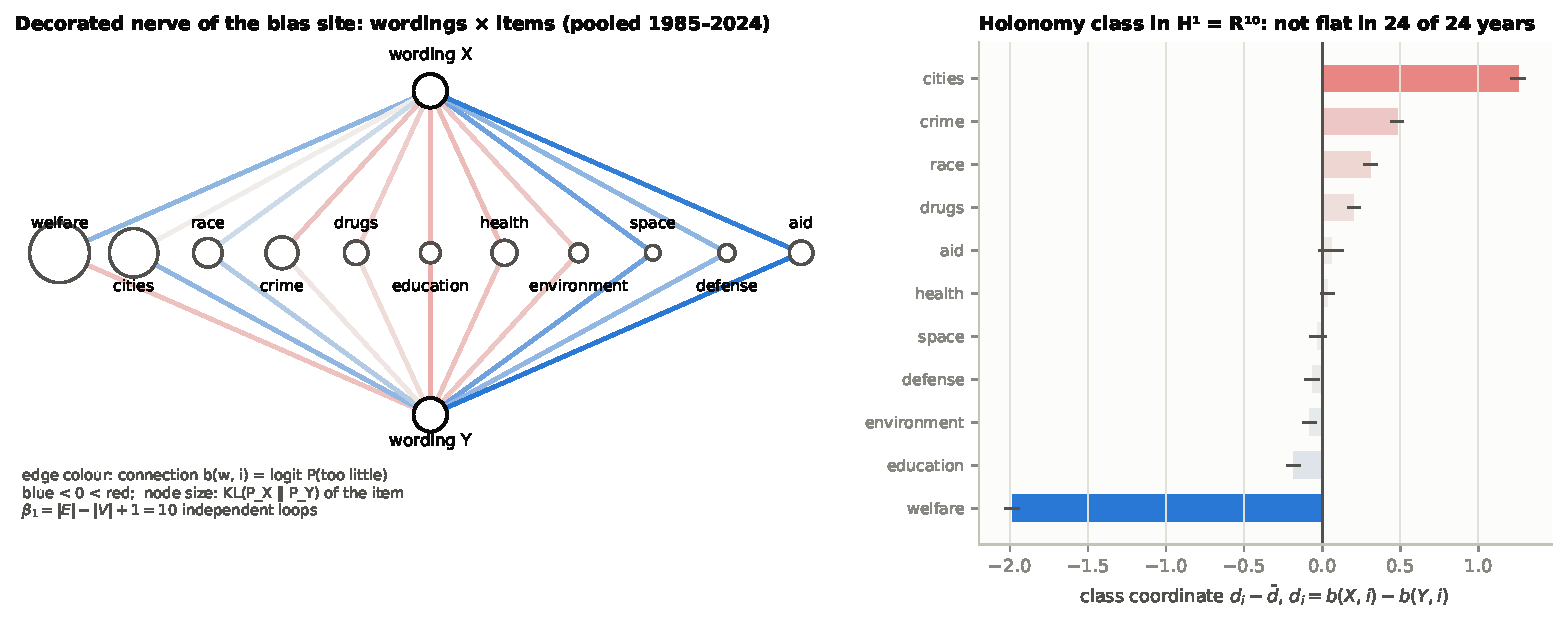
\includegraphics[width=\linewidth]{figs/fig_nerve.pdf}
\caption{Left: the bias site of the wordings as a graph $K_{2,11}$, wordings joined to items; each edge carries the connection
$b(w,i)=\operatorname{logit}P(\text{too little}\mid w,i)$, the mean over the years, and each item is decorated with the Bregman divergence
$D_{KL}(P_X\Vert P_Y)$ of its two wordings. Right: the holonomy class, the wording effects $d_i=b(X,i)-b(Y,i)$ modulo a common constant,
pooled over the years with $95\%$ intervals.}\label{fig:nerve}
\end{figure}

In ThreeLayers' bias site \cite[\S36]{ThreeLayers}, a connection on a graph is flat when it is a coboundary, a sum of a lean of each
source and an effect of each topic, and its holonomy around a cycle is the loop sum $\Phi$. Here the sources are the two wordings and the
topics the eleven items: the graph $K_{2,11}$ has $\beta_1=22-13+1=10$ independent cycles, the loops through two items $i,j$, with
$\Phi(i,j)=d_i-d_j$. The connection is flat exactly when the wording shifts the log-odds of ``too little'' by the same amount for every item,
and its class lives in $H^1(K_{2,11};\mathbb R)\cong\mathbb R^{10}$ \cite[Thm.~13.3]{ThreeLayers}. In every one of the $24$ years flatness is
rejected (Wald test with a bootstrap covariance, $\chi^2_{10}\ge333$; Bonferroni over the years). The class is dominated by two items with
opposite signs (\cref{fig:nerve}): the log-odds of ``too little'' are $1.96$ lower for ``welfare'' than for ``assistance to the poor'', and $1.29$ higher for ``solving the
problems of the big cities'' than for ``assistance to big cities''; crime ($0.51$) and
race ($0.34$) follow, and space, defense, environment and health are within $0.07$ of zero. Raw $d_i$ are quoted; only their differences, the loop sums, are invariant, and \cref{fig:nerve} plots $d_i-\bar d$. The yearly
values are pooled by inverse variance.

\subsection{Layer 2: dependence and the entropy brane}

Within one wording the two items have a joint law, and its distance from the maximum-entropy coupling with the same margins, the point
where the entropy brane meets the constraint brane \cite[Thm.~3.1]{Bridges}, is the mutual information $I=D_{KL}(T\Vert f\otimes g)$, the
Layer~2 invariant $\delta_tH$. Over the $2640$ tables its median is $0.024$ bits (largest $0.23$), and independence is rejected at a
Bonferroni level in $1140$ (\cref{sec:geometry} shows the brane picture).

\subsection{The three invariants dissociate}

On the same $1320$ system-years no contextuality is detected (Layer~3). The loop through the two items is non-flat in $493$
(Layer~1: $\lvert z\rvert>4.12$, Bonferroni over the system-years, with the variance of $d_i-d_j$ from the bootstrap including the
covariance of answers given by the same respondents), the items are dependent in at least one wording in $733$ (Layer~2: $G$-test at
$0.05/2640$), and both hold in $340$, of which $261$ are not even contextual at the point estimate. Across system-years the naive
contextual fraction tracks the size of the loop (Spearman $0.85$) but hardly the dependence ($0.24$ with the mutual information under
$X$), and the loop and the dependence are almost unrelated ($0.14$).

Two observations follow, and both are consistent with the stratification rather than tests of it. First, the three invariants are
nonzero or zero independently: Layer~3 is not detected where Layers~1 and~2 are nonzero, and neither of these two determines the other.
Part of this is structural, since the loop sums are functions of the margins and canonical Contextuality-by-Default absorbs every
marginal shift as direct influence; the empirical content is that what remains after the margins, the joint laws within the wordings,
does not produce contextuality, while it does carry dependence. Second, the naive contextuality of the wording experiments tracks, to a
first approximation, the Layer~1 holonomy of the wording connection, which a test with identical connections misreads as
contextuality and which Contextuality-by-Default places outside Layer~3.

\subsection{Composition and paths in the panels}

\begin{figure}[!htbp]
\centering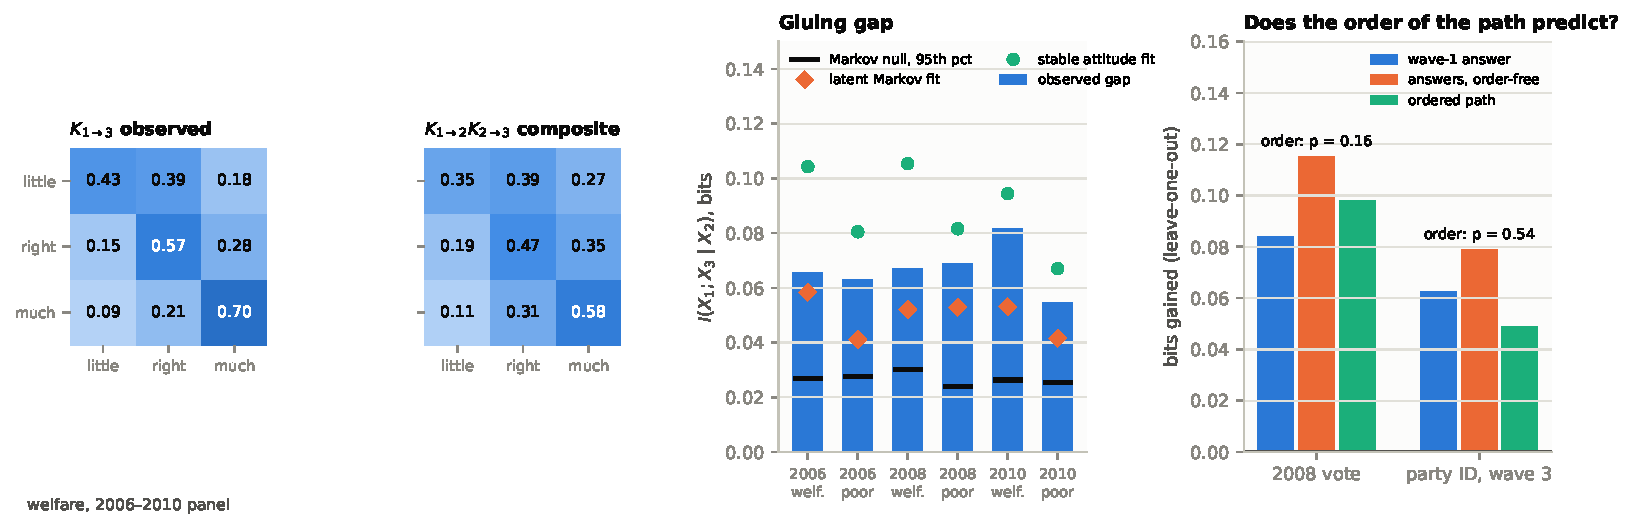
\includegraphics[width=\linewidth]{figs/fig_panels.pdf}
\caption{Left: the wave-1 to wave-3 kernel of the welfare answer and the composite of the two wave-to-wave kernels (2006--2010 panel).
Middle: the gluing gap of the answers in each series, against the $95$th percentile of the Markov null and the gaps implied by the fitted
stable-attitude and latent Markov models (\cref{tab:panelmodels}). Right: bits per respondent gained over the panel-and-wording baseline in
the association with the 2008 vote and wave-3 party identification, of the wave-1 answer, by the three answers without their order, and by the
ordered path (leave-one-out); $p$: permutation test of the order.}\label{fig:panels}
\end{figure}

The wave-1 to wave-3 kernel is not the composite of the wave-to-wave kernels: their rows differ by $0.04$ to $0.19$ in total variation,
the composite being more diffuse, as happens when the answers carry memory beyond the last wave (\cref{fig:panels}). This is the gluing
failure of \cref{tab:panels} seen in one transition, and, as shown there, a latent Markov chain answered with error reproduces it.

Does the path matter for outcomes? The vote is recalled at or after waves that belong to the path, and party identification is measured
at wave 3, so these are associations, not predictions. We compare three summaries of the answers in their association with the 2008 vote (Obama or McCain) and of wave-3 party identification
(Democrat, Independent, Republican, leaners with their party): the wave-1 answer, the multiset of the three answers (which answers were
given, regardless of order), and the ordered path, by permutation tests that permute outcomes within the cells of the smaller summary
(for the multiset against the wave-1 answer, which are not nested, the statistic is a difference of fits, not a likelihood ratio). Pooled over the six series with exact permutation tests stratified by series, the
multiset adds to the wave-1 answer ($p<0.001$ for both outcomes), but the order adds nothing to the multiset ($p=0.16$ for the vote,
$0.54$ for party), and out of sample the ordered path fits worse than the multiset ($0.098$ against $0.115$ bits gained for the vote,
$0.049$ against $0.079$ for party). Two of the twelve series-level tests of order fall below $0.05$, as expected by chance. Repeated
measurement helps because it averages unreliability; the order of the answers carries no further information about these outcomes. This
answers the question of path dependence for the survey: $K_{1\to3}\ne K_{1\to2}K_{2\to3}$ for the answers, but the difference does not
reach the outcomes.

%=====================================================================
\section{Clinical data}\label{sec:clinical}
%=====================================================================

\paragraph{Pre-registration.} The analyses of this section after NHANES, and those of \cref{sec:panels6}, follow written plans dated
before any data values were examined: a plan for MIMIC-IV (2026-10-09) and amendments for the open clinical data and for the C19PRC panels
(2026-10-10). Each plan fixes the states, thresholds, contexts, outcomes and decision rules. Each analysis program was first run on
synthetic data in the layout of its dataset, with planted answers, and recovered them all. Results were frozen with SHA-256 hashes before any
replication sample was opened. Every departure from the plans is listed in \cref{sec:deviations}. The analyses of the earlier sections
were not pre-registered.

\paragraph{The five analyses.} The same five analyses run on every clinical dataset.
\begin{enumerate}[label=\Alph*.,leftmargin=*,nosep]
\item \emph{Geometry}: regimes between contexts and the toric type of the coupling polygon.
\item \emph{Composition}: the gluing gap of three time points against a Markov null, and the stable, drifting and latent Markov models of
  \cref{tab:panelmodels}.
\item \emph{Path and outcome}: whether the multiset of three states adds to the first, and whether their order adds to the multiset.
\item \emph{Contextuality across sites or units within severity strata}: canonical CbD with the boundary null, combined by Fisher's method.
\item \emph{Selection}: the contextual fraction of three pairwise tables $(X,Y)$, $(X,Z)$, $(Y,Z)$, where $Z$ is measured only in some
  patients. It is computed available-case and compared with a sampling null. A fraction above the null means the tables are incompatible
  beyond sampling: measurement of $Z$ is not at random with respect to $(X,Y)$.
\end{enumerate}
The plans also asked for the fraction after inverse-probability weighting on the $(X,Y)$ cells, and decided ``selection explains the
incompatibility'' when it fell below the null. That rule is uninformative, which we noticed only after the results were frozen. Cell
weighting makes the measured patients reproduce the full $(X,Y)$ table, and the weighted measured sample is then a joint law of
$(X,Y,Z)$ with all three tables as margins, so the fraction after weighting is $0$ by construction. We report it, but only the
available-case test is evidence. Weights not built on the $(X,Y)$ cells (a logistic model of measurement, or the survey's own weights) can
leave a residual. Their fraction is a weak check that those weights capture the selection.
In the programme's terms, the question is whether the three tables are margins of one law: whether a point exists in the fibre of the
measurement map over them. The deeper reading, selection as a kernel from the population to what is observed, is not used here, because
the selection kernel is unknown. Fitting it is exactly the step that cell weighting does trivially.

\emph{NHANES.} From 2009--2010 to 2011--2012, diabetes among adults went from $10.2\%$ to $11.1\%$ and the BMI classes barely moved. The
change is a bend with stress $0.08$; among adults $55+$ it is a bend with stress $0.90$, close to but below the threshold of
\cref{prop:stress}, which therefore certifies the bend. The probability of diabetes given obesity is $18\%$ overall and $31\%$ at $55+$ in
both cycles, and the system is not contextual in either test. Two cycles of a stable population are a negative control: the monitor reports
no tear where none is expected.

\emph{Medical questions.} On USMLE the update moved GPT-4 from $88.2\%$ to $84.7\%$ and GPT-3.5 from $63.5\%$ to $65.0\%$ (intact prompts);
the change is a bend apart from the near-empty wall of \cref{rem:empty}. The larger finding is \cref{tab:usmle}: damaged clinical
information changes which questions a model gets right far more than it changes how many.

\subsection{Intensive care: the PhysioNet 2012 Challenge}

The PhysioNet/Computing in Cardiology Challenge 2012 \cite{Silva2012,Goldberger2000} gives the first $48$ hours of $4{,}000$ adult ICU stays
in each of two independent sets, with in-hospital death.
\begin{itemize}[leftmargin=*,nosep]
\item States: the hemodynamic state in three windows (hours $0$--$6$, $21$--$27$, $42$--$48$) from the mean arterial pressure, banded
  below $65$, $65$--$75$ and above $75$ mmHg; there is no vasopressor variable, so shock is defined by pressure alone.
\item Covariates: the first creatinine and lactate of the first day, banded, and mechanical ventilation.
\item Contexts: the ICU type (coronary, cardiac surgery, medical, surgical).
\item Design: set~A is the analysis sample and set~B the replication.
\end{itemize}
The negative control passes: the system (hemodynamic state, creatinine) moves from set~A to set~B by a bend with stress $0.83$, below one.

\begin{table}[ht]
\centering\footnotesize
\caption{PhysioNet 2012, analysis and replication sets. Gaps in bits; $p$-values of the latent-class models from the $\chi^2$ reference; the
selection row gives the available-case contextual fraction and the $95$th percentile of the sampling null.}\label{tab:icu}
\begin{tabular}{lccc}
\toprule
decision & set A & set B & replicated\\
\midrule
answers not glued (gap vs Markov null) & yes ($0.0165$ vs $0.0039$) & yes ($0.0175$ vs $0.0042$) & yes\\
latent Markov model not rejected (3 time points) & yes ($p=0.089$) & no ($p=0.008$) & no\\
death: multiset adds to the first state & yes ($p=0.023$) & yes ($p=0.016$) & yes\\
death: order adds to the multiset & no ($p=0.97$) & no ($p=0.21$) & yes\\
medical vs surgical ICU contextual, strata $H_1$ & no ($p=1.0$) & no ($p=1.0$) & yes\\
the same, strata SOFA & no & no & yes\\
lactate tables incompatible (available case) & yes ($0.0453$; $0.0365$) & yes ($0.0391$; $0.0364$) & yes\\
\bottomrule
\end{tabular}
\end{table}

Six of the seven decisions replicate (\cref{tab:icu}). Lactate is measured in about half of the stays. The available-case tables of
(first-window state, creatinine, lactate) are incompatible beyond sampling in both sets, so lactate is not measured at random with
respect to the first-window state and creatinine. (Weighting on their cells gives $0$, by construction.) ICU types differ by decided tears:
coronary against cardiac surgery and cardiac surgery against medical in both sets. Within severity strata, no difference between medical
and surgical ICUs is detected as contextual. The hemodynamic states do not compose. Three time points do not decide whether a latent
Markov chain explains this: it is not rejected in set~A ($p=0.089$) and is rejected in set~B ($p=0.008$). The order of the three states
adds nothing detectable to the association with death.

\paragraph{Interchange recheck of the pressure bands.} The gaps in \cref{tab:icu} were computed on banded pressures, which the panels
showed can inflate them (\cref{sec:interchange}). We reran the interchange test with the window medians in $5$-mmHg bins as the raw
states. The bin edges include $65$ and $75$, so banding is an exact merge of $17$ bins into $3$; the bins are themselves a merge of a
continuous value. The plan is \texttt{PREANALYSIS\_TOWER\_ICU.md}, Part 3. On planted chains with $17$ states the test held its size
($0/20$) and had full power ($20/20$), while the monitor's banded null rejected all $20$ first-order chains.
\begin{itemize}[leftmargin=*,nosep]
\item The bands are not sufficient ($p<10^{-18}$ in both sets).
\item The corrected null is twice the monitor's: $0.0078$ against $0.0039$ in set~A, $0.0068$ against $0.0039$ in set~B.
\item The interchange defect carries $38\%$ and $24\%$ of the banded failure.
\item The observed gaps, $0.0165$ and $0.0175$, still exceed the corrected null ($p=0.0025$ in both sets).
\end{itemize}
So the ICU conclusion stands, replicated, with a correctly sized null.

\subsection{A three-level tower on PhysioNet 2012, and its Fano tubes}\label{sec:towericu}

This is the first run of the tower of \cite{Tower} on real data, planned in \texttt{PREANALYSIS\_TOWER\_ICU.md} before any model was
fitted.
\begin{itemize}[leftmargin=*,nosep]
\item \emph{Level two.} Five logistic models of in-hospital death are fitted on one sample: base rate (M0); first-window pressure (M1);
  pressure and creatinine (M2); those with ventilation and ICU type (M3); SOFA band (M4).
\item \emph{Level three.} Each model is transported with a reliability $\alpha\in\{0,\frac14,\frac12,\frac34,\frac9{10},1\}$, discounted
  towards the fit sample's base rate. The tower is the posterior over the $30$ pairs (model, reliability).
\item \emph{Conditioning.} It conditions on an evidence sample one patient at a time. On the first $200$ patients it agrees with the
  programme's tower code to $2\times10^{-14}$, and coherence $\mu\Omega=\Pi$ holds throughout.
\item \emph{Test.} Its predictions are scored on a held-out test sample against flat Bayesian model averaging, which is the same
  posterior with $\alpha=1$ only.
\end{itemize}
On planted data the adapter recovered a planted reliability of $\frac12$ and then beat flat averaging, and it did not beat it when the
planted reliability was $1$.

\begin{table}[!htbp]
\centering\footnotesize
\caption{The tower on PhysioNet 2012. $\Delta$: log loss of flat model averaging minus that of the tower on the test sample, with a
paired bootstrap $95\%$ interval; level three ``earns its keep'' when the interval is above $0$. The toric surface is that of the $2\times3$
system death $\times$ first-window pressure band. The third column is exploratory.}\label{tab:towericu}
\setlength{\tabcolsep}{3pt}
\begin{tabular}{>{\raggedright}p{3.6cm}>{\raggedright}p{3.6cm}>{\raggedright}p{3.6cm}>{\raggedright\arraybackslash}p{3.6cm}}
\toprule
 & same population: fit A, evidence and test B & shift: fit surgical, evidence and test medical/coronary & shift, reliability floor = evidence base rate\\
\midrule
fit / evidence / test & $4{,}000$ / $2{,}000$ / $2{,}000$ & $1{,}942$ / $1{,}013$ / $1{,}013$ & same\\
level 2 posterior & M3: $1.00$ & M3: $1.00$ & M3: $1.00$\\
level 3 posterior & $\alpha=1$: $0.95$; $\alpha=\frac9{10}$: $0.05$ & mass on $\alpha<1$: $0.56$ & $\alpha=\frac12$: $0.50$; $\alpha=\frac34$: $0.42$\\
$\Delta$ (interval) & $-0.00001$ ($-0.00006$, $0.00005$) & $0.00016$ ($-0.00087$, $0.00123$) & $0.0091$ ($0.0025$, $0.0161$)\\
level three earns its keep & no (as predicted) & no (predicted yes) & yes\\
predicted / observed death rate & $0.141$ / $0.141$ & $0.132$ / $0.184$ & $0.148$ / $0.184$\\
toric surface: tower's posterior & $\mathbb F_1$ with $1.00$ & $\mathbb{CP}^2$ with $1.00$ & $\mathbb F_1$ $0.53$, $\mathbb{CP}^2$ $0.47$\\
toric surface of the observed system & $\mathbb F_1$, not decided on its bands & $\mathbb F_1$, not decided on its bands & same\\
tears of the level-one tube & none & none & six wall crossings\\
level-one obstruction of the observed rate & none & $d_1=0.107$, equal to the certificate margin & --\\
\bottomrule
\end{tabular}
\end{table}

\paragraph{Results (\cref{tab:towericu}).}
\begin{itemize}[leftmargin=*,nosep]
\item \emph{Same population.} Between two random halves of one population the tower behaves as predicted. Level three puts $95\%$ on
  full reliability and adds nothing to flat averaging, and the predictions are calibrated.
\item \emph{Shift.} Models fitted on surgical units and carried to medical and coronary units are the case where level three should
  earn its keep. As predicted, it moved more than half its mass below full reliability. Against the prediction, it did not improve the
  forecasts, and they stayed badly calibrated ($0.132$ against $0.184$).
\item \emph{Why the shift arm failed.} The tower's own lifting criterion explains it \cite[Thm.~10.5, Thm.~10.8]{Tower}. Every
  hypothesis predicts a death rate between $0.096$ and $0.132$, so the observed $0.184$ lies outside the admissible set at level one.
  The certificate measures the gap, $d_1=0.107$. Discounting towards the fit sample's base rate can only pull predictions down towards
  $0.102$, while the shift raised mortality. The reliability level as specified cannot represent this shift.
\item \emph{An exploratory repair, not pre-registered.} With the floor set to the evidence sample's base rate, level three does earn its
  keep ($\Delta=0.0091$, interval above $0$). Its posterior concentrates between $\alpha=\frac12$ and $\frac34$. Calibration improves to
  $0.148$ but is still short of $0.184$.
\end{itemize}

\paragraph{Fano tubes.} Each gradation of the tower predicts the death margin $f_1$ of the $2\times3$ system death $\times$
first-window pressure band, with the pressure margin $g$ observed. The pair $(f_1,g)$ fixes the coupling polygon, the moment polygon of
a toric Fano surface \cite[Prop.~8.1]{Bridges}. Here the relevant wall is $f_1=g_0$, the death rate against the share in shock.
\begin{itemize}[leftmargin=*,nosep]
\item On one side of the wall the polygon is a triangle ($\mathbb{CP}^2$); on the other it is a quadrilateral ($\mathbb F_1$, the blow-up
  of $\mathbb{CP}^2$ at a point).
\item Stacking the level-one polygon over the evidence count gives a tube (\cref{fig:fano}, left). The level-two and level-three
  gradations give one polygon per hypothesis, weighted by its posterior (right). The tower therefore carries a posterior over toric
  surfaces.
\item In the same-population arm the tube stays $\mathbb F_1$, and the tower is certain of it. Yet the realized system's chamber is
  \emph{not} decided on its bands. The tower decides the type of the expected system, not of the sampled one.
\item In the pre-registered shift arm the tube never leaves $\mathbb{CP}^2$, while the observed system is $\mathbb F_1$. The tower is
  certain of the wrong surface, which is the toric face of its level-one obstruction.
\item With the repaired floor the tube runs along the wall and crosses it six times as evidence accrues. Its final posterior is split
  between the two surfaces, $0.53$ and $0.47$. That is the honest state, since the observed chamber is undecided on the bands as well.
\end{itemize}
So the toric layer is no longer only descriptive here. It turns a calibration failure into a discrete, certifiable event: the predicted
and the observed system lie in different chambers.

\begin{figure}[!htbp]
\centering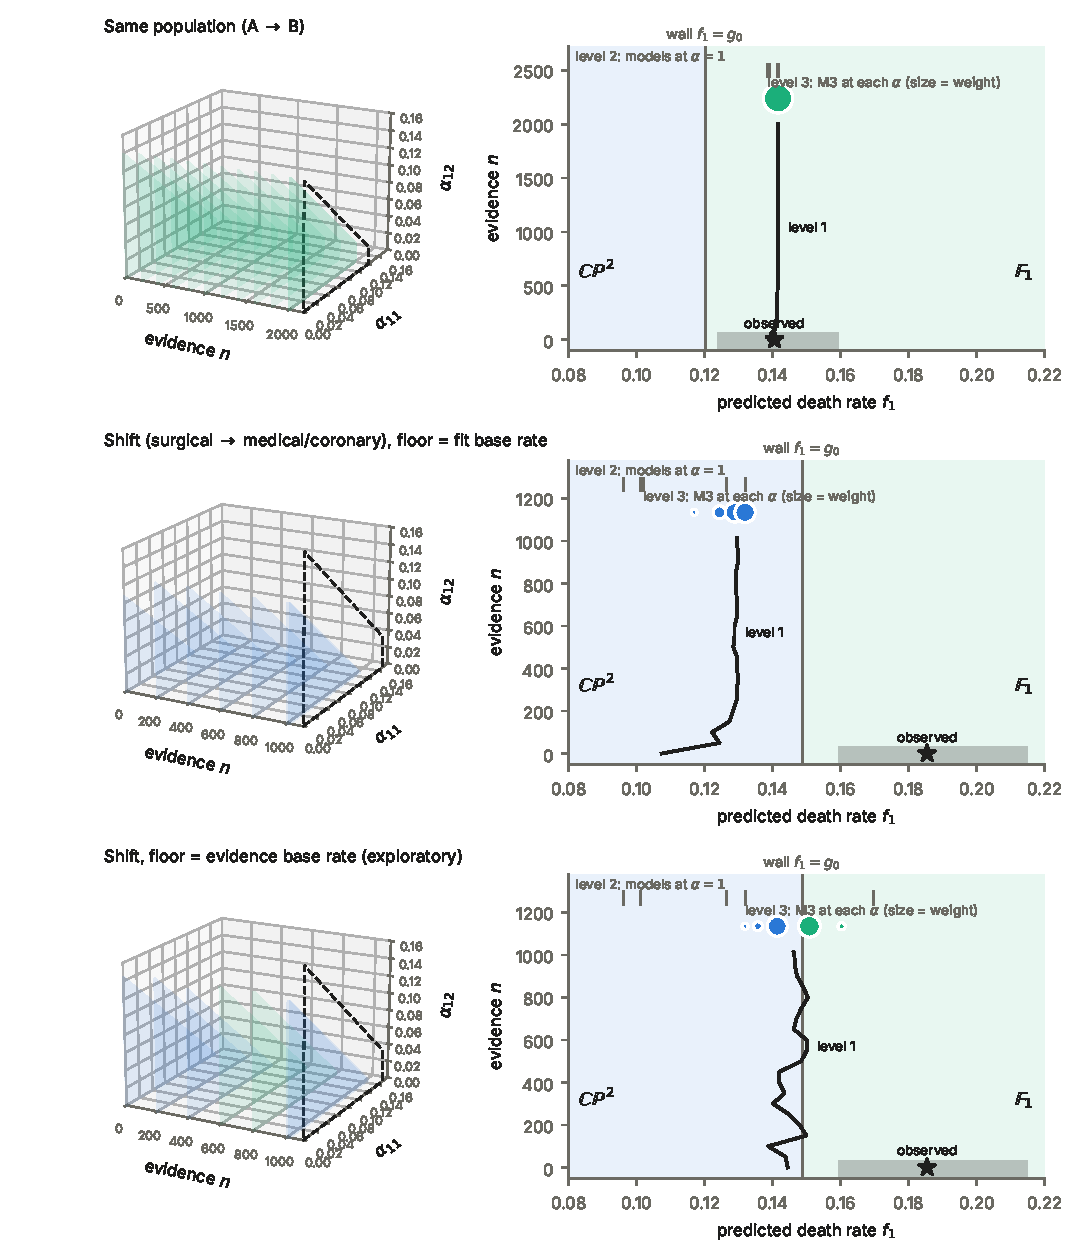
\includegraphics[width=\linewidth]{figs/fig_fano_tubes.pdf}
\caption{Fano tubes of the PhysioNet tower: same population (top), shift (middle), shift with the exploratory evidence floor (bottom).
Left: the coupling polygon of death $\times$ first-window pressure band in the coordinates $(\alpha_{11},\alpha_{12})$ at the tower's
level-one prediction, stacked over the evidence count. Colours give the toric surface: blue $\mathbb{CP}^2$ (triangle), green $\mathbb F_1$
(quadrilateral). The dashed outline is the polygon at the observed death rate. Right: the same on the axis of the predicted death rate.
The level-one path is plotted over the evidence. Level-three hypotheses (M3 at each reliability) are discs sized by posterior weight;
level-two models at full reliability are ticks. The star is the observed rate with its band. The wall $f_1=g_0$ separates the two
surfaces.}\label{fig:fano}
\end{figure}

\subsection{Diabetes: 130 US hospitals, 1999--2008}

The UCI Diabetes 130-US Hospitals data \cite{Strack2014,UCIDiabetes} record $101{,}766$ encounters of $71{,}518$ patients.
\begin{itemize}[leftmargin=*,nosep]
\item HbA1c was measured in $16.7\%$ of encounters, and the published analysis of these data is about that selective measurement
  \cite{Strack2014}.
\item With age band and readmission as the other two tables, the available-case contextual fraction is $0.0937$ against a null $95$th
  percentile of $0.0135$: HbA1c is not measured at random with respect to age and readmission. This is the clearest instance in real
  data of the selection mechanism of \cite[\S11]{Bands}. Cell weighting gives $0$ by construction. A logistic model of measurement that
  also uses admission source and type leaves $0.0081$, below the null.
\item The data are encounters that met the dataset's inclusion criteria (diabetic inpatient stays of one to fourteen days with
  laboratory tests and medications), not all admissions of these patients.
\item For the $6{,}339$ patients with at least three such encounters, the insulin regimen (none, steady, changed) does not compose across
  them: gap $0.073$ bits against a null of $0.0025$. Both twenty-parameter latent models are rejected at $5\%$ ($p=0.042$ and $0.043$),
  but not at $1\%$: weak evidence of memory in treatment beyond a latent Markov chain.
\item Encounters are ordered by encounter number, assumed chronological. Neither the later regimens (multiset, $p=0.72$) nor their order
  adds out of sample to the association with readmission at the third encounter. The order test is nominally significant ($p=0.035$),
  but the ordered path has $-0.0016$ bits of out-of-sample information relative to the base rate (the first state alone gives $0.0002$), so by the rule fixed in advance it is not
  evidence of path dependence.
\item Emergency-room and referral admissions differ by a decided tear (insulin use against readmission) and by decided toric surfaces
  ($\mathrm{Bl}_2\mathbb{CP}^2$ against $\mathbb{CP}^1\times\mathbb{CP}^1$), but within age bands no contextuality is detected ($p=1.0$).
\end{itemize}

\subsection{Heart disease: four sites}

The UCI Heart Disease data \cite{Detrano1989,UCIHeart} come from Cleveland, Budapest, Zurich and Basel, and Long Beach ($920$ patients),
and serve as an illustration.
\begin{itemize}[leftmargin=*,nosep]
\item Chest-pain type and exercise angina, within diagnosis strata: no contextuality is detected between any pair of sites (smallest
  $p=0.11$, Cleveland against Switzerland, where only $8$ patients have no disease).
\item The sites differ above all in what they measured. Fluoroscopy (\texttt{ca}) is missing for $99\%$ of the Hungarian and Long Beach
  patients and $96\%$ of the Swiss. Thallium scans are missing for $90.5\%$ in Hungary, $83\%$ in Long Beach and $42\%$ in Switzerland.
\item The available-case selection fraction is $0.0597$. It is descriptive only: no sampling null was computed for these data.
\end{itemize}

\subsection{MIMIC-IV}

The plan of \cite[\S11]{Bands} for MIMIC-IV \cite{MIMICIV}, made concrete as analyses A--E, is ready to run where the credentialed data are
held. It is tested end to end on synthetic data in the MIMIC-IV layout, which it reads directly, and writes only aggregate results with
small cells suppressed. It has not yet been run. Its analysis~E still reports the cell-weighted fraction, which is uninformative, but it now
adds the restricted selection models of \cref{sec:restricted}, each with its own null. Their external covariates are admission type and age
band. The plan was amended before any run.

\subsection{Deviations from the plans}\label{sec:deviations}

The second, third and fourth were fixed in the programs before they ran on the real files. The first was found when the UK program
first ran. The last two were found after the results were frozen, in an independent review.
\begin{itemize}[leftmargin=*,nosep]
\item \emph{UK wave membership.} The plan used the archive's \texttt{WAVE\_1} and \texttt{WAVE\_2} indicators, but they are empty in the
  released file. A respondent is counted at waves~1 and~2 if their scores for that wave are present.
\item \emph{Irish recontact at wave~5.} Wave~5 has no recontact flag. A wave-5 respondent counts as recontacted if they took part at
  wave~1.
\item \emph{Order of the C19PRC strands.} The Irish plan was written first, as the primary analysis. The UK archive arrived before any
  Irish value had been examined (only its metadata). The UK amendment then made the UK strand primary and the Irish strand the
  replication.
\item \emph{Heart Disease.} The number of vessels (\texttt{ca}) is clipped to $0$, $1$, $2+$, and age is banded $<50$, $50$--$59$,
  $60+$; neither is specified in the plan.
\item \emph{Four-wave bootstrap.} The frozen four-wave test fitted the observed table with $20$ EM starts and each bootstrap table with
  $4$. Fewer starts fit worse, inflating bootstrap $G^2$ and biasing the $p$-value upward. We reran with $8$ starts for both
  (\cref{sec:panels6}); both values are reported.
\item \emph{Selection after weighting} is $0$ by construction, as explained above; the planted synthetic test could not have shown this,
  because it planted selection on the weighting cells.
\end{itemize}

%=====================================================================
\section{Six waves: composition on latent states}\label{sec:panels6}
%=====================================================================

Three time points cannot decide whether answers that do not compose are a latent Markov chain seen with error: the latent Markov model
is not rejected in some three-wave samples and is rejected in others (\cref{tab:panelmodels,tab:icu}). With four waves it has $54$
nominal degrees of freedom. The COVID-19 Psychological Research Consortium panels \cite{McBride2021} supply them. The UK strand (primary) has six
waves, March 2020 to Autumn 2021, and $2{,}025$ respondents at wave~1. The Irish strand \cite{SpikolIE} (replication) has five waves and
$1{,}041$ respondents at wave~1.
\begin{itemize}[leftmargin=*,nosep]
\item State: depression from the PHQ-9 \cite{Kroenke2001}, banded $0$--$4$, $5$--$9$ and $10$ or more.
\item Model: the latent Markov model over four waves, with three classes, time-varying transitions and one response law. It is tested by
  $G^2$ with a parametric-bootstrap $p$-value ($200$ draws; $100$ for the free response law), because the $81$-cell table is sparse and
  some parameters sit on the boundary.
\item Check on planted data ($n=800$): it does not reject a planted first-order chain ($p=0.44$) and rejects planted second-order memory
  ($p=0.033$).
\item Power at the actual sample sizes, against the same planted memory ($8$ replicates, $40$ bootstrap draws each): $3$ of $8$
  rejections at $n=771$ and $0$ of $8$ at $n=327$.
\end{itemize}

\begin{table}[ht]
\centering\footnotesize
\caption{C19PRC panels, depression (PHQ-9 bands). B1: waves 1--3, latent-class $p$-values from the $\chi^2$ reference; B2: waves 1--4,
parametric-bootstrap $p$-values; B3: all waves, conditional gaps $I(D_{t-2};D_t\mid D_{t-1})$ in bits; E: available-case contextual
fraction against the $95$th percentile of the sampling null.}\label{tab:c19}
\setlength{\tabcolsep}{3pt}\begin{tabular}{p{4.2cm}p{4.4cm}p{3.9cm}c}
\toprule
decision & UK (primary) & Ireland (replication) & replicated\\
\midrule
B1 answers not glued & yes ($n=950$; $0.057$ vs $0.016$) & yes ($n=418$; $0.062$ vs $0.037$) & yes\\
B1 latent Markov not rejected (3 waves) & yes ($p=0.50$) & no ($p=0.042$) & no\\
\textbf{B2 latent Markov not rejected (4 waves)} & \textbf{yes} ($n=771$; $G^2=50.6$, $54$ df, $p=0.89$) & \textbf{yes} ($n=327$; $G^2=64.2$, $p=0.45$) & \textbf{yes}\\
B2, free response law per wave & not rejected ($p=0.72$) & not rejected ($p=0.32$) & yes\\
B2 power against planted memory & $3/8$ & $0/8$ & --\\
B3 gaps of the answers & $0.057$--$0.099$, all above null ($n=582$) & $0.066$--$0.148$, all above null ($n=271$) & yes\\
C order adds to the multiset (outcome) & no ($p=0.57$) & not estimable & --\\
D recontact vs fresh contextual & not detected ($p=1.0$) & not detected ($p=0.48$) & yes\\
E attrition: tables incompatible & yes ($0.0546$; $0.0473$) & no ($0.031$; $0.069$) & no\\
\bottomrule
\end{tabular}
\end{table}

In both countries the depression answers fail to compose at every step (\cref{tab:c19}). In the UK the gap is larger at later steps,
which is descriptive only, since the six-wave group is $582$ selected respondents. Yet a latent first-order Markov chain, observed through
an error law that is the same at every wave, is not rejected over four waves in either country. With the same number of EM starts ($8$)
for the observed table and for every bootstrap refit, the $p$-values are unchanged ($0.886$ and $0.448$; free response law $0.723$ and
$0.317$). This is consistent with the reading of \cref{sec:sites}: composition fails in the measurement, and the latent states may still
compose. It is not proof of it. Against a planted second-order memory of moderate strength, the test rejects in only $3$ of $8$
replicates at the UK sample size and in none at the Irish one, so longer memory of that size could have been missed, in Ireland almost
certainly.

In the UK the three states together are associated with a later report of having \emph{ever} had thoughts of self-harm ($p<0.001$), but
their order is not. The association is partly built in, since item~9 of the PHQ-9 asks about such thoughts. No contextuality is detected
between fresh and recontacted respondents ($p=1.0$ and $0.48$); their differences are direct influence, from panel conditioning,
attrition or recruitment. Given \cref{tab:cbdpower}, only large contextual effects are excluded; the Irish wave-5 deficit of $0.040$
($p=0.062$) is below what the test can detect. Attrition between waves~1 and~3 makes the UK available-case tables incompatible beyond
sampling ($0.0546$ against $0.0473$), so dropout is not at random with respect to wave-1 depression and anxiety. The survey's own wave-3
weights, which are not built on those cells, leave $0.0125$. In the smaller Irish strand no incompatibility is detected. Waves 7--9 of
the UK strand exist only as a report and are not used.

\subsection{Does banding create the failure? The interchange law on raw scores}\label{sec:interchange}

Every composition test above was run on banded states. Banding is not neutral: it is a merge, a deterministic non-injective kernel, and
the interchange law \cite[Prop.~6.1]{Algebras} says when gluing commutes with such a kernel. Write $\alpha$ and $\beta$ for the raw
$(D_1,D_2)$ and $(D_2,D_3)$ couplings of the PHQ-9 totals ($0$--$27$), and $b$ for the merge onto the three bands. Then
\begin{itemize}[leftmargin=*,nosep]
\item $L=b^{\mathsf T}(\alpha\cdot\beta)b$ is the banded image of the raw Markov composite;
\item $R=(b^{\mathsf T}\alpha b)\cdot(b^{\mathsf T}\beta b)$ is the banded Markov composite, the monitor's null;
\item for the observed banded $(D_1,D_3)$ table $O$, the identity $O-R=(O-L)+(L-R)$ is exact.
\end{itemize}
It splits the banded composition failure into the raw failure pushed through the bands, $O-L$, and the interchange defect created by
banding alone, $L-R$, which vanishes when the bands are sufficient. A raw first-order Markov chain has $O\approx L$ but $L\ne R$. So the
theorem predicts that the monitor's banded null is the wrong null whenever the bands are not sufficient. This is the first place where a
theorem of the deeper layers changes a data analysis, and it was suggested by the theory, not by the raw data. The plan
(\texttt{PREANALYSIS\_BANDING\_INTERCHANGE.md}) was written after the banded results were known but before any raw score was examined,
so the test is a post-hoc amendment. The correct reference is a parametric bootstrap from the raw Markov chain, banded afterwards.

\paragraph{Calibration first.} On planted raw chains with $28$ states and $n=950$, in $20$ replicates each:
\begin{itemize}[leftmargin=*,nosep]
\item for a genuine first-order raw chain, the monitor's banded null declares a composition failure in all $20$, while the interchange
  test does so in $1$;
\item against raw chains that return to the wave-1 score with probability $0.2$ or $0.6$, the interchange test rejects in $17$ and $20$.
\end{itemize}
So on banded data the monitor's composition test, as used in \cref{tab:panels,tab:icu,tab:c19}, is anti-conservative, and the
interchange-corrected test holds its size.

\begin{table}[!htbp]
\centering\footnotesize
\caption{The interchange test of banding (waves 1--3). Gaps in bits; nulls are $95$th percentiles of $400$ draws. The total variation
of the banded failure $O-R$ splits exactly into the raw part $O-L$ and the interchange defect $L-R$, with ``share'' the component of the
failure along the defect.}\label{tab:interchange}
\begin{tabular}{lcc}
\toprule
 & UK ($n=950$) & Ireland ($n=418$)\\
\midrule
banded gap $I(B_1;B_3\mid B_2)$ & $0.0567$ & $0.0617$\\
monitor's null (banded Markov chain) & $0.0164$ & $0.0367$\\
interchange-corrected null (raw Markov chain, banded) & $0.0231$ (median $0.0133$) & $0.0554$ (median $0.0325$)\\
$p$ against the corrected null & $0.0025$ & $0.022$\\
$\tfrac12\lVert O-R\rVert_1$, $\tfrac12\lVert O-L\rVert_1$, $\tfrac12\lVert L-R\rVert_1$ & $0.082$, $0.065$, $0.017$ & $0.082$, $0.058$, $0.030$\\
share of the failure along the interchange defect & $0.21$ & $0.34$\\
bands sufficient for $D_1$ / $D_3$ ($p$, homogeneity within bands) & $4\times10^{-6}$ / $2\times10^{-8}$ & $8\times10^{-5}$ / $9\times10^{-5}$\\
\bottomrule
\end{tabular}
\end{table}

\paragraph{Results.} The bands are not sufficient in either country (\cref{tab:interchange}). The interchange defect is a circulation, as
the theorem says, and carries a fifth of the banded failure in the UK and a third in Ireland. The correct null is larger than the
monitor's, by $41\%$ in the UK and $51\%$ in Ireland. The observed gap still exceeds it in both countries ($p=0.0025$ and $0.022$), so
banding does not explain the whole failure: the raw totals do not compose either. That is what the latent model of B2 predicts, since a
raw total is itself a noisy measurement, and an error kernel is stochastic, not a merge, so interchange cannot remove it. The two
readings agree. Banding inflates the apparent failure but does not create it, and what remains is consistent with measurement error on a
Markov latent state. In Ireland the margin is narrow. The raw-score gaps themselves ($1.24$ and $1.49$ bits) are dominated by the
sparsity of $28\times28\times28$ tables and are not interpreted.

%=====================================================================
\section{Toric geometry, the entropy brane and Floer theory on public data}\label{sec:geometry}
%=====================================================================

Bridges \cite{Bridges} realizes the coupling polytope $\Cpl(f,g)$ of two margins as the moment polytope of a compact toric manifold
$X_{f,g}$, the maximum-entropy coupling as the intersection of the entropy brane with the conormal brane of the marginal constraint
\cite[Thm.~3.1]{Bridges}, and the Floer-nontrivial couplings as the critical points of the Cho--Oh disc potential (\S8 there). Here every
one of these objects is computed for margins taken from the data.

\begin{figure}[!htbp]
\centering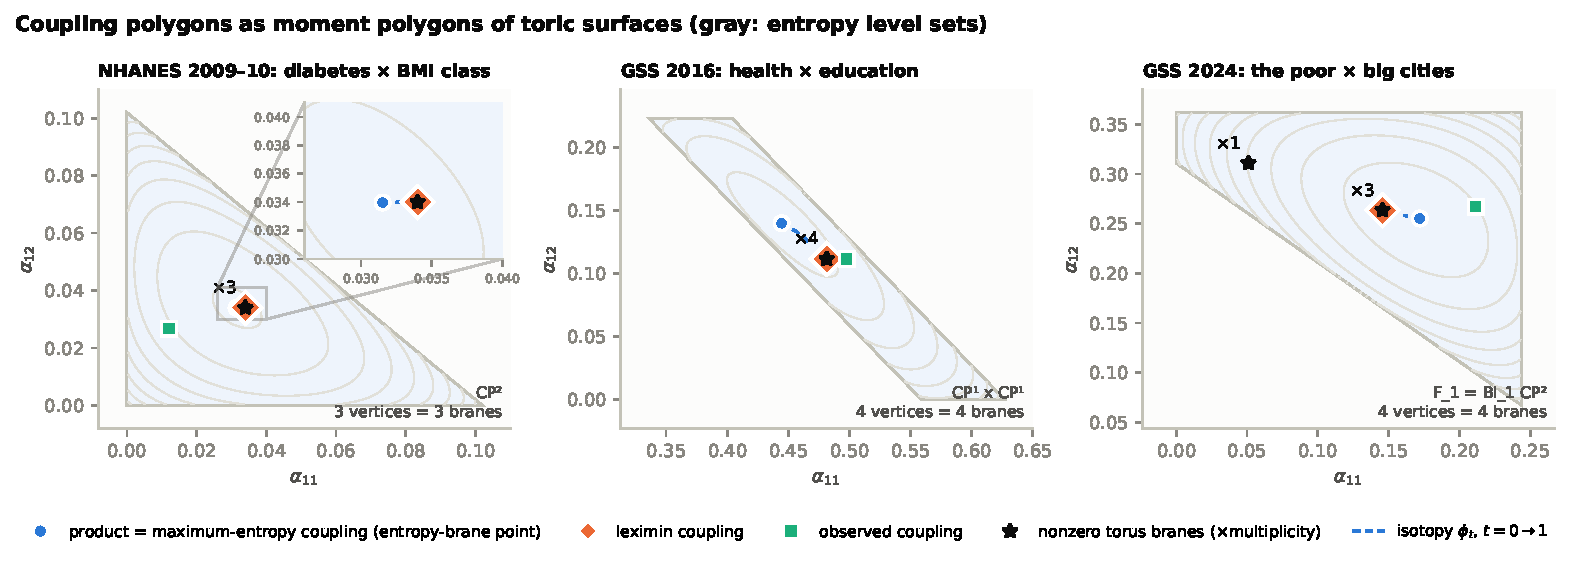
\includegraphics[width=\linewidth]{figs/fig_toric.pdf}
\caption{Coupling polygons of $2\times3$ systems with margins from the data, in the coordinates $(\alpha_{11},\alpha_{12})$. Each polygon is
the moment polygon of the toric surface named in its corner; gray curves are level sets of the entropy, whose maximum is the product
coupling. Stars are the valuations of the critical points of the disc potential (nonzero torus branes, with multiplicity), computed
exactly from Newton polygons \cite[Thm.~8.2]{Bridges}; the dashed curve is the critical point of $\phi_t=(1-t)H+t\log\prod p$ for
$t\in[0,1]$, the isotopy from the entropy brane to the standard brane \cite[Prop.~8.7]{Bridges}.}\label{fig:toric}
\end{figure}

\paragraph{Toric surfaces of real margins.} For $2\times3$ margins the toric surface is $\mathbb{CP}^2$, $\mathbb{CP}^1\times\mathbb{CP}^1$,
$\mathbb F_1$, $\mathrm{Bl}_2\mathbb{CP}^2$ or $\mathrm{Bl}_3\mathbb{CP}^2$, read off from which cells are facets \cite[Prop.~8.1]{Bridges}
(\cref{fig:toric}).
\begin{itemize}[leftmargin=*,nosep]
\item NHANES, diabetes $\times$ BMI class: $\mathbb{CP}^2$ in both cycles, decided on the bands, because only the cells of the rare row
  (diabetes) can vanish. All three nonzero branes lie over the leximin coupling, which spreads the diabetics equally over the three BMI
  classes ($\alpha_{1j}=f_1/3$); the product coupling carries none; and the observed coupling lies far from both, with diabetes concentrated
  among the obese ($\alpha_{11}=0.012$ against $0.032$ under independence in 2009--2010).
\item GSS, health (too little or not) $\times$ education, wording $X$: $\mathbb{CP}^1\times\mathbb{CP}^1$ in $15$ of $24$ years,
  $\mathrm{Bl}_2\mathbb{CP}^2$ in $6$ and $\mathbb F_1$ in $3$; the chamber, hence the surface, is decided on the bands only in 2010, 2012,
  2014, 2016 and 2021, all $\mathbb{CP}^1\times\mathbb{CP}^1$. The leximin coupling carries four branes in every year: all of them in
  the $18$ years with four vertices and four of five in the $\mathrm{Bl}_2$ years.
\item GSS, ``the poor'' (too little or not) $\times$ ``big cities'', wording $Y$: $\mathbb F_1$ in $18$ years, $\mathrm{Bl}_2$ in $4$, $\mathrm{Bl}_3$
  in $2$ (1994, 1996), never decided. The leximin coupling carries $3$ or $4$ branes, at least half of them in every year (for example
  $3$ of $4$ in $12$ years and $3$ of $6$ in one).
\end{itemize}
In all $50$ real $2\times3$ systems the product coupling carries no brane, consistent with \cite[Thm.~8.2(iii)]{Bridges}, which excludes it whenever the smallest
facet product is unique, and the leximin coupling carries at least half of the branes: on public margins, as on synthetic ones, the Floer-theoretic
distinction among couplings is robustness against breaking, not entropy. \Cref{fig:toric_years} shows the surfaces year by year; most
changes of surface are not decided, which is the toric face of the observation that most survey steps are possible tears only.

\begin{figure}[!htbp]
\centering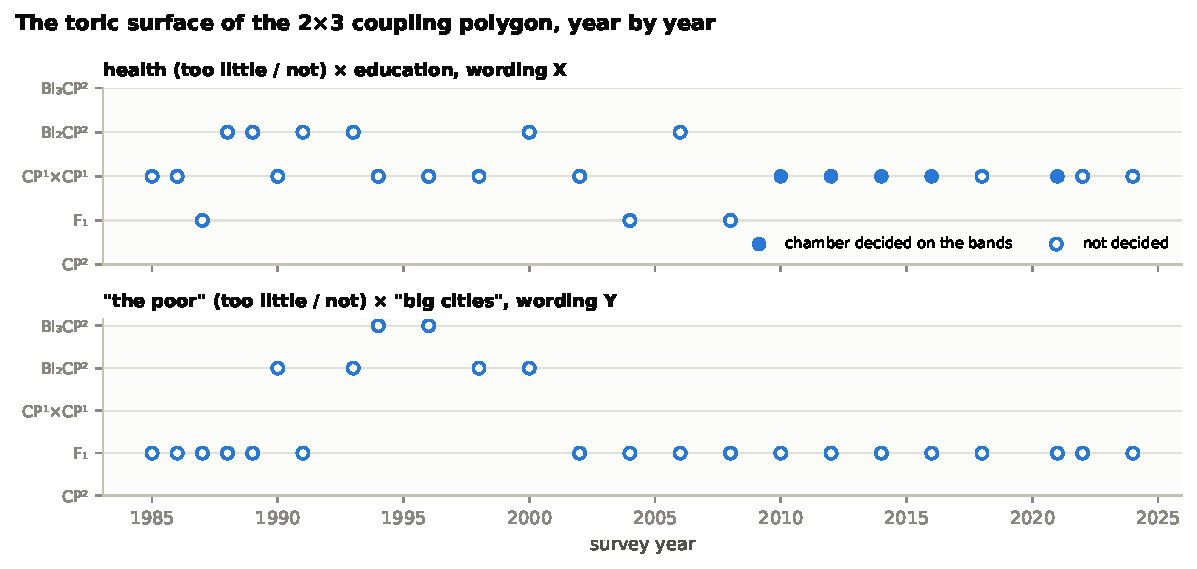
\includegraphics[width=0.82\linewidth]{figs/fig_toric_years.pdf}
\caption{The toric surface of two GSS $2\times3$ systems, 1985--2024. Filled: the chamber of the margins, which determines the surface, is
decided on the $95\%$ bands; open: it is not.}\label{fig:toric_years}
\end{figure}

\paragraph{$3\times3$ systems and tears as blow-ups.} For $3\times3$ margins $X_{P,Q}$ is a toric $4$-fold, always semi-Fano and Fano only
when the polytope has $9$ vertices, and its disc potential has no corrections \cite[Prop.~8.3, Thm.~8.4]{Bridges}. Over all $2640$ GSS
tables (pairs, years, wordings) the polytope has $9$ vertices in $54$, $12$ in $1026$, $15$ in $1070$ and $18$ in $490$. The one decided tear
of the survey, welfare $\times$ race in wording $Y$ from 2014 to 2016, takes the polytope from $15$ to $12$ vertices (\cref{fig:tearing}).
Exactly one wall changes side, $f_1=g_2+g_3$, and the facet $\alpha_{11}=0$, a tetrahedron with four vertices, disappears: the toric
$4$-fold is blown down at a torus-fixed point, the $4$-dimensional counterpart of the blow-downs of \cite[Prop.~8.1]{Bridges}. The branes of
$3\times3$ systems are not computed here.

\begin{figure}[!htbp]
\centering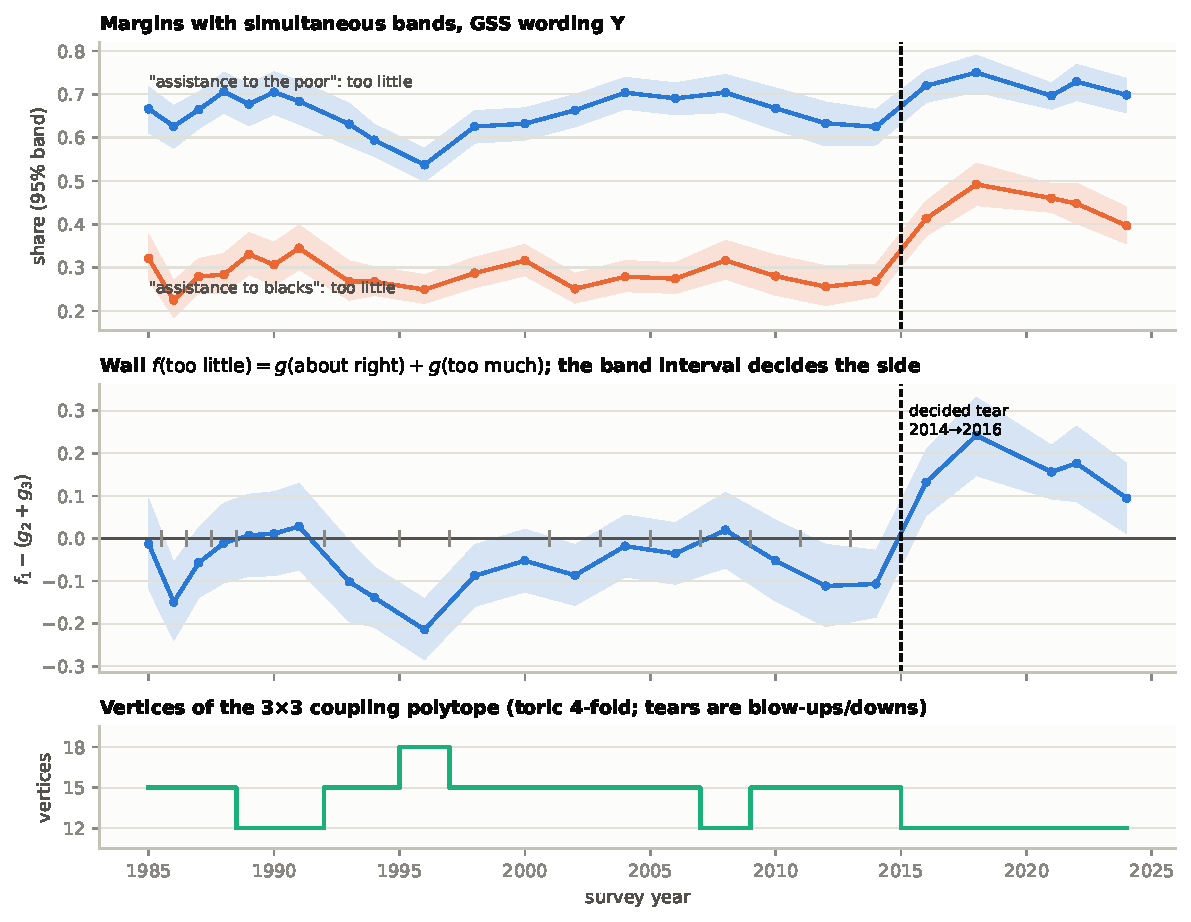
\includegraphics[width=0.72\linewidth]{figs/fig_tearing.pdf}
\caption{Forty years of one GSS system: ``assistance to the poor'' and ``assistance to blacks'', wording $Y$. Top: the ``too little''
margins with their simultaneous $95\%$ bands. Middle: the wall function whose sign changes at the tear, with the interval it takes over
the bands; the tear is decided when the intervals on both sides exclude zero; ticks mark possible tears. Bottom: the number of vertices of
the $3\times3$ coupling polytope.}\label{fig:tearing}
\end{figure}

\paragraph{The entropy brane on data.} Restricted to the fibre of a $2\times2$ system, a segment, the entropy brane is the graph of the
derivative of $H$ along the fibre, and the conormal brane is the zero section; they meet once, transversally, at the product coupling
(\cref{fig:entropybrane}, left). The distance of the observed coupling from that point is the mutual information, the Layer~2 invariant
(middle). The Hessian of $-H$ on the fibre at the intersection is the Fisher form \cite[Prop.~2.1, Thm.~3.1]{Bridges}. Its smallest eigenvalue is
positive, which is the transversality; its largest, the steepness of the intersection, diverges as a margin goes to zero, where the brane
disappears and the system breaks (for $2\times2$ systems the fibre is a segment and the two coincide). Over all $2640$ GSS $3\times3$
tables the steepness ranges from $10$ to $614$ (median $50$, right panel); it is largest where two rare answers meet, as for education
$\times$ health in 1990, where few say ``too much'' to either and the smallest product of margins is $0.0008$. These are the systems
closest to breaking, although none breaks on its bands.

\begin{figure}[!htbp]
\centering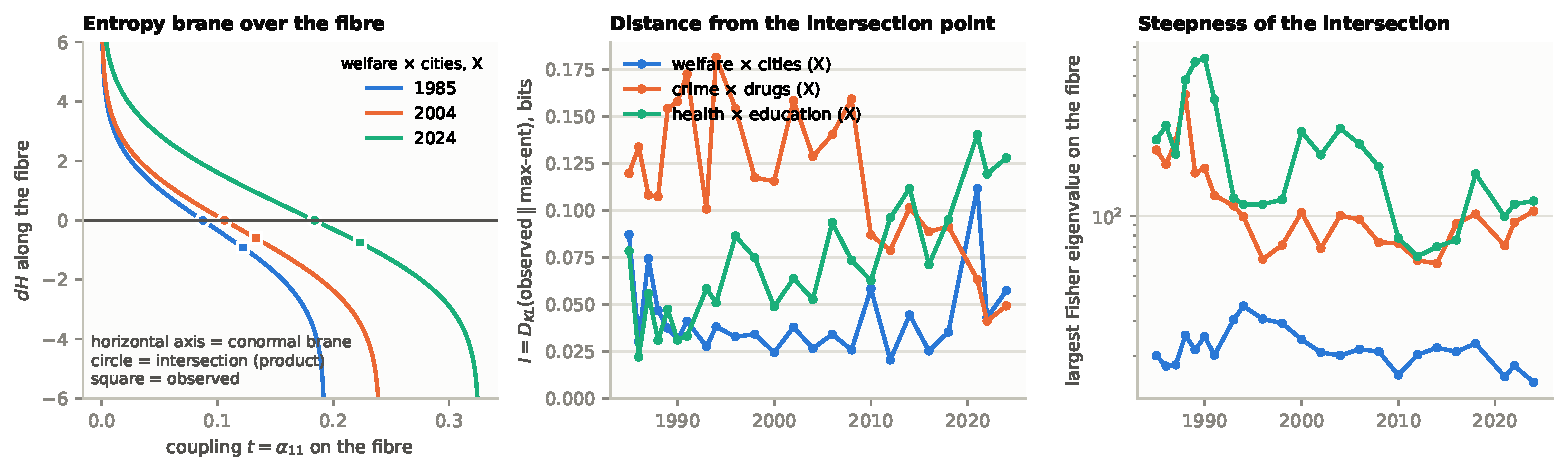
\includegraphics[width=\linewidth]{figs/fig_entropy_brane.pdf}
\caption{Left: the entropy brane over the fibre of welfare $\times$ cities (``too little'' or not, wording $X$) in three years, meeting the
conormal brane (the horizontal axis) at the product coupling; squares mark the observed couplings. Middle: mutual information, the
divergence of the observed coupling from the intersection point, for three item pairs ($3\times3$). Right: the steepness of the
intersection, the largest eigenvalue of the Fisher form on the fibre (log scale).}
\label{fig:entropybrane}
\end{figure}

\paragraph{Dual affine geometry.} The Fisher metric is the Hessian of $-H$ \cite[Prop.~2.1]{Bridges}, and its two flat structures, the
exponential (e) and mixture (m) coordinates, are Legendre dual \cite{AmariNagaoka2000}. For an m-flat family $M$ and a law $q$, the
e-projection $p^\ast$ of $q$ onto $M$ satisfies $D(p\Vert q)=D(p\Vert p^\ast)+D(p^\ast\Vert q)$ for every $p\in M$ \cite{Csiszar1975}.
\Cref{fig:fisherbregman} applies this to the two wordings of the welfare item in 2024: with $q$ the ``welfare'' law, $p$ the ``assistance to
the poor'' law and $M$ the laws with $p$'s share of ``too little'', $D(p\Vert q)=0.437$ bits splits into $0.413$ bits
carried by the shift of ``too little'' and $0.024$ bits of reallocation between ``about right'' and ``too much''. So $94\%$ of the
information in the wording effect is the shift of a single category.

\begin{figure}[!htbp]
\centering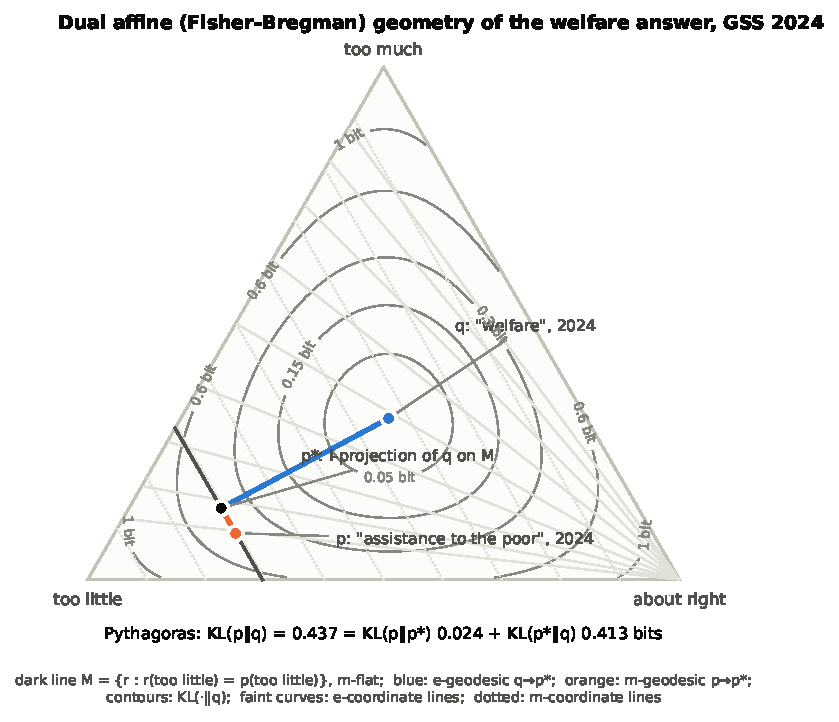
\includegraphics[width=0.62\linewidth]{figs/fig_fisher_bregman.pdf}
\caption{The simplex of answers to the welfare item, with level sets of $D(\cdot\Vert q)$, the e- and m-coordinate lines, and the
generalized Pythagorean decomposition at the e-projection $p^\ast$.}\label{fig:fisherbregman}
\end{figure}

\paragraph{Why these layers are descriptive here.} Toric surfaces, branes, the entropy brane and its steepness are computed exactly on
real margins. But nothing in these data asks a question whose answer depends on them beyond what the margins already give. A toric type
is a function of the chamber, and the chamber of the margins. The steepness grows as a margin approaches zero, which the bands already
see. The Floer data concern pairs of couplings, and no analysis here compares couplings across contexts in a way that needs them. To
activate these layers one must test a prediction: for example, that systems with steep entropy branes break sooner, or that the toric
type at one time predicts the next tear better than the distance to the nearest wall. We have not done so (\cref{sec:activation}).

%=====================================================================
\section{The structural backbone on synthetic data}\label{sec:structure}
%=====================================================================

The data of the earlier sections test bands, regimes, contextuality, holonomy, dependence, composition and selection. They cannot test
the programme's algebraic backbone: the monad of kernels and its Kleisli composition, the three-level tower, its mixed distributive law,
and the interchange of couplings with kernels. No public dataset labels its monads or contains a planted failure. We therefore built
four synthetic tests, T1--T4, under three conditions:
\begin{itemize}[leftmargin=*,nosep]
\item every expected value is a closed form, either stated in a programme paper or given by Bayes' rule in exact rational arithmetic,
  never a Monte Carlo estimate;
\item every planted failure is localized, at a known kernel, axiom, 2-cell or tower level;
\item every failure has a magnitude parameter that runs from ``the law holds'' to ``the law fails by a known amount''.
\end{itemize}
The plan, with all expected values, was written before any data were generated. One amendment was made before the first run, because
the plan had placed a defect where unitality makes it vanish identically. The data were then generated from a seed and frozen with
SHA-256 hashes, and the results frozen after a single run of each program.\footnote{The T3 program crashed once, on a vector bug in a
helper, before writing any result; it was fixed and run once to completion.} The tests call the programme's existing code for the tower,
the laws and the certificates, and check the new matrix library against the existing whiskering code (agreement to $1.1\times10^{-16}$).
Of the $41$ pre-registered expectations, $40$ hold (\cref{tab:structure}); the exception is a lesson about random-instance checks. These layers are tested on synthetic data because, as \cref{sec:activation} explains, the observational data do not supply the model spaces and channels they act on; the interchange law is the exception, and \cref{sec:interchange} applies it to real panels.

\begin{table}[!htbp]
\centering\footnotesize
\caption{Structural tests on synthetic data with closed-form ground truth (\texttt{ext/structure/}). ``Planted'' rows are failures the
papers predict; a row passes when the code reports the failure at the stated place with the stated size.}\label{tab:structure}
\setlength{\tabcolsep}{3pt}
\begin{tabular}{>{\raggedright}p{1.25cm}>{\raggedright}p{4.5cm}>{\raggedright}p{4.1cm}>{\raggedright\arraybackslash}p{4.2cm}}
\toprule
test & claim & expected & observed\\
\midrule
T3 & Kleisli composites, associativity, unit, $k^\#\mu=\mu\,\mathcal D(k^\#)$ & exact on the library & $195$ composites, $2{,}197$ triples, exact\\
T3 & invertible kernels; breaking and healing \cite[Props.~5.1, 6.4]{Bands} & the $6$ permutations; zero columns break & as predicted, every kernel\\
T3 & contraction by the Dobrushin coefficient & $\TV(K^{\mathsf T} p,K^{\mathsf T} q)\le\eta(K)\TV(p,q)$ & holds on all $15\times190$ pairs\\
T3, planted & whiskering functorial for deterministic kernels only \cite[Thm.~10.2]{Conditionals} & defect $0$ for deterministic pairs & $0$ on $48$ pairs; nonzero on all $49$ others\\
T3, planted & functoriality defect of $h_\varepsilon$ at the swap coupling & sympy closed form & $-2\varepsilon^2(1-\varepsilon)^2$, exact at $6$ values\\
T3, planted & multiplicativity defect \cite[Prop.~6.6]{Bands} & $t(\varepsilon)(1-2s)(1-2r)$, $t(\tfrac1{10})=\tfrac{369}{2500}$ & exact on $216$ cases; constant-kernel formula on $380$\\
T3, planted & integrality \cite[Thm.~6.1]{Bridges} & integral iff deterministic or constant & the $10$ predicted kernels, no others\\
T1 & sequential tower $=$ batch Bayes; coherence at every level & exact & $200$ of $200$ steps\\
T1 & \cite[Ex.~9.1]{Bands} reproduced; entropy split & table to $3$ decimals & all $32$ entries\\
T1, planted & Cromwell break at level two; reliability prevents it & weight exactly $0$ from the first $2$; never $0$ with $\alpha<1$ & as predicted; odds bound of \cite[Prop.~9.2]{Bands} holds\\
T1, planted & claims failing first at levels $1$, $2$, $3$ \cite[Thm.~10.5]{Tower} & levels $1,2,3$; $d_2=\tfrac12$, $d_3=2$ & levels $1,2,3$; $d_1=0.4=$ certificate; $d_2=\tfrac12$; $d_3=2$\\
T2 & \cite[Table~2]{Tower}: shift, averaging and base-relative laws & fail (U, M, Cm), (Cm), none & $30/30$ violations exactly where predicted\\
T2, planted & perturbed barycenter $\beta_\varepsilon$ fails (M) only & defect $\frac\varepsilon6\lVert\frac{\rho_1+\rho_2}2-\rho_3\rVert_1$ & exact at $6$ values; (U), (Co), (Cm) intact\\
T2, planted & random instances detect $\beta_\varepsilon$ for every $\varepsilon>0$ & violations iff $\varepsilon>0$ & \textbf{none at $\varepsilon=1$}\\
T4, planted & interchange \cite[Prop.~6.1]{Algebras} & holds for bijections and sufficient merges & holds; fails for the other $3$ kernels\\
T4, planted & sweep $l_t=(1-t)I+tJ/2$ & $\frac{1-(1-t)^2}4\bigl(\begin{smallmatrix}-1&1\\1&-1\end{smallmatrix}\bigr)$ & exact at $6$ values\\
\bottomrule
\end{tabular}
\end{table}

\subsection{T3: Kleisli composition and its known failures}

The library holds $15$ kernels on three points, each labelled before the run with its class:
\begin{itemize}[leftmargin=*,nosep]
\item the six permutations;
\item two constant kernels;
\item three stochastic kernels with full support;
\item two with a zero column;
\item two merges onto two points;
\item a binary family $h_\varepsilon=\bigl(\begin{smallmatrix}1-\varepsilon&\varepsilon\\\varepsilon&1-\varepsilon\end{smallmatrix}\bigr)$.
\end{itemize}
The monad laws hold exactly. Kleisli composites computed by the distribution-monad code of the tower paper agree with the matrix product
on all $195$ composable pairs, and Kleisli extensions commute with the barycenter.

The planted failures are all reproduced with their stated sizes:
\begin{itemize}[leftmargin=*,nosep]
\item \emph{Whiskering in the kernel.} Copy whiskering is functorial on all $48$ pairs of deterministic kernels and fails on all $49$
  pairs of non-deterministic ones, constant kernels included. On the binary family the defect at the swap coupling is
  $\mp2\varepsilon^2(1-\varepsilon)^2$ per entry. It vanishes only at the identity and the swap, and is largest, $\frac18$, at the constant kernel.
\item \emph{Unitality.} Copy whiskering is unital for every kernel, which is why the defect vanishes at the diagonal coupling. The product
  action is unital exactly for the eight deterministic kernels.
\item \emph{Multiplicativity.} The defect formula of \cite[Prop.~6.6]{Bands} holds exactly on all $216$ grid cases, and its
  constant-kernel form on all $380$ pairs.
\item \emph{Integrality.} Integrality holds for exactly the ten deterministic or constant kernels. So constant kernels are on the good
  side for integrality and on the bad side for whiskering, as \cite[Rem.~6.3]{Bridges} says.
\end{itemize}

\subsection{T1: the tower under a known generative model}

The generative model is the four models of a three-valued outcome given in the plan. One of them, $\rho_1=(\frac12,\frac12,0)$, has a
zero. Each model is discounted towards the uniform law with reliability $\alpha\in\{1,\frac9{10},\frac7{10}\}$, and $200$
observations are drawn from $\rho_3$ at $\alpha=\frac9{10}$. The hypotheses are the twelve pairs (model, reliability).
\begin{itemize}[leftmargin=*,nosep]
\item Level two is the posterior over models.
\item Level three is the posterior over reliabilities, each carrying its own level-two state, $\Omega=\sum_\alpha\pi(\alpha\mid
  x)\,\delta_{\Pi_\alpha}$.
\item Level one is the predictive law.
\end{itemize}

\paragraph{Coherence.} Conditioning one observation at a time with the tower code agrees exactly with the batch closed form at all $200$
steps, at every level. Coherence $\mu\Omega=\Pi$, $\mu\Pi=\rho$ holds throughout. Conditioning commutes with pooling
\cite[Prop.~9.12]{Tower}. After $200$ observations the true model has posterior $1.000$, while the reliabilities $1$ and $\frac9{10}$
are not yet separated ($0.34$ and $0.49$).

\paragraph{The Cromwell break.} The table of \cite[Ex.~9.1]{Bands} is reproduced in all $32$ entries. On the frozen data the first
observation is a $2$. In the tower without reliability, the zero model's weight is exactly $0$ from that step on and never returns: a
zero at level one becomes a break at level two. With reliability below one no weight ever reaches zero (the smallest is
$1.1\times10^{-35}$), and every odds ratio moves by at most the bound of \cite[Prop.~9.2]{Bands}.

\paragraph{Planted claims at each level.} Three claims are each detected first at the planted level, with the distance of
\cite[Thm.~10.8, Prop.~10.9]{Tower}:
\begin{enumerate}[leftmargin=*,nosep]
\item The removed model, asserted after the break, fails at level one. Its distance $0.4$ equals the margin of the optimal certificate.
\item The pre-break level-two state, here the prior, has a barycenter $(\frac38,\frac25,\frac9{40})$ inside the hull of the surviving
  models. So it passes level one and fails first at level two, with $d_2=\frac12$, twice the weight of the removed model.
\item Collapsing the reliability level into one second-order state, $\delta_\Pi$, passes levels one and two and fails first at level
  three, with $d_3=2$.
\end{enumerate}
As controls, the true tower lifts coherently, and the discounted zero model is admissible.

\subsection{T2: the mixed distributive law}

\paragraph{The paper's table.} The three laws of \cite[Table~2]{Tower} were run on $30$ random instances each, generated by the tower
paper's own scripts. Violations occur exactly where the table says, $30$ of $30$ each time:
\begin{itemize}[leftmargin=*,nosep]
\item the shift law fails (U), (M) and (Cm);
\item the averaging law fails only (Cm);
\item the base-relative law fails none.
\end{itemize}
On the paper's counterexamples each failure has size $2$ in $\ell^1$ at level one, and the shift law's failures vanish after the
barycenter, as \cite[Thm.~8.3]{Tower} states.

\paragraph{A planted law.} We replaced the barycenter of the context algebra by
$\beta_\varepsilon=(1-\varepsilon)\beta+\varepsilon\cdot(\text{uniform average over the support})$. This keeps the unit law,
naturality and coherence, so the perturbed law should fail only the multiplication axiom (M). It does. On the pre-registered
instance the level-one defect is $\frac\varepsilon6\lVert\frac{\rho_1+\rho_2}2-\rho_3\rVert_1=\varepsilon/126$ exactly, for every
$\varepsilon$.

\paragraph{The failed expectation.} At $\varepsilon=1$, the random-instance check finds no violation in $20$ instances, although the
law fails (M). The generator of the existing checks draws two-point samples, and a uniform average over supports of equal size is
associative. So that generator has no power against this failure. A random-instance check that passes is evidence only against the
failures its generator can produce (\cref{sec:better}).

\subsection{T4: interchange of couplings and kernels}

The identity $k^{\mathsf T}(\alpha\cdot\beta)m=(k^{\mathsf T}\alpha l)\cdot(l^{\mathsf T}\beta m)$ of \cite[Prop.~6.1]{Algebras} behaves as stated:
\begin{itemize}[leftmargin=*,nosep]
\item It holds exactly for bijections, and for a merge that is sufficient for the first coordinate. This was checked both with identity
  outer kernels and with stochastic ones.
\item It fails for the same merge on generic couplings ($\ell^1$ defect $0.18$), for a constant kernel ($0.18$) and for a stochastic one
  ($0.18$). Stochastic outer kernels contract the defect to $0.004$--$0.006$.
\item The defect is a circulation every time.
\item Along $l_t=(1-t)I+\frac t2J$ the defect is $\frac{1-(1-t)^2}4\bigl(\begin{smallmatrix}-1&1\\1&-1\end{smallmatrix}\bigr)$ exactly,
  $0$ only at the identity.
\end{itemize}
Vertical composition is coherent: gluing is strictly associative and unital on $216$ triples, and cost is subadditive on $100$ pairs.

\paragraph{What these tests show.} They show that the code implements the structures the papers state, and that each failure the papers
predict appears where predicted, with the predicted size. They do not prove the theorems beyond the finite cases checked; the proofs do
that. Nor do they show that any of this structure matters in data; that is the subject of the earlier sections, and of
\cref{sec:better}.

%=====================================================================
\section{Forecasting, selection, events and the tower's reliability}\label{sec:phase4}
%=====================================================================

The preceding sections left four questions open. They were pre-registered together in one plan
(\texttt{PREANALYSIS\_PHASE4.md}), checked on planted data and run once:
\begin{enumerate}[leftmargin=*,nosep]
\item Do toric type, chamber transitions or brane steepness forecast anything beyond the margins?
\item Which selection models, not built on the triangle cells, fit the data?
\item Do structural events track external states?
\item Can a richer reliability level repair the tower's failure under a shift?
\end{enumerate}
Two deviations were recorded. A planted design in the selection check was changed before the real run (below). The structural-event
analysis was run in the same command as its first planted check; that check's planted confounding was too weak, and a stronger check
was then run and passed.

\subsection{Does geometry forecast beyond the margins?}\label{sec:forecast}

Toric type, chamber and steepness are deterministic functions of the margins. So the right baseline is not a linear model in the
margins but a flexible one (B2: margins with all squares and products). The question is whether these particular functions add to a
generic nonlinear function of the same margins. Geometry (S2 = B2 plus the geometric features) is said to forecast beyond the margins
when its test log-loss gain over B2 has a bootstrap interval above $0$. The adapter detected a planted geometric signal and correctly
found none when the signal was purely marginal.

\paragraph{Clinical deterioration.} For each ICU stay and each day, the hourly mean arterial pressure band and heart-rate band form a
$3\times3$ system whose margins are the shares of hours.
\begin{itemize}[leftmargin=*,nosep]
\item \emph{Features.} Vertex counts and their change (blow-ups and blow-downs), wall flips between the two days, the tear margin, break
  counts and the steepness of day two.
\item \emph{Fit and test.} Fit on set A ($3{,}758$ stays), tested on set B ($3{,}802$ stays, $549$ deaths).
\item \emph{Death.} Geometry adds nothing: gain $0.0004$, interval $(-0.0020, 0.0027)$; over the linear baseline, $0.0005$,
  $(-0.0014, 0.0026)$.
\item \emph{Onset of shock on day two.} Nothing either: $0.0002$, $(-0.0006, 0.0009)$.
\end{itemize}
The reason is visible in the data. $98.8\%$ of day-two systems have a zero margin, typically no hours in one pressure or rate band, and
half have a coupling polytope that is a single point. Per-stay systems of a day live almost entirely in the breaking regime, where the
toric layer has nothing to describe. A finer time grid or a longer window would be needed to give these systems a nondegenerate geometry.

\paragraph{Societal transitions.} The GSS item-pair systems ($110$ systems in two wordings) were followed from one survey year to the next.
The event is a change of the point-estimate chamber. Decided tears are too rare to forecast (one in the paper). Training used steps
ending by 2004 ($1{,}320$) and testing those from 2006 on ($1{,}100$), with intervals clustered by system. Here geometry forecasts
beyond the margins: gain $0.041$, interval $(0.020, 0.062)$; over the linear baseline $0.038$, $(0.017, 0.058)$. Most of it is carried
by two quantities:
\begin{itemize}[leftmargin=*,nosep]
\item the tear margin: the chamber changes at the next survey in $71\%$ of the systems in the quartile nearest a wall, and in $33\%$ of
  the farthest;
\item a change at the previous step: $66\%$ against $42\%$.
\end{itemize}
The event is a change of the \emph{point estimate}, and a system near a wall flips by sampling noise as well as by change. So this shows
that the programme's distance to the walls predicts chamber instability, which raw margin shifts do not. It does not show that geometry
predicts substantive tears.

\subsection{Restricted selection models}\label{sec:restricted}

Weighting on the cells of the fully observed table makes the triangle compatible by construction (\cref{sec:clinical}). The
restricted models each have their own null: tables compatible and selection following the model, simulated and refitted at every draw
(\cref{tab:restricted}). Their weights depend on:
\begin{itemize}[leftmargin=*,nosep]
\item one content only;
\item covariates outside the triangle;
\item one content plus those covariates.
\end{itemize}
One fact limits every such test. Any weights that reproduce the full $(X,Y)$ table make the weighted measured sample a joint law with the
three tables as margins, so the tables are compatible. So these tests check only what each model implies about the $(X,Y)$ composition of
the measured units. Selection that biases $Z$ within $(X,Y)$ cells, on $Z$ itself or on a covariate that drives $Z$ but not $(X,Y)$, is
invisible to the triangle. The planted check had to be redesigned for this reason before the real run. Its first version planted
selection on a covariate independent of $(X,Y)$, which leaves the triangle compatible whatever the weights.

\begin{table}[!htbp]
\centering\footnotesize
\caption{Restricted selection models: weighted contextual fraction against the $95$th percentile of its own null ($200$ draws);
``fits'' when at or below. Cell weighting gives $0$ by construction and is omitted.}\label{tab:restricted}
\setlength{\tabcolsep}{3pt}
\begin{tabular}{>{\raggedright}p{5.0cm}ccccc}
\toprule
 & available case & $X$ only & $Y$ only & external & $X$ + external\\
\midrule
PhysioNet A: lactate; $X$ pressure, $Y$ creatinine; ICU type, ventilation & $0.045$ & $0.040$ / $0.016$ & $0.026$ / $0.016$ & $0.068$ / $0.021$ & $0.062$ / $0.019$\\
PhysioNet B (replication) & $0.039$ & $0.033$ / $0.015$ & $0.031$ / $0.015$ & $0.055$ / $0.022$ & $0.049$ / $0.020$\\
Diabetes: HbA1c; $X$ age, $Y$ readmission; admission source and type & $0.094$ & $0.016$ / $0.007$ & $0.093$ / $0.008$ & $0.097$ / $0.009$ & $0.018$ / $0.008$\\
C19PRC UK attrition: $D_3$; $X$ $D_1$, $Y$ $A_1$; age, gender, education, urbanicity & $0.055$ & \textbf{$0.012$ / $0.017$} & $0.022$ / $0.017$ & \textbf{$0.020$ / $0.023$} & \textbf{$0.010$ / $0.021$}\\
\bottomrule
\end{tabular}
\end{table}

\begin{itemize}[leftmargin=*,nosep]
\item \emph{UK panel.} Dropout between waves~1 and~3 is consistent with selection on wave-1 depression alone, on demographics alone, or
  on both. It is not consistent with selection on wave-1 anxiety alone.
\item \emph{ICU lactate.} In both sets every restricted model is rejected. Lactate is ordered according to pressure and creatinine
  \emph{jointly}, and the ICU type and ventilation make the fit worse, not better.
\item \emph{Diabetes.} HbA1c testing is mostly explained by age ($0.094\to0.016$) but not entirely, and readmission and admission route
  add nothing.
\end{itemize}
The same models, with admission type and age band as the external covariates, are now part of analysis E of the MIMIC-IV kit. Its
synthetic check recovers a planted creatinine-only selection and rejects the other models ($9$ of $9$ checks).

\subsection{Structural events against external states}\label{sec:events}

A pipeline (\texttt{structural\_events.py}) turns any sequence of systems into events: blow-ups and blow-downs (the vertex count of the
coupling polytope going up or down, a change of toric type), chamber transitions, breaks appearing or healing, and steepness. It tests
their association with an external state by permutation, crude and within strata.
\begin{itemize}[leftmargin=*,nosep]
\item \emph{ICU deaths} ($7{,}560$ stays, day one to day two). No structural event is associated with death, crude or within deciles
  of the margin-based risk. Blow-ups carry $15.1\%$ mortality against $14.0\%$ ($p=0.26$, within deciles $0.46$); breaks appearing,
  $13.7\%$ against $14.5\%$ ($p=0.39$).
\item \emph{Partisanship.} Across $22$ GSS year-to-year steps, the share of item-pair systems that change chamber correlates with the
  size of the change in Republican identification at Spearman $0.35$ ($p=0.11$). The direction is suggestive, but $22$ steps cannot
  decide it.
\item \emph{Hallucination thresholds.} For the eight retraining tasks we tabulated the regime against the change in incorrect and invalid
  answers, without a test. The three decided tears are among the four tasks with the largest increase in incorrect answers: HotpotQA,
  counting happy numbers and primality. The exception is LeetCode, a bend with a $31$-point rise.
\end{itemize}
The pipeline is general. What it lacks is data with many units, a nondegenerate geometry and an external state measured at the same
grain.

\subsection{A generalized reliability level for the tower}\label{sec:gentower}

Level three now carries a family of floors. A model's prediction $\rho$ is transported as $\alpha\rho+(1-\alpha)\varphi$, with $\varphi$
on a grid from $0.05$ to $0.40$. This is the Kleisli composite of $\rho$ with a binary channel, so the reliability level is a posterior
over channels, not over a scalar. It is compared with the fixed floor of \cref{sec:towericu} and with the evidence-rate floor found there
after the fact, which was pre-registered here. Since no new ICU data are open, replication uses four new splits of PhysioNet:
\begin{itemize}[leftmargin=*,nosep]
\item the sets reversed (R1);
\item three shifts between unit types (R2--R4), in both directions of mortality.
\end{itemize}
On planted data the variants behaved as intended: under a planted prevalence shift both new variants earned their keep, and without one
none harmed.

\begin{table}[!htbp]
\centering\footnotesize
\caption{The tower's reliability level across arms: gain in test log loss over flat model averaging, with $95\%$ interval, and the
predicted death rate. Bold: the interval is above $0$.}\label{tab:gentower}
\setlength{\tabcolsep}{2.5pt}
\begin{tabular}{>{\raggedright}p{4.1cm}>{\centering}p{1.6cm}>{\centering}p{1.2cm}>{\centering}p{2.5cm}>{\centering}p{2.5cm}>{\centering\arraybackslash}p{1.4cm}}
\toprule
arm (fit $\to$ evidence and test) & death rate (fit / test) & fixed floor & evidence floor & family of floors & predicted (family)\\
\midrule
R0a same population, A $\to$ B & $0.139$ / $0.141$ & $0.0000$ & $0.0000$ & $0.0000$ & $0.141$\\
R0b shift, A surgical $\to$ B medical & $0.102$ / $0.184$ & $0.0001$ & $\mathbf{0.0090}$ $(0.002, 0.016)$ & $\mathbf{0.0125}$ $(0.005, 0.020)$ & $0.164$\\
R1 same population, B $\to$ A & $0.142$ / $0.135$ & $0.0008$ & $0.0008$ & $0.0007$ & $0.138$\\
R2 shift, B surgical $\to$ A medical & $0.106$ / $0.165$ & $0.0014$ & $\mathbf{0.0086}$ $(0.002, 0.016)$ & $\mathbf{0.0111}$ $(0.001, 0.021)$ & $0.162$\\
R3 shift, A medical $\to$ B surgical & $0.173$ / $0.105$ & $-0.0004$ & $0.0040$ $(-0.001, 0.009)$ & $\mathbf{0.0083}$ $(0.003, 0.013)$ & $0.125$\\
R4 shift, A coronary/cardiac surgery $\to$ B medical/surgical & $0.086$ / $0.175$ & $0.0012$ & $\mathbf{0.0093}$ $(0.002, 0.017)$ & $\mathbf{0.0105}$ $(0.003, 0.019)$ & $0.176$\\
\bottomrule
\end{tabular}
\end{table}

All three pre-registered hypotheses hold (\cref{tab:gentower,fig:phase4}):
\begin{itemize}[leftmargin=*,nosep]
\item The evidence floor replicates in $2$ of the $3$ new shift arms.
\item The family of floors earns its keep in all $3$.
\item No variant harms in the reversed same-population arm.
\end{itemize}
The family of floors also calibrates best. It predicts $0.176$ against an observed $0.175$ in R4, and $0.162$ against $0.165$ in R2.
Its posterior over floors moves where the shift points: towards $0.05$ when mortality falls (R3), and towards $0.25$--$0.40$ when it
rises. Its Fano tube now agrees with the data's chamber. In R0b, where the fixed floor was certain of the wrong surface ($\mathbb{CP}^2$),
the family puts $0.90$ on $\mathbb F_1$, the surface of the observed system.

The replication is on new splits of the same $8{,}000$ stays, not on new data. Open ICU data with deaths are scarce; eICU and MIMIC-IV
are credentialed and would be the external test.

\begin{figure}[!htbp]
\centering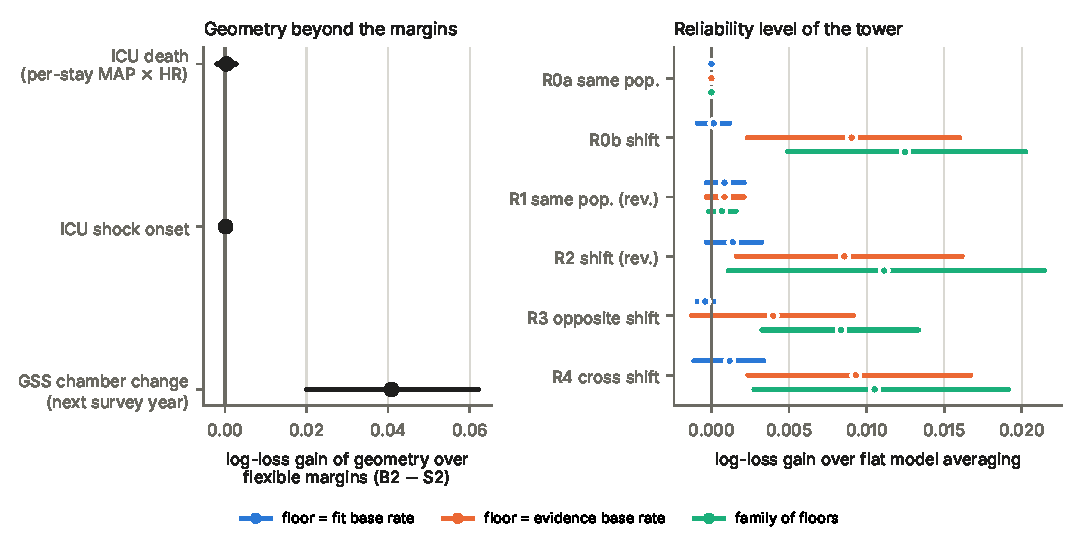
\includegraphics[width=\linewidth]{figs/fig_phase4.pdf}
\caption{Left: test log-loss gain of geometry over a flexible function of the margins, with $95\%$ intervals, for ICU death, ICU shock
onset and GSS chamber changes. Right: gain of each reliability level of the tower over flat model averaging in the six arms of
\cref{tab:gentower}.}\label{fig:phase4}
\end{figure}

%=====================================================================
\section{The context-to-outcome map, and geometry at the boundary}\label{sec:contextmap}
%=====================================================================

Several systems in this paper carry the same information in several contexts:
\begin{itemize}[leftmargin=*,nosep]
\item one spending item in two wordings;
\item one pressure band in four kinds of unit;
\item one question under two prompts.
\end{itemize}
The natural object is a map from (context, information) to a probability of an outcome, and the natural question is whether it depends
on the context. Algebraic geometry states this exactly. With context $C$, information $A$ and outcome $O$, \emph{context invariance}
$P(O\mid A,C)=P(O\mid A)$ is the conditional-independence model $O\perp C\mid A$. It is a toric variety in the simplex of
$C\times A\times O$ tables, cut out by the binomials $p_{cao}\,p_{c'ao'}-p_{cao'}\,p_{c'ao}$. Its distance from the data, the divergence
of the information projection, is $I(O;C\mid A)$, and twice the sample size times it (in nats) is the $G^2$ test. When invariance fails,
the binomials say where: at which level of the information the context changes the outcome map. The plan, its planted checks and
frozen results are in \texttt{ext/phase5}. The planted check held its size ($12$ rejections in $200$) and located a planted change at
the right answer level.

\paragraph{GSS: wording, answer and party.} Wording is randomized, so here a failure of invariance is a causal effect of the wording on
what an answer means politically.
\begin{itemize}[leftmargin=*,nosep]
\item \emph{Seven items are invariant.} For race, drugs, education, environment, space, defense and foreign aid, the wording changes how people answer but not what their answer says about their party.
\item \emph{Four items are not} (Bonferroni over eleven): welfare (mean $0.0126$ bits per year), crime, cities and health.
\item \emph{Where welfare fails.} The failure sits at ``about right'' ($58\%$ of its $G^2$). Saying welfare spending is about right is a
  different political statement from saying assistance to the poor is about right.
\end{itemize}
The toric decomposition makes this geometric (\cref{fig:contextmap}, right).
\begin{itemize}[leftmargin=*,nosep]
\item The answer $\times$ party coupling polytope of welfare has a different toric type in the two wordings in $23$ of $24$ years:
  usually $18$ vertices for ``welfare'' and $12$ or $15$ for ``assistance to the poor''.
\item In $16$ of those $23$ years the invariant map reproduces both types. There the change of toric surface is carried by the answer
  margins alone, as direct influence.
\item In the other $7$ the context changes the geometry through the outcome map itself.
\item No welfare chamber is decided on the bands in both wordings in any year. The toric types are point estimates, while the invariance
  test, which does not depend on the chamber, is decisive.
\end{itemize}

\paragraph{ICU: unit type, first-window pressure and death.} Invariance fails in both sets ($G^2=119$ and $141$ on $9$ df;
$0.022$ and $0.026$ bits). Its geometry shows how.
\begin{itemize}[leftmargin=*,nosep]
\item In cardiac surgery the observed death $\times$ pressure system is $\mathbb{CP}^2$, while the invariant map would make it
  $\mathbb F_1$. In set~B that chamber is decided on the bands.
\item In medical units it is the reverse.
\item The reason is that the death rate given borderline pressure is $2$--$3\%$ after cardiac surgery and $21\%$ in medical units.
  The same reading means different things in different units, and the Fano surface of the unit's system records it.
\end{itemize}

\begin{figure}[!htbp]
\centering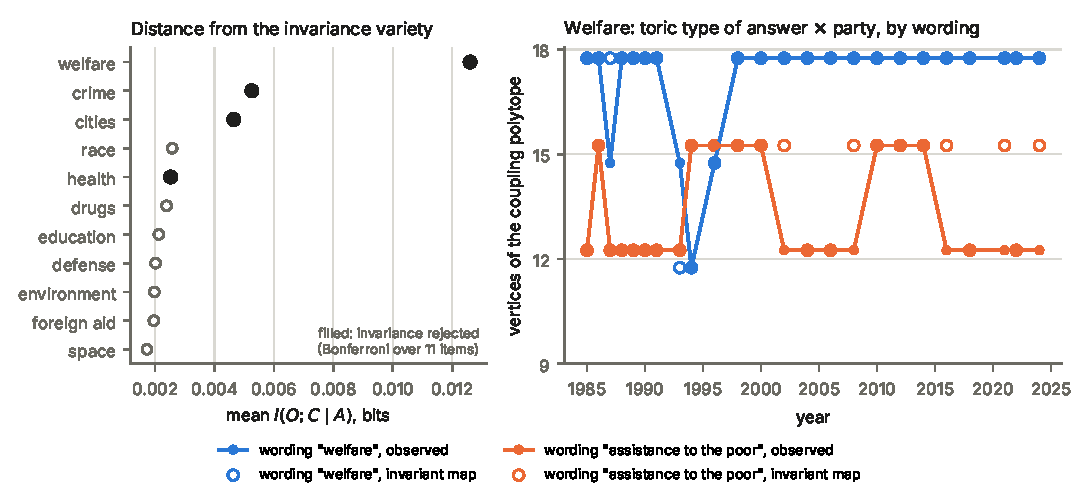
\includegraphics[width=\linewidth]{figs/fig_context_map.pdf}
\caption{Left: distance of each GSS item's wording $\times$ answer $\times$ party table from the invariance variety $O\perp C\mid A$ (mean
over $24$ years); filled when invariance is rejected. Right: toric type of the welfare answer $\times$ party system in each wording,
observed (lines) and under the invariant map (circles).}\label{fig:contextmap}
\end{figure}

\paragraph{Geometry at the boundary.} Per-stay ICU day systems usually have an empty band, and half have a point polytope
(\cref{sec:forecast}). A genuine point polytope carries no coupling information: when a margin is a single category the coupling is
fixed. That is a theorem, not a failure of the method. But most of these points are not genuine. A band with no hours in $22$ is a
zero count, not a zero probability. We re-ran the forecast of death with three boundary-aware readings:
\begin{itemize}[leftmargin=*,nosep]
\item the Dirichlet posterior over toric types;
\item the walls decided on the bands, i.e.\ the family over the band, which is a full-dimensional polytope \cite[Prop.~6.1]{Bands};
\item the face stratum, the torus orbit in which a broken system lies.
\end{itemize}
What the readings recover:
\begin{itemize}[leftmargin=*,nosep]
\item $71\%$ of day-two systems put more than half their posterior mass on full-support toric types, mostly the $12$-vertex type.
\item On average $8.7$ of the $18$ walls are decided.
\item The point polygons are therefore largely an artefact of the point estimate, and the geometry behind them is recoverable.
\end{itemize}
It still does not forecast death beyond a flexible function of the margins: gain $-0.0014$, interval $(-0.0052, 0.0023)$. The planted
check showed why such tests are hard: averaging over the posterior makes the geometric features smooth in the counts, so a flexible
margin model approximates them. The first planted check, with a weaker effect, could not detect it; it was replaced before the run by a
stronger one matched to the data, which did. So the boundary is not a dead end for the geometry. For this outcome, at this resolution, it
is a dead end for prediction.

%=====================================================================
\section{Tracking the approach to collapse: a family of cones, and recursive training}\label{sec:collapse}
%=====================================================================

A trajectory of systems traces a path of margins. Over a path, the coupling polytopes form a family whose union is again a polytope
\cite[Prop.~6.1]{Bands}, and each member's normal fan (a cone at each vertex) changes only where the path meets a wall. The walls
$f(I)=g(J)$ form the chamber complex of the marginal map. So the approach to collapse can be read off the path:
\begin{itemize}[leftmargin=*,nosep]
\item a \emph{bend} keeps the fan;
\item a \emph{tear} crosses a wall, and the fan gains or loses a cone: a blow-up or blow-down (for $2\times3$ systems, of a toric surface);
\item a \emph{break} reaches the boundary, and the fan drops dimension.
\end{itemize}
We built a tracker that reports, at every step of any trajectory:
\begin{itemize}[leftmargin=*,nosep]
\item the chamber, with signed wall distances and their band intervals;
\item tear and break margins, velocity, and tear and break times \cite[Def.~3.1, Thm.~3.2, Def.~5.7]{Bands};
\item the drift $D(p_t\Vert p_{t-1})$, split exactly by Csiszár's Pythagorean identity into \emph{interaction drift} $D(p_t\Vert p^*)$
  and \emph{margin drift} $D(p^*\Vert p_{t-1})$, with $p^*$ the I-projection of $p_{t-1}$ onto $p_t$'s margins;
\item the normal-fan type: dimension, vertices (maximal cones) and facets (rays);
\item a Dirichlet posterior over chambers.
\end{itemize}
Margin drift says who carries which information; interaction drift says what the information means. The plan
(\texttt{ext/phase6/PREANALYSIS\_COLLAPSE.md}) was fixed before anything was computed. Its planted checks passed:
\begin{itemize}[leftmargin=*,nosep]
\item the Pythagorean identity to $3\times10^{-13}$;
\item fan types against the existing toric code;
\item a planted wall crossing found at the right step;
\item a planted break detected.
\end{itemize}
Two checks had their specifications corrected before any real run. One rank-tolerance bug, which reported a dimension of $5$ for some
$3\times3$ systems, was found in the first trajectory run; it was fixed, a dimension check was added, and all trajectories were rerun.

\subsection{Five trajectories}
\begin{itemize}[leftmargin=*,nosep]
\item \emph{GSS, $110$ item-pair systems over $40$ years.} Across $2{,}530$ steps the fan is unchanged in $1{,}824$, blows up in $356$ and
  blows down in $350$. Only $18$ steps carry a decided chamber change. The run-up to the decided welfare $\times$ race tear (wording Y,
  2014$\to$2016) is visible in advance (\cref{fig:collapsetraj}, top left):
  \begin{itemize}[nosep]
  \item the tear margin shrinks from $0.018$ (2010) to $0.013$ (2012) and $0.006$ (2014);
  \item the tear time falls to $0.09$ steps, the smallest since 2008, when the path passed within $0.0002$ of a wall and the point fan dipped to $12$ vertices without any decided change;
  \item the posterior probability of the modal chamber drops to $0.48$ in 2014;
  \item interaction drift peaks in 2012 ($0.031$ bits, against a median of $0.006$);
  \item after the tear the chamber is decided ($0.99$) and the fan has lost three cones ($15\to12$).
  \end{itemize}
\item \emph{C19PRC waves.} Depression $\times$ anxiety keeps the same $15$-vertex fan through all waves in both countries. It sits very
  close to a wall (UK tear margin $0.0005$--$0.013$) without a decided change.
\item \emph{The tower's evidence paths.} Hypothesis change is motion through chambers. In the two shift arms with a mortality rise
  (R0b, R2), the level-one prediction crosses the wall $f_1=g_0$ twice as evidence accrues, and the fan alternates between
  $\mathbb{CP}^2$ and $\mathbb F_1$. In the same-population arm and in R4 it stays in one chamber.
\item \emph{ICU decedents against survivors.} In $6$-hour windows over $48$ hours, the decedents' pressure $\times$ heart-rate system
  hugs a wall after the first window: tear margin $0.001$--$0.018$, against $0.020$--$0.046$ for survivors. It keeps a $15$-vertex fan,
  where the survivors' drops to $12$ after the first window. Neither group approaches the boundary (break margins about $0.04$--$0.06$). The two groups, the same
  information in two outcome contexts, differ by $0.05$--$0.08$ bits per window, of which $88$--$98\%$ is margin drift.
\item \emph{LLM retraining (two points).}
  \begin{itemize}[nosep]
  \item Happy numbers and ARC \emph{break}: the fan drops dimension because a category empties.
  \item HotpotQA \emph{blows up} ($9\to12$ vertices).
  \item Primes makes four decided wall crossings with the same fan.
  \item In every task the drift is overwhelmingly in the margins (up to $3.4$ bits), with interaction drift $0.003$--$0.04$ bits.
  \end{itemize}
\end{itemize}

\begin{figure}[!htbp]
\centering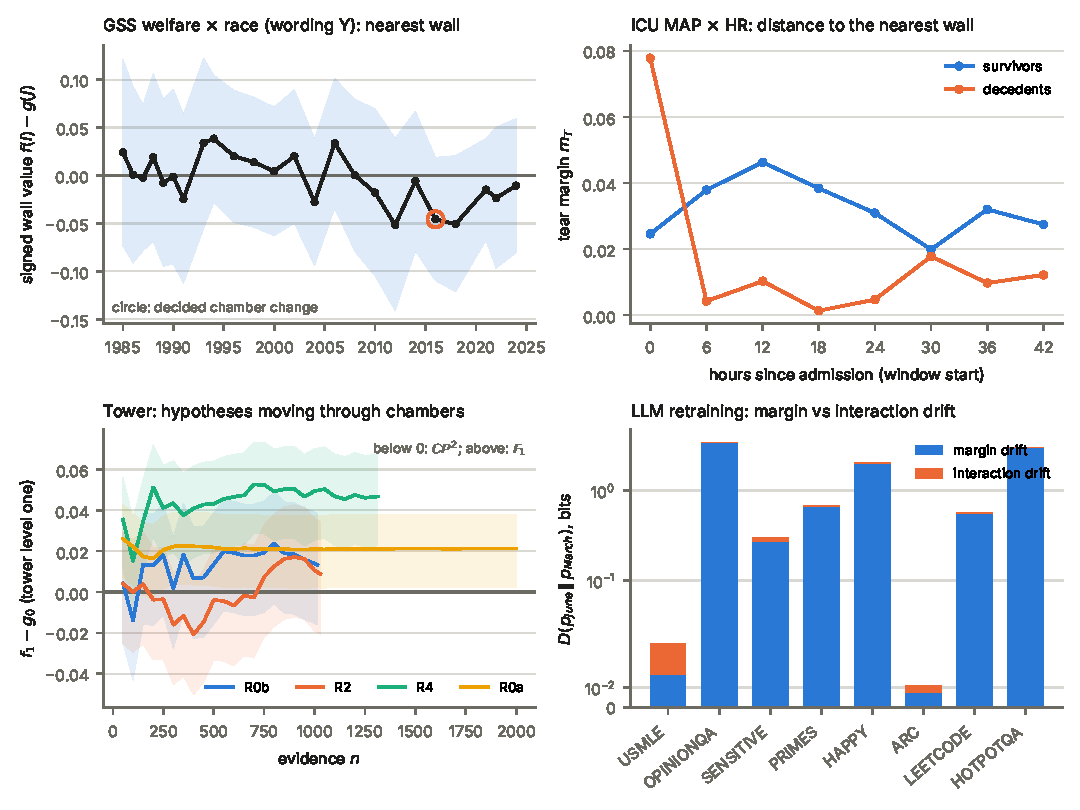
\includegraphics[width=\linewidth]{figs/fig_collapse_trajectories.pdf}
\caption{The tracker on four trajectories. Top left: the GSS welfare $\times$ race system (wording Y), signed value of the wall
nearest in 2014 with its band interval; the circle marks the decided chamber change. Top right: tear margin of ICU pressure $\times$
heart-rate systems in $6$-hour windows, decedents and survivors. Bottom left: the tower's level-one paths relative to the wall
$f_1=g_0$, with the interval from the pressure band. Bottom right: the March-to-June drift of the LLM systems split into margin and
interaction parts (bits, symmetric log scale).}\label{fig:collapsetraj}
\end{figure}

\paragraph{The forecasting test.} Does interaction drift, or tear time, forecast the next \emph{decided} chamber change beyond plain
margin velocity? The test set has only $11$ such events, below the pre-registered minimum of $15$. The test is underpowered, and
neither predictor adds anything: gains $-0.0001$, with intervals spanning $0$. On the secondary target, point-estimate chamber changes
($634$ test events):
\begin{itemize}[leftmargin=*,nosep]
\item tear time adds $0.017$, with an interval $(-0.001, 0.033)$ just touching $0$;
\item tear time with interaction drift adds $0.017$, $(0.0002, 0.034)$;
\item interaction drift alone adds nothing.
\end{itemize}
So distance to the walls carries the forecast, while the meaning-change part of the drift does not, at least not for the GSS.

\subsection{Recursive training with known truth}\label{sec:recursive}

\paragraph{Design.} A model of an outcome $y$ (eight values) given information $x$ (six values) in three contexts was retrained on its
own samples for $20$ generations: $200$ samples per cell, $50$ replicates. The truth satisfies context invariance, and some outcome
categories are rare tails. Fresh real data were mixed in at $0$, $5$, $10$ and $25\%$; a variant passed each generation through a
paraphrase kernel. Five predictions were fixed in advance; two hold and three fail (\cref{fig:recursive}).
\begin{enumerate}[leftmargin=*]
\item \emph{Contraction: holds, but trivially.} The paraphrase kernel's Dobrushin coefficient is $1$: it shifts outcomes to neighbours
  without mixing distant ones. The planned bound therefore reduced to ``no increase beyond noise''. The model's distinguishability of
  $x$ falls from $0.70$ to $0.24$ over $20$ generations, inside an exploratory sharper bound from the coefficients of the composite
  kernels $K^g$.
\item \emph{Breaks in finite time, forecast by break time: fails.}
  \begin{itemize}[nosep]
  \item Without fresh data, $88.5\%$ of tail categories are absorbed at zero by generation $20$, just short of the planned $90\%$; $36\%$
    are zero already in the model fitted to real data, a break caused by finite data alone.
  \item Break time correlates with the remaining time to the break (Spearman $0.33$), but the level alone does better ($0.48$).
  \item Given the level, break time adds nothing ($0.03$, $p=0.065$).
  \end{itemize}
\item \emph{Fresh data prevents absorbing breaks: fails as stated.}
  \begin{itemize}[nosep]
  \item Bands Prop.~9.2 guarantees a floor $\lambda P_0$ for the training law, not for a model fitted to $200$ samples.
  \item Categories rarer than about $1/(\lambda\cdot200)$ are zero most of the time whatever $\lambda$ is: $29$--$38\%$ of tracks have
    three consecutive zeros with fresh data, against $44\%$ without.
  \item Exploratory: the qualitative claim holds. Without fresh data a zero never recovers; with fresh data zeros recover at $7$--$19\%$
    per generation, and persistent zeros fall from $37\%$ to $16$, $11$ and $5\%$.
  \end{itemize}
\item \emph{Contexts drift off the invariance variety: holds, decisively.}
  \begin{itemize}[nosep]
  \item Without fresh data, the model's $I(Y;C\mid X)$, its distance from the toric variety $Y\perp C\mid X$, grows steadily from
    $0.016$ to $0.18$ bits, in every replicate.
  \item With fresh data it plateaus at $0.09$, $0.058$ and $0.03$ bits for $5$, $10$ and $25\%$.
  \item Retraining contexts on their own outputs makes the same information mean different things in different contexts. That is
    the ``bogus information'' of the question, measured exactly, and fresh data cap it.
  \end{itemize}
\item \emph{Certificates warn before accuracy drops: fails.}
  \begin{itemize}[nosep]
  \item The tower-style certificate against held-out real data (the distance to the held-out band plus the Cromwell mass the model has
    zeroed) rises steadily from the first generation.
  \item But accuracy also falls from the first generation, and its first $5$-point drop comes at a median generation of $2$ (range $1$--$10$).
  \item The certificate crosses its null threshold strictly first in $58\%$ of replicates, short of the planned $80\%$; the median lead
    is $2$ generations.
  \end{itemize}
\end{enumerate}

\begin{figure}[!htbp]
\centering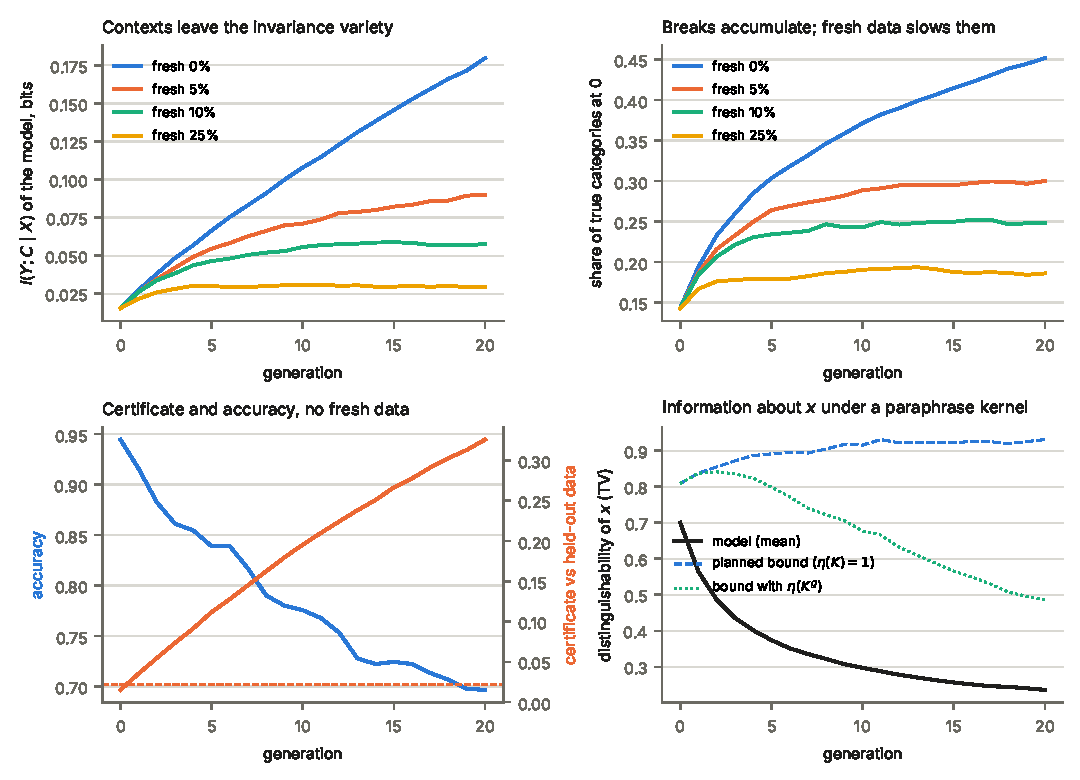
\includegraphics[width=\linewidth]{figs/fig_recursive.pdf}
\caption{Recursive training with known truth ($50$ replicates). Top left: the model's distance from the context-invariance variety,
$I(Y;C\mid X)$, by fresh-data share. Top right: share of true outcome categories the model has at zero. Bottom left: mean accuracy and
mean certificate against held-out real data without fresh data; the dashed line is the certificate's null threshold. Bottom right:
distinguishability of the information under a paraphrase kernel, with the planned and the sharper bound.}\label{fig:recursive}
\end{figure}

\paragraph{What this shows.} The tracker turns any trajectory into a sequence of chambers, fans and drifts, and on real data it shows
approach to a wall before a tear. It did so for welfare $\times$ race, for the decedents' physiology, and for the tower's hypotheses.
In recursive training, the clearest signal of information being destroyed is not the loss of tails, which finite data cause from the
start. It is the steady departure of the contexts from the invariance variety. That departure has no counterpart in accuracy and is
invisible to any single-context metric, and fresh data bound it in proportion to their share. What did not work as predicted:
\begin{itemize}[leftmargin=*,nosep]
\item break time as a forecaster beyond the level;
\item Prop.~9.2 as a finite-sample floor;
\item the certificate as an early warning with a large lead.
\end{itemize}
Each needs a sharper statement or a longer horizon, and the analysis does not go beyond these results.

%=====================================================================
\section{Ambient support geometry: deciding under uncertainty with floors, typed obstructions and replayable records}\label{sec:support}

The tracker of \cref{sec:collapse} describes; a decision has to be made from it. This section integrates the proposal
\emph{Ambient Support Geometry: Presheaves, Positive Support Floors, and Local-to-Global Obstructions} \cite{SupportAmbience} into the
programme, sharpens it where the data and the mathematics allow, replaces its comonadic layer by a fibred, locally posetal
2-category, and reports a pre-registered test of its experimental programme (\texttt{ext/phase7}, plan
\texttt{PREANALYSIS\_SUPPORT.md}, hash frozen before any experiment; code hashed before the run).

\subsection{Support as a policy, and the local-first principle}
A probability model normally lets a coordinate approach zero. In applications the question is often not whether an outcome is
possible, but whether it has enough support to be relied on: a rare event may be possible and still too weakly supported for a
particular decision, while a strict floor can be wrong when rare but real outcomes must be kept. The threshold therefore belongs
to the ambient decision context, not to probability alone. Following the proposal, a decision combines four pieces of information:
\begin{enumerate}[leftmargin=*,nosep]
\item a \emph{support policy}: which outcomes or events must have probability at least a chosen floor;
\item the \emph{local probability geometry}: margins, conditionals and coupling constraints;
\item \emph{provenance}: which observations, assumptions and policy choices led to the decision;
\item an \emph{obstruction signature}: the weakest support margin, and any local-to-global or composition failure.
\end{enumerate}
The aim is not to force every local structure into a global model, but to make each local conclusion auditable and to expose
where the chain from evidence to outcome becomes fragile. A global emergent object may not exist, or may exist only under
assumptions the evidence does not justify; so a global model is not the default data structure. Each context carries its own
local probability object, policy and evidence trail; restriction says what remains visible in a smaller context; compatibility
asks whether local objects agree on overlaps; gluing asks whether compatible local objects come from one global object. This is the
use-case for a presheaf $F:\mathcal C^{\mathrm{op}}\to\mathbf{Set}$ (or to constraint objects or records), with restriction maps
$\rho^U_V:F(U)\to F(V)$ for $V\subseteq U$. A presheaf asserts no global section; in an AMB measurement scenario a compatible family
that fails to extend is a contextuality witness, meaningful precisely because local compatibility does not force a global section
\cite{AbramskyMansfieldBarbosa2012}.

\subsection{Floors and the coupling polytope}
For margins $f\in\Delta(X)$, $g\in\Delta(Y)$ and floors $\tau\ge0$ on a set $D$ of designated cells, the support-constrained polytope is
\begin{equation}\label{eq:Ptau}
P_\tau(f,g)=\{\pi\in P(f,g):\pi_{xy}\ge\tau_{xy}\text{ for }(x,y)\in D\};
\end{equation}
more generally one may floor events, $\pi(E_k)\ge\tau_k$.

\begin{remark}[Two thresholds]\label{rem:thresholds}
A floor has probability units, $0\le\tau\le1$. A safety factor such as ``$1.1$'' is dimensionless: relative to a baseline floor
$\tau^{(0)}$ it means $\tau\ge1.1\,\tau^{(0)}$; it is not a probability of $1.1$. The decision layer below also uses a \emph{relative}
threshold $\kappa$ between competing actions, $q_x\ge\kappa q_y$: the wall $q_x=q_y$ replaced by the binomial $q_x=\kappa q_y$. A
multiplicative constant keeps the binomial form (a translate of the toric variety); an additive one, $p^u-p^v=c$, does not. Both
thresholds are implemented and kept apart.
\end{remark}

\begin{proposition}[Feasibility is policy-relative \cite{SupportAmbience}]
$P_\tau(f,g)$ is a possibly empty polytope. If it is empty, the margins and the policy cannot hold together; this does not by itself
make the data false: the floor may be too strong, the margins uncertain, or the cells unsuitable for a common guarantee.
\end{proposition}

The proposal cautions that truncation ``need not preserve the original toric fan''. For floors on cells it does, exactly:
\begin{proposition}\label{prop:reducedmargins}
Let $f'=f-\tau\mathbf 1_D\mathbf 1$ and $g'=g-\mathbf 1^\top\tau\mathbf 1_D$ be the reduced margins. Then
$\pi\mapsto\pi-\tau\mathbf 1_D$ is a bijection from $P_\tau(f,g)$ onto $P(f',g')$. Hence $P_\tau$ is non-empty iff $f',g'\ge0$; its
normal fan is that of $P(f',g')$; its walls are $f'(I)=g'(J)$; and the largest common margin above the floors with weights $w$,
\begin{equation}\label{eq:headroom}
\delta^\star=\max\{\delta:\pi\in P(f,g),\ \pi_{xy}\ge\tau_{xy}+w_{xy}\delta\ \text{on }D\},
\end{equation}
equals $\min$ over rows and columns of (margin $-$ floors)/(weights) whenever that value is non-negative, with a row or a column as
the bottleneck.
\end{proposition}
\begin{proof}On $D$, $\pi\ge\tau$ is $\pi-\tau\mathbf 1_D\ge0$; off $D$ the shift is zero; the margins shift by the row and column sums
of $\tau\mathbf 1_D$. A transportation polytope with non-negative margins of equal total is non-empty. For \eqref{eq:headroom} apply
the same shift with $\tau+w\delta$; it is valid while $\tau+w\delta\ge0$.\end{proof}
So a floor alone can cross a wall: a policy can tear a system. On the uniform $2\times3$ hexagon a floor on one cell crosses two walls at $\tau=\tfrac16$ and breaks the system at $\tau=\tfrac13$ \cite[Ex.~6.10]{Conditionals}. Floors on events give general polytopes, and the proposal's caution
applies to them. The support obstruction for cell floors needs no optimisation: its certificate reads ``this row carries $f_x$, but
its floors demand more''; with margins known only to their bands, a floor is decided-feasible when the lower band ends cover the
floor sums. The weakest link is kept as a typed signature, not a single score,
\[
\mathfrak O=(\mathfrak O_{\mathrm{supp}},\mathfrak O_{\mathrm{glue}},\mathfrak O_{\mathrm{comp}},\mathfrak O_{\mathrm{evid}}),
\]
recording support shortfall, failure to glue, failure to compose and inadequate or conflicting evidence. Its components have
different mathematical types, and combining them requires an explicit normalisation and decision policy.

\subsection{Chains, presheaves, and two vocabularies kept apart}
The proposal's ``spring leaf'' is a \emph{local constraint chain}: a path of contexts $U_0\leftarrow U_1\leftarrow\cdots\leftarrow U_n$
with local states $s_i\in F(U_i)$, restriction or transport maps between them, and a support slack and obstruction recorded at each
stage. A conclusion is carried forward only while the compatibility conditions hold; when they fail, the chain records where and
why, instead of inventing a global state. A chain follows one route; a presheaf records all routes, and two routes that transport
a conclusion differently give a path-dependence (holonomy) diagnostic \cite{HolonomyNote}.

Two vocabularies are used side by side. On the AMB side \cite{AbramskyMansfieldBarbosa2012}, a measurement scenario has contexts and
an assignment presheaf, and a compatible family that fails to extend is a contextuality witness. On Vigneaux's side
\cite{Vigneaux2019,BaudotBennequin2015}, an information structure has observables with a conditioning action, and information
functionals such as entropy live there. The support ambience attaches floors, bands, provenance and obstruction records to each
context, which enriches the local data but does not identify the two coefficient systems. In particular the support indicator
(positive section $\mapsto1$, empty $\mapsto0$) is not additive, so it is not a morphism of abelian coefficient systems and induces
no map of cohomologies; nor does a holonomy cocycle of known transformations become the AMB obstruction because both are local. The
division of labour is: the presheaf says what local states exist and how they restrict; the floored polytope, which assignments
meet the constraints; the conditioning action, how information functionals respond to conditioning; the AMB extension test,
whether compatible support sections extend \cite{Vorobev1962}; provenance, which evidence and policies produced the result.

\subsection{Carrying the ambience: a fibred, locally posetal 2-category}\label{sec:fibred}
The proposal carries the ambient record $a=(m,\tau,\mathcal E,\mathcal G,\mathcal D)$ (constraints, floors, evidence, gluing rules,
decision policy) by an informal comonad $C_a(Y)=Y\times A_a$, and leaves its laws and its transport rule open. The programme already
carries the tower's context in the way this asks for. Over each finite base $B$ the context sits in a reader comonad
$\mathsf C^B(Y)=Y\times A_B$; every Markov kernel $k$ transports it by a comonad morphism $\mathrm{id}\times A_k$, functorially on
the Kleisli category \cite[Prop.~9.14]{Tower}; and the category of elements of $B\mapsto A_B^{\mathrm{coh}}$ is a split
opfibration over the Kleisli category, along whose lifts the comonads are carried \cite[Prop.~3.3]{Conditionals}, certificates pull
back and failure levels can only rise \cite[Thm.~3.1]{Conditionals}. So the proposal's comonad, read correctly, is that family:
one comonad per context, carried along transports. What the ambience adds is \emph{order}: the fibres of the existing opfibration are
sets of points (coherent contexts), and a support policy needs sets of laws ordered by strength. The construction below is the
posetal enlargement of the existing one; its laws are immediate, and its content is the transport rule.

\begin{definition}[Ambience functor and its total category]\label{def:ambience}
Let $\mathcal C$ have contexts as objects and transports as morphisms $t:U\to V$: marginalisations (restriction to fewer
variables), deterministic maps and Markov kernels $K_t$ on cells. Let $\mathcal A(U)$ be the poset of closed convex feasible sets
$S\subseteq\Delta(X_U)$ (credal sets, floored polytopes), each carrying its record, ordered by inclusion: $S\le S'$ if $S\subseteq S'$,
so an arrow is a \emph{weakening}. Transport acts by images, $t_!S=K_tS$. The ambience's total category $\int\!\mathcal A$ (its
Grothendieck construction \cite{MacLaneMoerdijk1992,Johnstone2002}) has objects $(U,S)$ and an arrow $(U,S)\to(V,S')$ for each
$t:U\to V$ with $t_!S\subseteq S'$. The projection $\pi:\int\!\mathcal A\to\mathcal C$ is an opfibration whose fibres are posets.
Restricted to kernels and to singletons $S=\{\rho\}$ at level one, it is the level-one part of the discrete opfibration of
\cite[Prop.~3.3]{Conditionals}.
\end{definition}

\begin{proposition}\label{prop:fibred}
\begin{enumerate}[leftmargin=*,nosep]
\item Images compose strictly, $(st)_!=s_!t_!$, so $\mathcal A:\mathcal C\to\mathbf{Pos}$ is a functor. A decision is a path in
  $\int\!\mathcal A$; its replay is the composite, which depends only on the recorded path.
\item Imposing a policy, $\iota_\tau(S)=S\cap\{\pi\ge\tau\}$, is an idempotent comonad on each fibre (an interior operator:
  $\iota_\tau S\subseteq S$, $\iota_\tau\iota_\tau=\iota_\tau$); summarising a set by its floors,
  $\sigma(S)=\{\pi\in\Delta:\pi\ge\min_S\pi\}$, is an idempotent monad (a closure operator: $S\subseteq\sigma S$, $\sigma\sigma=\sigma$).
  The counit, comultiplication and unit laws hold trivially in a poset.
\item Neither commutes with transport, and the failures point one way:
  $t_!\,\iota_\tau S\subseteq t_!S\cap\{\pi\ge K_t\tau\}$ and $\sigma\, s_!\,\sigma\, t_!S\supseteq\sigma\,(st)_!S$. Imposing a policy
  before transport certifies at least as much as pushing the floor forward; summarising between steps certifies at most as much
  as carrying the set. Each inclusion is a 2-cell: on floor boxes, $t\mapsto\sigma\circ t_!$ is a normal oplax functor into posets
  \cite[Prop.~10.24]{Tower}.
\item On a discrete (op)fibration (a $\mathbf{Set}$-valued ambience, whose fibres have only identity arrows) every fibred comonad is
  the identity: a counit $c(a)\to a$ inside a discrete fibre forces $c(a)=a$. This is why the programme carries comonads
  \emph{alongside} its discrete opfibration, as a family $\mathsf C^B$ joined by comonad morphisms, and not \emph{on} it.
\end{enumerate}
\end{proposition}
\begin{proof}(1) $K_sK_t=K_{st}$, and the composite of a path is determined by its arrows. (2) Intersection with a fixed set and
taking the floor box are deflationary-idempotent and inflationary-idempotent; in a poset every such operator is a comonad,
respectively a monad. (3) If $\pi\in S$ and $\pi\ge\tau$ then $K_t\pi\in K_tS$ and $K_t\pi\ge K_t\tau$, since $K_t\ge0$; and
$\sigma t_!S\supseteq t_!S$ gives $s_!\sigma t_!S\supseteq(st)_!S$, then apply the monotone $\sigma$. (4) Immediate.\end{proof}

So the structure is a 2-category fibred over the contexts and \emph{locally posetal}: 0-cells are contexts with their feasible
sets, 1-cells are transport laws (the image $t_!$, the naive pushed floor $K_t\tau$, the tight floor $\min_{t_!S}$), and 2-cells are
inclusions between them. The naive floor sits below the tight one: in the pre-registered transport experiment (E5 below) the two
agree for only $27\%$ of target cells. In an exploratory run of $300$ random two-step chains (\texttt{lax\_composition.py}) the
stepwise-summarised floor fell strictly below the composite floor in $611$ of $895$ target cells and never above it, and imposing
the policy first certified strictly more than the transported floors combined with the pushed floor (their componentwise
maximum) in all $1{,}158$ cells. The consequence for the weakest
link is precise: carrying sets, transport loses nothing; certification is lost where a set is summarised by floors, or where a
policy is pushed forward instead of imposed. Along a whole leaf-spring chain of transports and vertical steps this becomes a
theorem \cite[Thm.~10.26]{Tower}: certification is path-independent, it is lost only at summaries and weakenings, the loss splits
exactly into non-negative contributions, one per summary, and imposing early and summarising late certifies most. The proposal's intuition of a comonadic layer survives in this modest form, policy
imposition as an interior operator on each fibre, while its open obligation, the transport law, becomes the oplax comparison of
\cref{prop:fibred}(3), which can be computed. The ordered total category and its floors are now part of the theory papers
\cite[Def.~3.5, Prop.~3.6]{Conditionals}, \cite[Section~10.7]{Tower}. The ambience is deliberately a \emph{prestack}, not a stack: descent is not imposed,
because the failure of descent is the information.

\paragraph{Why not other ways.} Each alternative below was considered and rejected for the stated reason.
\begin{center}\small
\begin{tabular}{>{\raggedright\arraybackslash}p{0.27\linewidth}>{\raggedright\arraybackslash}p{0.66\linewidth}}
\toprule
Alternative & Why not, or what it is good for\\
\midrule
Product (reader) comonad $Y\times A$ & Used, not rejected: it is the tower's per-base comonad $\mathsf C^B$, carried along kernels by comonad morphisms \cite[Prop.~9.14]{Tower}. With one fixed parameter, as in the proposal's $Y\times A_a$, it cannot follow a change of context and keeps no history.\\
Fibred comonad on $\int\!A$, $A$ set-valued & Trivial by \cref{prop:fibred}(4): discrete fibres admit no non-identity counit; hence the family of comonads above.\\
A general (non-posetal) 2-category, natural transformations as 2-cells & Coherence obligations without content: the fibres are posets of feasible sets, so 2-cells are inclusions and every diagram of 2-cells commutes. The quantitative counterpart is the graded shadow of \cite[Thm.~7.8]{Attribution}, a strict 2-category enriched in Lawvere metric spaces; with couplings as 2-cells the witness layer is neither a 2-category \cite[Thm.~7.6]{Attribution} nor a double category, strict or lax \cite{Algebras}. The oplax comparison here is of a functor into posets, not of those layers.\\
Sheaf or stack & Imposes descent, i.e.\ that compatible families glue; here the failure to glue is the datum to be recorded.\\
Topos and internal logic & Not needed: support is graded by headroom, not by truth values, and nothing uses a subobject classifier.\\
A single global model (Bayesian network, global joint) & Presupposes the global section whose existence is in question.\\
Writer monad (an append-only log) & Records history but not what restriction means; it is how the records are stored (\texttt{support.record}), not the mathematics.\\
Markov category \cite{Fritz2020} & The natural home for the 1-cells (composing kernels); it carries neither policies nor gluing data, and can serve as $\mathcal C$.\\
A scalar confidence score & Flattens the four obstruction types; a shortfall, a Farkas vector, a holonomy and a lying source are different evidence.\\
A cohomology map AMB $\to$ Vigneaux & Blocked: the support indicator is not additive (above).\\
\bottomrule
\end{tabular}
\end{center}

\begin{figure}[!htbp]
\centering
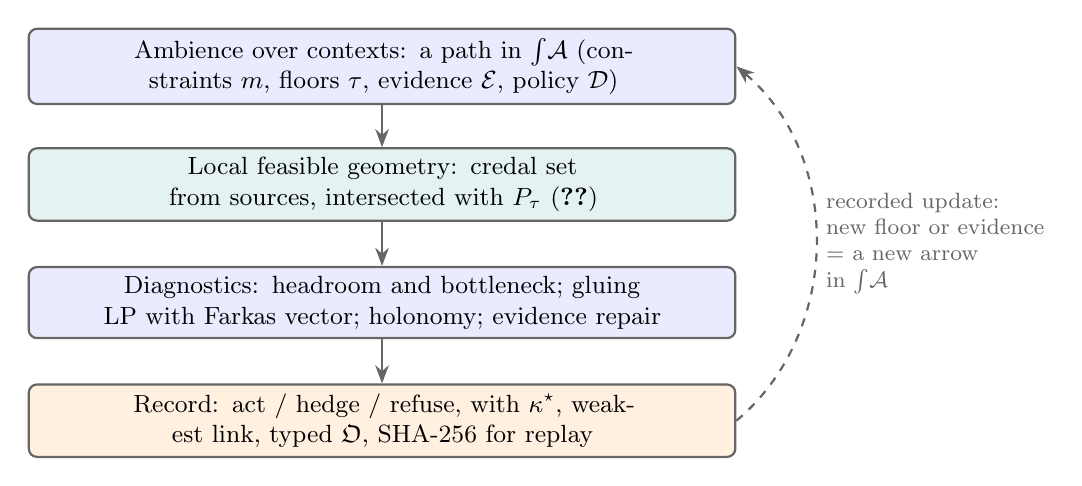
\begin{tikzpicture}[blk/.style={draw=black!60,rounded corners=3pt,thick,minimum width=0.74\linewidth,text width=0.72\linewidth,minimum height=0.8cm,align=center,font=\small},
  arr/.style={-{Stealth[length=2.3mm]},thick,black!60},every node/.style={font=\small}]
  \node[blk,fill=blue!8] (amb) at (0,4.5) {Ambience over contexts: a path in $\int\!\mathcal A$ (constraints $m$, floors $\tau$, evidence $\mathcal E$, policy $\mathcal D$)};
  \node[blk,fill=teal!10] (poly) at (0,3.0) {Local feasible geometry: credal set from sources, intersected with $P_\tau$ (\cref{prop:reducedmargins})};
  \node[blk,fill=blue!8] (diag) at (0,1.5) {Diagnostics: headroom and bottleneck; gluing LP with Farkas vector; holonomy; evidence repair};
  \node[blk,fill=orange!12] (dec) at (0,0) {Record: act / hedge / refuse, with $\kappa^\star$, weakest link, typed $\mathfrak O$, SHA-256 for replay};
  \draw[arr] (amb)--(poly); \draw[arr] (poly)--(diag); \draw[arr] (diag)--(dec);
  \draw[arr,dashed] (dec.east) to[bend right=50] node[right,align=left,font=\footnotesize]{recorded update:\\new floor or evidence\\$=$ a new arrow\\in $\int\!\mathcal A$} (amb.east);
\end{tikzpicture}
\caption{The decision architecture of \cite{SupportAmbience}, with its comonadic layer replaced by the total category of the ambience.
Feedback changes the ambience only through a recorded arrow, so every decision replays from its path.}\label{fig:architecture}
\end{figure}

\subsection{The decision layer}
\paragraph{Sources, reliabilities and the credal set.} Each source $c$ reports counts over its own outcomes, with a reliability $r_c$
(or an interval, whose low end is used) and, where its context legitimately changes the outcomes, a known map $T_c$. Writing
$P_c=r_cT_cq+(1-r_c)F_c$ with $F_c$ unrestricted, the band of $P_c$ bounds the true outcome law $q$ from above and below; all sources
together give a polytope $Q$, intersected with the policy's floors. When the sources contradict each other $Q$ is empty, a regional
failure to glue: an elastic linear program names the conflicting sources and outcomes, every single exclusion that would restore
consistency is listed, and by default the least reliable of these is excluded, with the largest reliability its data allow recorded
($\mathfrak O_{\mathrm{evid}}$). A floor the sources cannot support is reported, with its shortfall and binding bounds, not imposed
($\mathfrak O_{\mathrm{supp}}$). Each decision is one linear program per pair of actions; the output carries the strength
$\kappa^*$, a trace that splits the worst-case margin exactly among the sources by duality, the binding bounds, the weakest link
(for each source, the reliability below which the decision fails), the thinnest cell, and which source's further data would help most.

\paragraph{A worked example (synthetic).} Three answers $a,b,c$; four sources: a reference text ($r=0.9$), a forum ($r=0.3$, whose
falsehoods push $c$), a paraphrase set ($r\in[0.6,0.7]$, pushing $b$), and self-generated text claiming $r=0.8$ but carrying no true
signal. The self-generated source is found to contradict the others (its data allow at most $r=0.03$) and is excluded. ``Assert $a$''
is then supported up to $\kappa^*=1.68$: the layer acts at $\kappa=1.1$ and $1.5$ and hedges between $a$ and $b$ at $\kappa=2$. The
decision does not depend on the reference text at all; it rests on the forum's upper bound on $b$ (the forum is mostly wrong but
rarely says $b$), so its weakest link is the forum, whose reliability must stay above $0.235$ (stated $0.3$) at $\kappa=1.1$.

\paragraph{A decision record.} The proposal's illustrative record, filled in from a real run (one register, $r=1$, counts
$600/300/100$ over $a,b,c$; policy: $c$ at least $0.30$):
\begin{center}\small
\begin{tabular}{>{\raggedright\arraybackslash}p{0.22\linewidth}>{\raggedright\arraybackslash}p{0.7\linewidth}}
\toprule
Field & Record\\
\midrule
Decision & Support obstruction: no action\\
Policy & $q_c\ge0.30$\\
Active constraint & the floor on $c$ (bottleneck)\\
Witness & the register's band forces $q_c\le0.125$ (dual $-1$ on its upper bound for $c$)\\
Weakest link & shortfall $0.175$\\
Provenance & source counts, reliabilities and policy version, hashed\\
Next action & revise the floor, revise the evidence, or defer\\
\bottomrule
\end{tabular}
\end{center}
With the floor at $0.05$ instead, the layer acts (``assert $a$'') with headroom $0.075$ on the floor, the same bound binding.

\subsection{Entropy, Fisher geometry and the three gluing statuses}
A floor changes the admissible region; it does not turn a toric equation into one with a positive constant (\cref{rem:thresholds}).
On the interior of the simplex, entropy and the Fisher metric are regular, and a floor keeps the floored coordinates away from the
boundary, which can only improve regularity on the constrained region; by \cref{prop:reducedmargins} cell floors keep the toric
type of the reduced margins, while the Fano property and the disc potential still have to be checked for each new polytope. For
gluing, with $(X,Y)$ and $(Y,Z)$ margins fixed, every filler satisfies $H(X,Y,Z)\le H(X,Y)+H(Y,Z)-H(Y)$, with equality exactly when
$X\perp Z\mid Y$. A floor can exclude this maximum-entropy filler while other fillers survive, so three statuses are kept apart: a
filler exists; a filler meets the policy; the maximum-entropy filler is among the admissible ones.

\subsection{The pre-registered programme}
The proposal's minimal experimental programme was pre-registered and run once; two checks failed as specified and are reported
with their corrections.
\begin{itemize}[leftmargin=*,nosep]
\item \emph{E1, floored geometry.} In $500$ random floored systems ($2\times2$ to $3\times4$, random designated cells), the vertices,
  enumerated independently, are the shifted vertices of the reduced-margin polytope in all $500$ (worst discrepancy $10^{-8}$), and
  the $2\times3$ toric surfaces agree in $84$ of $84$; all $200$ systems with a negative reduced margin are infeasible. As run, the
  check reported $324$ of $500$, because its comparator sorted rounded vertex lists, which is order-sensitive; the order-free
  comparison of the same instances is a reported deviation.
\item \emph{E2, weakest link.} The closed form of \cref{prop:reducedmargins} equals the linear program in all $418$ cases with
  headroom. The planned check on the duals failed ($82\%$ against $99\%$): duals on margin equalities are defined only up to adding a
  constant to the rows and subtracting it from the columns. The gauge-invariant version (the binding floors lie in the bottleneck
  row or column) holds in $418$ of $418$. Without headroom the closed form does not apply; it differs in $43\%$ of cases.
\item \emph{E3, the chain $X-Y-Z$} ($200$ binary instances, $20$ floors each). A floored filler exists iff $\tau\le\min\pi/2$ over the
  two given tables ($4{,}000$ of $4{,}000$). The conditional-independence filler meets the floor iff
  $\tau\le\tau_{CI}=\min_{x,y,z}\pi(x,y)\pi(y,z)/\pi(y)$, always the smaller threshold ($200$ of $200$), and the maximum entropy over
  admissible fillers attains the bound exactly when $\tau\le\tau_{CI}$ ($2{,}600$ of $2{,}600$). Between the two thresholds a
  floor-meeting filler exists, but not the least committal one.
\item \emph{E4, the cyclic cover} $(X,Y),(Y,Z),(Z,X)$. Gluability by linear program agrees with the $3$-cycle inequalities
  \cite{AraujoEtAl2013} in $600$ of $600$ families; all $81$ contextual families come with a Farkas vector, verified independently. Of
  the $519$ gluable families, $124$ ($24\%$) are \emph{support-contextual}: every local table meets its floor, the family glues, and
  yet no global section meets the floor. This is a new obstruction type, a recorded witness rather than a cohomology class. For the binary triangle it has a closed form: a floored global section exists iff every pairwise cell is at least $2\tau$ and the $3$-cycle inequalities hold with right side $1-8\tau$ \cite[Thm.~4.8]{Conditionals}, so support-contextuality is the band between those inequalities at $\tau$ and at $0$; the triangle with cells $000$ and $111$ empty and the rest $\tfrac16$ is support-contextual at every $\tau\in(0,\tfrac1{12}]$ \cite[Ex.~4.9]{Conditionals}.
\item \emph{E5, transport.} Floors push forward through any non-negative kernel: $\pi\ge\tau$ implies $K\pi\ge K\tau$ ($500$ of $500$).
  Under deterministic coarsening the slack of a state never shrinks ($250$ of $250$); under a stochastic kernel it stays above the
  smallest row sum of $K$ times the original slack ($250$ of $250$) and shrinks in $2\%$ of cases. The pushed floor is the tight one
  for $27\%$ of target cells: the 2-cell of \cref{prop:fibred} is usually not an identity.
\item \emph{E6, records.} All $400$ recorded decisions ($100$ problems, each through three changes of floor, evidence and $\kappa$)
  replay bit-identically from their records, and $20$ planted obstructions of each type are classified to that type alone ($80$ of
  $80$).
\end{itemize}

\subsection{Real retrieval data: SciFact}\label{sec:scifact}
SciFact \cite{Wadden2020} pairs $1{,}409$ expert-written scientific claims with $5{,}183$ abstracts, labelled SUPPORT, CONTRADICT or
not enough information (NEI) per claim--abstract pair. We used oracle abstracts: $919$ training pairs and $340$ dev pairs (gold
$138/71/131$); the unlabelled test split was not used. The sources are three weak classical verifiers trained on the training split.
Pretrained inference models could not be loaded here, so the sources are much weaker than modern ones, and every result below should
be read as a test of the decision layer under weak evidence. Two pre-registered analyses were run; the first comes from an earlier
branch of this work, and the second was planned without knowledge of the first's results.

\paragraph{Analysis 1: channels and credal rules} (\texttt{ext/scifact}, plan frozen before any model was fitted). Each verifier's
confusion channel, and their joint channel over the $27$ output patterns, were estimated by five-fold cross-validation on the
training split, with bands; credal rules assert a label when its lower posterior beats every rival's upper posterior by
$\kappa=1.1$.
\begin{itemize}[leftmargin=*,nosep]
\item Baselines: best single verifier $64.7\%$ accurate, majority vote $60.9\%$, naive Bayes $66.8\%$ (macro-F1 $0.61$).
\item The credal rule on the empirical joint channel acts on $21\%$ of pairs and is $88.7\%$ accurate when it acts, against naive
  Bayes's $66.8\%$ on all pairs: \emph{H1 holds} (difference $0.22$, interval $0.15$--$0.29$). The rule that assumes independent
  errors acts on $34\%$ at $86.2\%$; the rule with no dependence assumption (Fréchet bounds) never acts.
\item \emph{H2 fails}: the pairs on which the independence rule acts but the joint-channel rule does not were not measurably worse
  (difference $0.07$, interval $-0.07$--$0.21$, $45$ pairs).
\item \emph{H3 holds}: the strength $\kappa^*$ ranks correct above incorrect labels (AUC $0.59$, interval $0.53$--$0.66$).
\item \emph{H4 fails}, against the geometry: ranked by $\kappa^*$, the area under the risk--coverage curve is \emph{larger} than when
  ranked by naive Bayes's confidence ($0.249$ against $0.192$, interval of the difference $-0.088$ to $-0.028$).
\item Exploratory: at the same coverage the credal gate picks the same pairs as confidence thresholding ($71$ of $71$), and it only
  ever asserts NEI. Its hedges contain the gold label in $95\%$ (SUPPORT or NEI), $100\%$ (all three) and $91\%$ (SUPPORT or
  CONTRADICT) of cases. No dev claim with several abstracts produced a decided SUPPORT on one and a decided CONTRADICT on another.
\end{itemize}

\paragraph{Analysis 2: conformal reliabilities and the decision layer} (\texttt{ext/scifact/conformal}). Here each verifier's
reliability is the conformal quantile of the probability it gives the true label on a held-out calibration quarter of the training
split, at level $0.05/3$. Then the credal set of \cref{sec:support} contains the truth whenever every source covers it, and acting on a
wrong label is impossible at $\kappa\ge1$, so $P(\text{act and wrong})\le0.05$: a finite-sample guarantee, under exchangeability,
that needs no model of how the verifiers' errors depend on each other.
\begin{itemize}[leftmargin=*,nosep]
\item \emph{P1 holds}: no wrong act on dev; some source missed the truth on $3.5\%$ of pairs, within the $5\%$ bound.
\item \emph{P2 fails}, decisively: the reliabilities are $0.056$, $0.039$ and $0$, the credal set is nearly the whole simplex, and the
  layer acts on $4$ of $340$ pairs ($1.2\%$, all NEI, all correct).
\item \emph{P3 holds}: three sources act on $4$ pairs at the same guarantee where the best single source acts on $1$, and that one is
  wrong. \emph{P4 holds} only formally ($4$ pairs; interval $0$--$0.5$). \emph{P5 holds}: the best verifier is $47$ points more
  accurate on the pairs the layer acts on than on those it hedges (interval $0.41$--$0.52$).
\item Risk--coverage (an amendment fixed before the dev run, after a dry run on training pairs): at total levels $0.05$, $0.10$,
  $0.20$ and $0.30$ the layer acts on $1\%$, $2\%$, $9\%$ and $16\%$ of pairs, and its act-and-wrong rate ($0$, $0.003$, $0.038$,
  $0.059$) stays inside every guarantee. Its accuracy when acting falls to $57\%$ at level $0.20$: the guarantee bounds wrong acts
  over all pairs, not the error rate among acts.
\end{itemize}
A disclosure: when the second plan was written, its author did not know of the first analysis, and its plan file overwrote the
first's in the project folder. The original was restored byte-identical from the session record and all of its frozen hashes verify;
the second analysis's files were moved to their own folder, with only two file paths changed before its single run.

\paragraph{What SciFact says.} With weak sources, the decision layer behaves as designed and is honest about it: it is right when it
acts, it hedges on the hard pairs, its hedges usually contain the truth, and with conformal reliabilities its wrong acts stay within a
guarantee that assumes nothing about dependence. It is also nearly useless at a $95\%$ guarantee, its margin ranks pairs worse than
plain confidence, and both analyses act almost only on NEI. Stronger verifiers are needed before support floors, weakest links or
support-contextuality can be tested on real claims.

\subsection{Claims and limits}
\paragraph{Proposed in \cite{SupportAmbience}.} Support floors as ambient parameters; a presheaf of local probability, support and
provenance data; weakest-link and typed-obstruction diagnostics; a context-carrying layer for history.
\paragraph{Immediate.} A coupling polytope cut by finitely many support inequalities is a possibly empty polytope; the max--min
program is linear; presheaves encode restriction without asserting a global section.
\paragraph{Established here.} Cell floors are reduced margins (\cref{prop:reducedmargins}), so the toric and chamber machinery applies
unchanged and the weakest link has a closed form; the ambience is a functor into posets whose total category carries history and
replay, policy imposition and floor summarisation are an idempotent comonad and monad on its fibres, and their interaction with
transport is oplax (\cref{prop:fibred}; \cite[Thm.~10.26]{Tower} for whole chains); E3--E6 hold as pre-registered, E1 and E2 after documented corrections; support-contextuality
occurs in a quarter of random gluable triangles.
\paragraph{Not established.} Floors on events and on cyclic covers have no closed form and use linear programs; the weakest link is
computed one source at a time; a falsehood shared by every source is not separable from the truth and shows only as a wide credal
set; the AMB and Vigneaux cohomologies are not unified, and the non-additivity of the support indicator argues that no direct map
exists; floors have not yet been tried in the recursive-training experiment, where they are a candidate repair for its failed
prediction~3. On real claims (SciFact, \cref{sec:scifact}) the layer is right when it acts but, with weak classical verifiers, rarely acts.

\section{Why the deeper machinery is not yet activated}\label{sec:activation}
%=====================================================================

Most of this paper uses the first layers of the programme: bands, regimes, Contextuality-by-Default and the gluing gap. The deeper
machinery appears only as a description, or on synthetic data, or not at all:
\begin{itemize}[leftmargin=*,nosep]
\item the three-level tower and its distributive law;
\item Kleisli composition and whiskering;
\item the square-zero cone;
\item toric and Floer theory.
\end{itemize}
There are four reasons, and they are not the same for every layer (\cref{tab:activation}).

\begin{enumerate}[leftmargin=*]
\item \emph{The datasets carry only the lowest layer.} A survey, a panel or a hospital table gives a few categorical variables in a few
  contexts. The deeper layers act on objects such data do not record:
  \begin{itemize}[nosep]
  \item candidate models with posteriors and a reliability level, for the tower;
  \item a known channel applied to paired data, for whiskering and interchange;
  \item randomized contexts that measure both contents on the same units, for contextuality.
  \end{itemize}
  Without them the deeper operations have nothing to act on, or act on a single point, where they reduce to the lower layers.
\item \emph{The questions asked were first-order.} Each analysis asked whether there is a tear, contextuality, a composition failure or
  a selection effect. None asked a question that only a deeper layer can answer, one where it predicts a number that the standard
  analysis gets wrong. A layer is activated by such a question, not by data alone. The interchange test of \cref{sec:interchange} is the
  first: the theorem predicts that the monitor's composition null is wrong on banded data, and by how much.
\item \emph{Several deeper layers collapse by the programme's own theorems.} Some layers are expected to add nothing on tables:
  \begin{itemize}[nosep]
  \item The gluing algebra is semisimple, $A_f\cong\mathbb R\times M_{n-1}(\mathbb R)$, so every homotopy invariant of a functor out of it sees
    only the mass \cite[Cor.~5.3]{Algebras}.
  \item The band monad identifies all parallel kernels at the level of 2-cells \cite[Prop.~5.6]{Bands}.
  \item The only strict distributive law is the base-relative one \cite[Thm.~9.8]{Tower}, which is a product of free algebras.
  \end{itemize}
  These layers settle which constructions are coherent. They do not produce new statistics, so it is expected, not a failure, that they
  are idle on contingency tables. Their information sits at chain level, in defects such as the whiskering and interchange defects, and
  those can be activated.
\item \emph{Some machinery was used without its name.} The four-wave test composes a latent Markov chain with a measurement kernel, the
  setting of \cite[Thm.~2.3]{Conditionals}. Its lesson, that composition must be tested on latent states, is a statement about Kleisli
  composition with a stochastic kernel. The selection analysis asks whether three tables are margins of one law, which is a question about
  the fibres of the measurement map. Both were reported in statistical language.
\end{enumerate}

{\footnotesize
\setlength{\tabcolsep}{3pt}
\begin{longtable}{>{\raggedright}p{2.6cm}>{\raggedright}p{3.4cm}>{\raggedright}p{3.2cm}>{\raggedright}p{1.9cm}>{\raggedright\arraybackslash}p{4.0cm}}
\caption{Which layers of the programme the data activate. Status: \emph{active}, used as a test with a decision; \emph{descriptive},
computed but predicting nothing; \emph{implicit}, used under another name; \emph{synthetic only}; \emph{collapses}, adds nothing on tables by
the programme's own theorem.}\label{tab:activation}\\
\toprule
machinery & needs from the data & what our data supply & status & what would activate it\\
\midrule\endfirsthead
\toprule machinery & needs from the data & what our data supply & status & what would activate it\\\midrule\endhead
\bottomrule\endfoot
bands, regimes \cite{Bands} & margins with sampling bands & every dataset & active & --\\
CbD, contextual fraction \cite{Bridges} & contexts measuring the same contents; randomized contexts for a causal reading & GSS split ballots (randomized); sites, units, recruitment waves (not randomized) & active, low power & designed experiments with both contents per respondent; larger samples (\cref{tab:cbdpower})\\
holonomy of operations \cite{ThreeLayers} & a cycle of operations on the same contents & the two GSS wordings over eleven items & active & more wordings, or prompt variants for language models\\
gluing, composition \cite{Conditionals} & three or more waves on the same units & GSS, ICU, diabetes, C19PRC & active & --\\
latent composition & four or more waves & C19PRC & active, limited power & longer panels\\
Kleisli composition with a measurement kernel & a known or modelled channel & error kernels in the latent models & implicit & test--retest data, giving the kernel directly\\
interchange \cite[Prop.~6.1]{Algebras} & a merge or kernel applied to paired data & banding of PHQ-9 totals and of ICU pressures & active (\cref{sec:interchange,sec:towericu}) & every banded analysis; recoding of survey answers\\
whiskering, multiplicativity defect \cite{Bands,Conditionals} & a stochastic channel acting on couplings & none known on our data & synthetic only & label noise with gold labels (crowd data); noisy relabelling of model outputs\\
three-level tower \cite{Tower} & candidate models, their posteriors, a reliability level & none supplied; we fitted five models, with reliabilities and a family of floors, on PhysioNet 2012 & active, replicated on new splits (\cref{sec:towericu,sec:gentower}) & new ICU data (eICU, MIMIC-IV); forecast and model ensembles\\
mixed distributive law, pooling & posteriors pooled across samples or sites & sites and units, but no site-level posteriors & synthetic only & multi-site pooling (heart-disease sites, ICU types) with per-site towers\\
selection as fibres & a measurement map with missingness & lactate, HbA1c, attrition & active: restricted models (\cref{sec:restricted}); blind to selection within $(X,Y)$ cells & a fourth table, or an instrument, that sees $Z$ directly\\
gluing algebra, square-zero cone \cite{Algebras} & -- (structure of 2-cells) & -- & collapses (\cite[Cor.~5.3]{Algebras}) & only its chain-level defects, through interchange and whiskering\\
toric surfaces, branes, entropy brane \cite{Bridges} & margins near walls or the boundary; an outcome to predict & real $2\times3$ and $3\times3$ margins; the tower's predicted margins; per-stay ICU systems & a diagnostic in the tower; forecasts GSS chamber changes; no forecast of ICU death (\cref{sec:forecast}) & nondegenerate per-unit systems (finer time grids), and a decided-tear target\\
Floer theory of couplings \cite{Bridges} & as above, plus a question about pairs of couplings & computed for small cases & descriptive & a comparison of couplings across contexts whose answer depends on Floer data\\
context-invariance variety $O\perp C\mid A$ (toric) & the same information in several contexts, and an outcome & GSS wordings $\times$ party; ICU units $\times$ pressure $\times$ death & active (\cref{sec:contextmap}) & randomized contexts with outcomes in clinical data\\
boundary strata, families over bands & systems with empty categories & per-stay ICU day systems & active: geometry recovered, no forecast (\cref{sec:contextmap}) & longer windows, finer grids\\
precision ladder \cite{Attribution} & sources with known supports & none & not used & attribution of a mixture to known sources (e.g.\ sites) with an unmodelled part\\
\end{longtable}}

The pattern is clear. The layers that need only margins, waves or contexts are active. The layers that need a model space, a channel or
a question about pairs of couplings are dormant on observational data. That is because the data do not supply those objects, and
because we did not yet ask the questions that would need them. Several activations have now been made on data already in hand:
\begin{itemize}[leftmargin=*,nosep]
\item the interchange correction, on the C19PRC and ICU bands (\cref{sec:interchange,sec:towericu});
\item a tower over PhysioNet with Fano tubes of its gradations, and a generalized reliability level that replicates (\cref{sec:towericu,sec:gentower});
\item geometry as a forecaster (\cref{sec:forecast});
\item the context-invariance variety and boundary-aware geometry (\cref{sec:contextmap});
\item a family-of-cones tracker of the approach to collapse, and recursive training with known truth (\cref{sec:collapse});
\item ambient support geometry: a decision layer with support floors, typed obstructions and replayable records, carried by a fibred, locally posetal 2-category (\cref{sec:support,sec:fibred});
\item restricted selection models (\cref{sec:restricted});
\item a structural-event pipeline (\cref{sec:events}).
\end{itemize}
The next cheapest is label noise with gold labels in the crowd data of ThreeLayers.

%=====================================================================
\section{What the test says about the theory}\label{sec:theory}
%=====================================================================

{\small
\begin{longtable}{p{2.3cm}p{6.2cm}p{6.4cm}}
\toprule
layer & prediction & observed\\
\midrule\endfirsthead
\toprule layer & prediction & observed\\\midrule\endhead
\bottomrule\endfoot
context (Layer 3) & change can be contextual or a direct influence; CbD separates them & no contextuality detected beyond direct influence in $1320$ survey system-years, ICU types, admission sources, heart-disease sites or panel recruitment; the naive test is never zero; crime and drugs nearest the boundary, never decided; the test detects only large deficits at these sizes\\
positive control & the test detects contextuality where it exists & Snow Queen reproduced exactly by the cyclic criterion ($0.452$, interval $[0.226,0.668]$); the canonical test holds its size, with about $50\%$ power at deficits $0.08$--$0.16$\\
selection & selective measurement makes available-case tables incompatible & incompatible beyond sampling: lactate (ICU, two sets), HbA1c (diabetes), attrition (UK panel); cell weighting restores compatibility by construction, so the mechanism is not tested further\\
operations (Layer 1) & a connection is flat iff its holonomy class vanishes & the wording connection on $K_{2,11}$ is non-flat in all $24$ years\\
site separation & each layer's invariant is nontrivial on its own site and zero on the others (a structural remark) & consistent: Layer 3 not detected where Layers 1 and 2 are nonzero, in $340$ system-years\\
toric & couplings are moment polytopes; branes avoid the product coupling & every real $2\times3$ surface computed; product carries no brane, leximin at least half; the survey tear is a blow-down at a fixed point, $15\to12$ vertices\\
probability & a summary is a margin; the coupling is a point of a polytope fixed by the margins & the same margins carry very different couplings: churn of panel answers and of damaged prompts\\
bending & small changes keep the chamber; stress $<1$ certifies it & NHANES bends with certificate; ARC, LeetCode, OpinionQA bend with stress $>1$\\
tearing & tears are wall crossings & three LLM tasks tear, all as rank reversals; one survey tear, not robust to multiplicity\\
breaking & an outcome reaches zero & none at the $1\%$ level; one category emptied but not decided\\
degeneracy & a content at a vertex has a one-point polytope & OpinionQA: the largest change is a bend\\
composition & three contexts compose iff the gluing gap is zero & answers never glued (GSS, ICU, diabetes, C19PRC); with four waves a latent Markov chain is not rejected in either C19PRC strand, with limited power; three waves do not decide; diabetes regimens reject it at $5\%$, not at $1\%$\\
Kleisli and whiskering & kernels form a monad; whiskering is functorial and integral only for the stated classes & exact on a $15$-kernel library; every stated failure reproduced with its size (\cref{sec:structure})\\
tower & three coherent levels; zeros break at level two; claims fail at a definite level & exact against Bayes on $200$ steps; Cromwell break and planted claims at levels $1$, $2$, $3$ detected where predicted; on PhysioNet, level three idle within one population and unable, as specified, to represent a shift, which its level-one certificate detects\\
distributive law & only the base-relative law satisfies all four axioms & reproduced; a planted law fails (M) by its closed-form amount; random instances can miss it\\
interchange & squares compose for bijections and sufficient merges only & reproduced on synthetic data; on the C19PRC panels banding is not sufficient, and the interchange defect carries $21$--$34\%$ of the banded composition failure\\
outcomes & structure is associated with outcomes & states are associated with vote, party, death and self-harm thoughts; the order of states adds nothing detectable in any pre-registered test\\
\end{longtable}}

Two lessons go back into the theory. First, the most consequential changes in these data are not tears of the margins but differences of
couplings over nearly the same margins: churn under damaged information and failed composition. The programme's emphasis on the
coupling, rather than the margins, is borne out. Second, couplings over the same units need a model of measurement before they can be read
as change: gluing should be tested on the latent attitudes, not on the answers, and excess churn compared with what replicate answers
would give. In the language of the programme, the measurement is a kernel from attitudes to answers, and composing a glued chain with a
noisy kernel at each wave destroys gluing; the monitor's composition test belongs one level up, on the latent states.

The shortfalls of the programme, and the limitations of particular analyses, are collected in \cref{sec:better}.

%=====================================================================
\section{Where the programme can do better}\label{sec:better}
%=====================================================================

The data show where the theory holds. They also show where the programme, its theory, its monitor and its evidence, falls short. We list
the shortfalls with what would remedy them, in order of importance.

\begin{enumerate}[leftmargin=*]
\item \emph{Composition must be tested on latent states, and the monitor should do it by default.}
  \begin{itemize}[nosep]
  \item The gluing gap of observed answers is positive in every panel and time series examined: GSS, PhysioNet 2012, Diabetes 130, and the
    UK and Irish C19PRC strands. Yet with four waves a latent Markov chain is not rejected in either C19PRC strand.
  \item That non-rejection is weak evidence: the four-wave test detects a planted second-order memory in $3$ of $8$ replicates at
    $n=771$ and in none at $n=327$. Panels with more complete four-wave cases, or more waves, are needed for a decision.
  \item As formulated in \cite[Prop.~4.8]{Bands}, the gap measures unreliability as much as change.
  \item Remedy, theory: state composition for hidden states, as the gluing of a latent chain pushed forward by a measurement kernel.
  \item Remedy, monitor: report the latent test, with at least four waves, beside the observed gap.
  \item The monitor's composition null is wrong on banded data. Banding is a non-sufficient merge, and by the interchange law it creates
    part of the failure: the correct null is $41$--$51\%$ larger in the panels (\cref{sec:interchange}), and on planted first-order raw
    chains the banded null rejects every time. The ICU gaps, computed on banded pressures, were rechecked: the correct null is twice the monitor's, and the ICU failure survives it (\cref{sec:towericu}).
  \item Three time points are too few. The latent Markov verdict flips between samples of the same population (PhysioNet sets A and B;
    UK and Irish wave 1--3). Two open cases remain: Diabetes 130, and the dense time series of MIMIC-IV.
  \end{itemize}
\item \emph{Contextuality is never detected outside the positive control, and the test is weak near the boundary.}
  \begin{itemize}[nosep]
  \item Across $1{,}320$ survey system-years, eight retraining tasks, ICU types, admission sources, heart-disease sites and panel recruitment
    waves, no contextuality is detected beyond direct influence.
  \item The positive control validates the cyclic criterion, not the canonical $3\times3$ test used for the non-detections. On planted
    systems that test holds its size, but detects deficits of $0.04$ or less at most one time in ten and deficits of $0.08$--$0.16$ about
    half the time (\cref{tab:cbdpower}). The non-detections exclude large contextuality only; the Irish wave-5 deficit of $0.040$
    ($p=0.062$) is exactly the kind of effect the test would miss.
  \item The boundary null is a natural noncontextual truth, not a proved least favorable one. The Dirichlet posterior screen is liberal near
    the boundary. Both use Kish effective sizes rather than the survey design.
  \item Remedies: a more powerful test (a likelihood-ratio statistic in place of the deficit, contents with fewer categories when the
    question allows); power curves reported with every non-detection; design-based variances; designed experiments (randomized contexts measuring both
    contents on the same respondents) for systems such as crime and drugs that sit near the boundary.
  \end{itemize}
\item \emph{The selection analysis, as planned, could not fail.}
  \begin{itemize}[nosep]
  \item Weighting on the cells of the fully observed table makes the three tables compatible by construction
    (\cref{sec:clinical}), so the planned decision ``selection explains the incompatibility'' was certain whenever the available-case
    test rejected. What the data show is that measurement is not at random with respect to the measured states, not that a particular
    selection mechanism is the cause.
  \item Done: restricted selection models with their own nulls (\cref{sec:restricted}), now also in the MIMIC-IV kit. They test only what a
    model implies about the $(X,Y)$ composition of the measured. Selection within $(X,Y)$ cells, including missingness not at random, remains
    untestable from three tables; a fourth table that sees $Z$ directly is needed.
  \end{itemize}
\item \emph{Outcomes are associations, and the outcome claims are the weakest part of the evidence.}
  \begin{itemize}[nosep]
  \item The vote, party identification, death and thoughts of self-harm are associated with states; readmission in Diabetes 130 is not
    associated with the later regimens. No design here identifies a cause.
  \item The UK outcome item asks whether the respondent has \emph{ever} had thoughts of self-harm, and item~9 of the PHQ-9, part of the state,
    asks about such thoughts in the last two weeks. The association of the states with the outcome is partly built in; a PHQ-8
    sensitivity analysis is needed.
  \item The falsifiable clinical claim of \cite[\S11]{Bands}, that the tear margin or obstruction predicts deterioration beyond a severity
    score, has not yet been tested.
  \item Order tests are confounded by measurement error, because the order of noisy states can carry information about latent counts. A
    latent-path version of analysis C is needed.
  \end{itemize}
\item \emph{No real break has been observed.}
  \begin{itemize}[nosep]
  \item The breaking regime has no empirical instance; the nearest is GPT-4's ``no valid answer'' emptying on $500$ items, not decided.
  \item Candidates: a medication withdrawn from the market (for example ranitidine in MIMIC-IV's last period), or a model that stops refusing
    a category altogether. Large samples are needed for the band to fall below the threshold.
  \end{itemize}
\item \emph{The toric and Floer layers forecast only chamber instability so far.}
  \begin{itemize}[nosep]
  \item The surfaces, branes and leximin couplings of real $2\times3$ systems are computed exactly. Branes of real $3\times3$ systems are not.
  \item On survey margins the chamber, hence the surface, is rarely decided.
  \item Tested now (\cref{sec:forecast}): the distance to the walls and a previous chamber change forecast the next point-estimate chamber
    change of GSS systems beyond the margins. Per-stay ICU geometry forecasts neither death nor shock, because those systems are almost
    all broken. A forecast of decided tears, and of outcomes from nondegenerate systems, is still missing.
  \end{itemize}
\item \emph{Noise floors are missing where they matter most.}
  \begin{itemize}[nosep]
  \item Excess churn is an upper bound on masked change until replicate measurements give a floor. The LLM data have none (the USMLE
    ``replicates'' are damaged prompts), and the panels' within-wave reliability is unknown.
  \item Remedies: repeated sampling of models at fixed settings, and test--retest designs.
  \end{itemize}
\item \emph{Pre-registration came late.} The LLM and GSS analyses (\cref{sec:llm,sec:gss,sec:sites}) were developed on the data and revised
  after independent reviews. Only the analyses of \cref{sec:clinical} after NHANES and of \cref{sec:panels6} were pre-registered and
  replicated, and even those have six deviations from their plans (\cref{sec:deviations}), two of them found only after freezing. The
  earlier findings should be read as exploratory until replicated, for example on later GSS years or other model versions.
\item \emph{Design and weighting.}
  \begin{itemize}[nosep]
  \item Panels and clinical data are analysed unweighted and on complete cases. The six-wave analysis B3 uses $582$ of the $2{,}025$ UK
    wave-1 respondents, a selected group.
  \item Inverse-probability weighting uses only cell covariates, so data missing not at random are not handled.
  \item The open ICU data lack vasopressors, so shock is defined by pressure alone.
  \item Encounter order in Diabetes 130 is assumed.
  \end{itemize}
\item \emph{Random-instance checks have blind spots, and the structural tests are finite.}
  \begin{itemize}[nosep]
  \item The programme's algebraic claims are checked by scripts that evaluate each law on random instances. In T2 a planted law that
    fails the multiplication axiom passed every random instance at one value of its parameter, because the generator draws only
    two-point samples (\cref{sec:structure}). A passing random check is evidence only against failures its generator can produce.
  \item Remedy: generate instances adversarially, varying support sizes and degenerate cases, and keep a targeted counterexample for
    every stated failure, as T1--T4 now do.
  \item The synthetic tests confirm the code against the papers on finite cases. They do not replace the proofs, and they do not show that
    the monad, the tower or the interchange law carry information in data. The interchange law and the tower have now been run on data
    (\cref{sec:interchange,sec:towericu}).
  \end{itemize}
\item \emph{The tower's reliability level was too narrow, and the toric diagnostic needs its own bands.}
  \begin{itemize}[nosep]
  \item Done: a family of floors, a posterior over binary channels, earns its keep in all three new shift arms, and the evidence floor in two
    (\cref{sec:gentower}). Open: replication on new ICU data, and a reliability kernel over more than two outcomes.
  \item Linear discounting towards a fixed floor can only shrink a model towards that floor. It cannot represent a shift that raises an
    outcome's prevalence, which is the commonest transport failure in clinical data. In the PhysioNet shift arm, level three moved most of
    its mass below full reliability but could not improve the forecasts. The lifting certificate showed why: the observed rate lies outside
    every admissible prediction (\cref{sec:towericu}).
  \item Remedy: let level three carry a family of floors, or a reliability kernel rather than a scalar. The repaired floor was chosen after
    seeing the result, so it must be pre-registered and replicated before it counts.
  \item The tower's posterior over toric surfaces ignores the sampling uncertainty of the realized margins. It was certain of a surface
    that the data's own bands leave undecided. Remedy: propagate the bands of the predicted and observed margins into the surface posterior.
  \end{itemize}
\item \emph{Scale and engineering.}
  \begin{itemize}[nosep]
  \item The canonical CbD program grows exponentially with the number of outcomes, so the monitor bands every content into three
    categories, which loses information.
  \item The latent models fix three classes, with no selection of their number. Their degrees of freedom are nominal, since some
    parameters sit on the boundary, which is why the four-wave test uses a parametric bootstrap. The three-wave tests still use the
    $\chi^2$ reference.
  \item The monitor is a set of checked scripts, not a tested package.
  \end{itemize}
\end{enumerate}

\paragraph{Further limitations of particular analyses.}
\begin{itemize}[leftmargin=*,nosep]
\item No multiplicity correction is applied across the $138$ survey steps; under Bonferroni the one survey tear is only a possible tear.
\item LLM answers are single samples at temperature $0.1$, parsed from free text by regular expressions; parsing moves accuracies by about
  one point.
\item The NHANES diabetes variable is self-reported, and only two cycles are used.
\item Toric surfaces and branes are computed for margins rounded to three decimals; where a chamber is not decided on the bands
  (\cref{fig:toric_years}), the surface is a point estimate.
\item The C19PRC outcome item asks about thoughts of self-harm \emph{ever} and overlaps PHQ-9 item~9; the Irish outcome had too few
  positive answers ($8$) to be analysed.
\item The Irish wave-5 recontact flag is constructed (\cref{sec:deviations}); a respondent who missed wave~1 but joined at wave~2 counts
  as fresh at wave~5.
\end{itemize}

%=====================================================================
\section{Datasets of the programme, and what is new here}\label{sec:datasets}
%=====================================================================

\Cref{tab:datasets} lists every dataset used in the ten papers of the programme, with what it is used for. Real data are analysed in
ThreeLayers, Bands, Tower and this paper; the other papers use synthetic data or worked examples, and some quote ThreeLayers' real-data
results (Conditionals, for example, its MBIC contextual fractions). All code is in the repository
\url{https://github.com/vkawasth/Trainingless-Transformer-NoGradientDescent} under the folder named for each paper.

{\footnotesize
\setlength{\tabcolsep}{3pt}
\begin{longtable}{>{\raggedright}p{1.7cm}>{\raggedright}p{3.7cm}>{\raggedright}p{1.5cm}>{\raggedright}p{3.9cm}>{\raggedright\arraybackslash}p{4.2cm}}
\caption{Datasets of the programme. Type: public (real, openly available), credentialed (real, under a data use agreement), synthetic
(generated by the papers' scripts), example (worked by hand).}\label{tab:datasets}\\
\toprule
paper & dataset & type & used for & source\\
\midrule\endfirsthead
\toprule paper & dataset & type & used for & source\\\midrule\endhead
\bottomrule\endfoot
Validation (this paper) & LLM drift: GPT-3.5 and GPT-4, March and June 2023, eight tasks & public & regimes, contextuality, churn under retraining and prompt damage & \cite{ChenZaharia2024}, \url{github.com/lchen001/LLMDrift}\\
 & General Social Survey 1985--2024, eleven spending items in two wordings ($55{,}169$ respondents for welfare) & public & site separation, tears over 40 years, toric types, geometry as a forecaster of chamber changes, structural events against partisanship & \cite{GSS} via \texttt{gssr} \cite{Healy2024}\\
 & GSS panels 2006--10, 2008--12, 2010--14 & public & churn, gluing, latent models, path dependence, vote and party & \cite{GSS} via \texttt{gssr}\\
 & NHANES 2009--10 and 2011--12 & public & negative control, toric surface of a clinical system & \cite{NHANESpkg}\\
 & Snow Queen experiment, $1{,}799$ respondents (published tables) & public & positive control for contextuality & \cite{CervantesDzhafarov2018}\\
 & planted two-context $3\times3$ systems & synthetic & size and power of canonical CbD & \texttt{ext/snowqueen/}\\
 & PhysioNet/CinC Challenge 2012, sets A and B, $2\times4{,}000$ ICU stays & public (ODC-By) & pre-registered analyses A--E, replication, negative control; interchange recheck; three-level tower, Fano tubes and generalized reliability; per-stay geometry as a forecaster; restricted selection & \cite{Silva2012,Goldberger2000}\\
 & Diabetes 130-US Hospitals, $101{,}766$ encounters & public (CC BY 4.0) & selective HbA1c measurement, insulin paths, readmission (not associated) & \cite{Strack2014,UCIDiabetes}\\
 & Heart Disease, four sites, $920$ patients & public (CC BY 4.0) & contextuality across sites, missingness (illustration) & \cite{Detrano1989,UCIHeart}\\
 & C19PRC-UK waves 1--6, $2{,}025$ at wave 1 & public (OSF) & four-wave latent composition, panel conditioning, attrition, banding interchange test, restricted selection models & \cite{McBride2021}, \url{https://osf.io/v2zur}\\
 & C19PRC Ireland (Mental Health ASAP) waves 1--5, $1{,}041$ at wave 1 & public (OSF) & replication of the C19PRC-UK analyses & \cite{SpikolIE}\\
 & MIMIC-IV & credentialed & not analysed; pre-registered kit tested on synthetic data & \cite{MIMICIV}\\
 & SciFact, $1{,}409$ claims and $5{,}183$ abstracts ($340$ dev pairs) & public (CC BY-NC 2.0), kept outside the code archive & decision layer on real claims: credal channels, conformal reliabilities, guarantee and coverage & \cite{Wadden2020}\\
 & T1--T4: kernel library, tower with a Cromwell model and reliabilities ($200$ observations), contexts, couplings & synthetic, frozen & structural backbone with planted failures & \texttt{ext/structure/}\\
 & synthetic data in the layouts of PhysioNet 2012, Diabetes 130, Heart Disease, C19PRC and MIMIC-IV, with planted answers & synthetic & tests of every adapter before the real data & \texttt{ext/}\\
Bands & NHANES 2009--10 and 2011--12, $10{,}730$ adults, $16$ subgroups & public & information ladder, out-of-sample bands, barcodes & \cite{NHANESpkg}\\
 & US COVID-19 Forecast Hub ensemble, $56$ jurisdictions, $9{,}072$ forecasts & public & calibration, tear time, unreliable data & \cite{Cramer2022}\\
 & MIMIC-IV & credentialed & protocol only & \cite{MIMICIV}\\
 & planted checks S1--S3 & synthetic & validation of tests & \texttt{bands/}\\
ThreeLayers & BASIL, $100$ events & public & contradiction meter, three-level bias, dynamics & Fan et al., EMNLP 2019\\
 & MBIC, $1{,}700$ sentences, $17{,}775$ labels & public & bounds, grey contexts, toric sphere & Spinde et al., iConference 2021\\
 & NewsWCL50, $50$ articles & public & hull cover (the corpus that tears) & \url{github.com/fhamborg/NewsWCL50}\\
 & AllSides, $37{,}554$ articles 2012--2020 & public & events, centre--right shift, streams & \url{github.com/ramybaly/Article-Bias-Prediction}\\
 & BABE, $1{,}700$ and $3{,}674$ sentences & public & hull representation & Spinde et al., Findings of EMNLP 2021\\
 & FiveThirtyEight approval polls, $5{,}920$ & public & outcome series, certificate & CC BY 4.0, FiveThirtyEight\\
 & 2016 national polls, $562$ & public & curvature, singular strata & \url{github.com/TheEconomist/us-potus-model}\\
 & CrowdER, $8{,}315$ pairs & public & crowd covers & Wang et al., PVLDB 2012\\
 & JetClass-II, $300{,}000$ jets sampled & public (simulated physics) & second-order information geometry, holonomy & \url{huggingface.co/datasets/jet-universe/jetclass2}\\
 & UD English-EWT, $16{,}622$ sentences & public & monodromy & \url{github.com/UniversalDependencies}\\
 & CausalIDView, $40$ worlds & public benchmark & acquisition, support and Bayesian priors & Jung et al.\ 2026\\
 & corpora A, B, V; O6 benchmark; planted versions of BASIL, AllSides, crowd and jet data & synthetic & calibration of every test & \texttt{AMB-Vigneaux/}\\
Tower & CausalIDView, $40$ worlds & public benchmark & Manski and IV bounds & Jung et al.\ 2026\\
 & deep-ensemble and label-noise data, nine CSV files & synthetic & hallucination tests, label noise & \texttt{synthetic\_examples.py}; archive \texttt{coupling/} \texttt{synthetic\_data.zip}\\
Conditionals & synthetic moderation data, $N=2000$ & synthetic & tests of \S12, chambers, horns & same script and archive\\
Companion & the same synthetic files (Y1--Y8) & synthetic & tabulated in its \S15 & same script and archive\\
Algebras & first $40$ items of the moderation data & synthetic & Fisher's exact test & same archive\\
Attribution & four-stage provenance history & synthetic & attribution demo & \texttt{provenance\_demo.py}\\
Bridges & three bits; boundary detection ($2000$ replicates) & synthetic & brane boundary test & \texttt{check\_bridges.py}\\
 & real margins of this paper & public & toric surfaces and branes (\cref{sec:geometry}) & this paper\\
Architecture & $f=(0.4,0.6)$, $g=(0.3,0.43,0.27)$ & example & one example through every layer & \texttt{architecture/}\\
\end{longtable}}

The synthetic files are archived at
\url{https://github.com/vkawasth/Trainingless-Transformer-NoGradientDescent/blob/main/coupling/synthetic_data.zip}.

\paragraph{What is new in this paper.}
\begin{itemize}[leftmargin=*,nosep]
\item \emph{A monitor of structural change}: bands, the regime of each change, stress against the tear margin, canonical
  Contextuality-by-Default, excess churn over the maximal coupling, the gluing gap and latent measurement models, in one library with
  checks.
\item \emph{An empirical separation of sites}: on the same survey, contextuality (Layer~3) is absorbed by direct influence, while the
  holonomy class of the wording connection (Layer~1) is nonzero every year and the items are dependent (Layer~2); a test with identical
  connections confuses Layer~1 with Layer~3.
\item \emph{A boundary-null test of canonical contextuality}, combined over years and corrected over pairs, which is calibrated where a
  posterior screen is not.
\item \emph{Toric geometry and Floer theory on public margins}: the toric surface of every real $2\times3$ system, the exact nonzero
  torus branes, the leximin and product couplings; tears as blow-downs of the $3\times3$ polytope; the entropy brane and its
  steepness as a measure of closeness to breaking.
\item \emph{Panels}: composition fails for answers but a latent Markov chain is not rejected; the order of answers adds nothing to their association
  with the vote or party beyond the answers themselves.
\item \emph{A positive control and a power check}: the Snow Queen contextuality is reproduced exactly; the canonical test holds its size
  on planted systems but detects only large deficits at the sample sizes here.
\item \emph{Pre-registered clinical replications}: available-case tables of selectively measured quantities are incompatible beyond
  sampling in two ICU samples, in diabetes and in a panel; within severity strata no contextuality is detected between units or sites.
\item \emph{A four-wave latent Markov test}: in two countries, answers that do not compose are consistent with a latent first-order Markov
  chain seen with error; the test's power against longer memory at these sizes is reported.
\item \emph{An illustration} on four heart-disease sites, which differ mainly in what they measured.
\item \emph{The structural backbone on synthetic data}: Kleisli composition, the three-level tower, its mixed distributive law and the
  interchange law, each with closed-form ground truth and planted failures of known size, pre-registered and hash-frozen.
\item \emph{Retraining}: tears are rank reversals of the two models; damaged prompts change which items are right far more than how many;
  the USMLE data contain a damaged copy of every prompt.
\end{itemize}

%=====================================================================
\section{Computational checks}\label{sec:code}
%=====================================================================

{\sloppy All code is at \url{https://github.com/vkawasth/Trainingless-Transformer-NoGradientDescent/tree/main/monitor}. \texttt{monitor.py} implements the
monitor and its unit tests; \texttt{llm\_analysis.py}, \texttt{usmle\_prompts.py}, \texttt{gss\_analysis.py}, \texttt{clinical\_analysis.py},
\texttt{cbd\_boot.py} and \texttt{panel\_models.py} produce the results of \cref{sec:llm,sec:gss,sec:clinical};
\texttt{site\_separation.py}, \texttt{boundary\_tests.py}, \texttt{ctx\_allpairs.py} and \texttt{panel\_paths.py} those of \cref{sec:sites};
\texttt{toric\_public.py}, which calls the scripts of \texttt{bridges/fukaya}, those of \cref{sec:geometry}. \texttt{make\_tables.py} and
\texttt{make\_figures.py} produce the tables and figures from the saved results. The folder \texttt{ext/} holds the pre-registered
work of \cref{sec:positive,sec:clinical,sec:panels6}: the plans (\texttt{PREANALYSIS\_*.md}), the adapters
(\texttt{open\_clinical/challenge2012.py}, \texttt{diabetes130.py}, \texttt{heart.py}; \texttt{c19/c19.py} with the four-wave model
\texttt{latentT.py}; \texttt{snowqueen/snowqueen.py}), their synthetic tests with planted answers, the frozen results with their hashes,
the post-review checks (\texttt{c19/b2\_equal\_starts.py}, the four-wave rerun and its power; \texttt{snowqueen/cbd\_split\_power.py},
the planted check of canonical CbD), the tower and Fano tubes on PhysioNet and the ICU interchange recheck (\texttt{open\_clinical/tower\_icu.py}, with its exploratory follow-up \texttt{tower\_icu\_explore.py}; figure by \texttt{make\_fig\_fano.py}), the banding interchange test (\texttt{c19/banding\_interchange.py}), phase 4 (\texttt{phase4/}: plan, \texttt{geom.py}, \texttt{wp1\_clinical.py}, \texttt{wp1\_gss.py}, \texttt{wp2\_selection.py}, \texttt{structural\_events.py}, \texttt{wp4\_tower.py}, their planted checks and frozen results; figure by \texttt{make\_fig\_phase4.py}), phase 6 (\texttt{phase6/}: \texttt{fan\_tracker.py}, \texttt{trajectories.py}, \texttt{recursive\_training.py}, plan and frozen results; figures by \texttt{make\_fig\_collapse.py}), phase 7 (\texttt{phase7/}: \texttt{decide.py}, \texttt{support.py}, \texttt{experiments.py}, \texttt{rechecks.py}, plan and frozen results), phase 5 (\texttt{phase5/}: \texttt{context\_map.py}, \texttt{boundary\_geometry.py}, plan and frozen results; figure by \texttt{make\_fig\_context.py}), the structural tests T1--T4 (\texttt{structure/}, with their plan, frozen data and frozen
results), and the MIMIC-IV kit (\texttt{mimic\_kit/}). \texttt{check\_monitor.py} reruns
the unit tests and the fast analyses, verifies the saved outputs of the slow ones, checks \cref{prop:stress,prop:churn} on every reported
change, and pins every number quoted in the text. The data are public: the LLM-drift answers from the authors' repository, the GSS through
\texttt{gssr}, and NHANES through the \texttt{NHANES} R package.\par}

\section*{Acknowledgements}
\addcontentsline{toc}{section}{Acknowledgements}
We thank the people who collected and released the data used here:
\begin{itemize}[leftmargin=*,nosep]
\item L.~Chen, M.~Zaharia and J.~Zou for the LLM-drift answers;
\item NORC at the University of Chicago and the National Science Foundation for the General Social Survey, and K.~Healy for the
  \texttt{gssr} package;
\item the U.S.~Centers for Disease Control and Prevention for NHANES, and R.~Pruim for the \texttt{NHANES} package;
\item PhysioNet and the organizers of the PhysioNet/Computing in Cardiology Challenge 2012;
\item D.~Wadden and colleagues at the Allen Institute for AI for SciFact;
\item B.~Strack and colleagues, and the UCI Machine Learning Repository, for the Diabetes 130-US Hospitals data;
\item A.~Janosi (Hungarian Institute of Cardiology, Budapest), W.~Steinbrunn (University Hospital Zurich), M.~Pfisterer (University
  Hospital Basel) and R.~Detrano (V.A.~Medical Center, Long Beach, and the Cleveland Clinic Foundation) for the Heart Disease data, collected
  at five institutions;
\item the COVID-19 Psychological Research Consortium for the UK panel (led from the University of Sheffield, with Ulster University and
  partners), released on the Open Science Framework under the terms stated there, and its Irish strand (Maynooth University and Trinity
  College Dublin), with their documentation;
\item E.~Spikol, O.~McBride, F.~Valli\`eres, S.~Butter and P.~Hyland for the methodological report of the Irish strand;
\item V.~H.~Cervantes and E.~N.~Dzhafarov for publishing the Snow Queen tables in full;
\item the MIT Laboratory for Computational Physiology and PhysioNet for MIMIC-IV and its access process.
\end{itemize}
The data are used under their licences: CC BY 4.0 for the UCI data, Open Data Commons Attribution for the 2012 Challenge, and the terms of
the GSS, NHANES, LLM-drift and C19PRC releases. No credentialed data were accessed for this paper. Independent reviews by language-model
referees found several errors in earlier drafts, which are corrected here. The author is responsible for all remaining errors.

\begin{thebibliography}{99}

\bibitem{AbramskyBarbosaMansfield2017}
S.~Abramsky, R.~S. Barbosa and S.~Mansfield, Contextual fraction as a measure of contextuality. \emph{Phys. Rev. Lett.} \textbf{119} (2017), 050504.

\bibitem{Achen1975}
C.~H. Achen, Mass political attitudes and the survey response. \emph{American Political Science Review} \textbf{69} (1975), 1218--1231.

\bibitem{Algebras}
V.~K. Awasthi, Coupling algebras: gluing, the square-zero cone and the ring of contingency tables. Technical report, Johns
Hopkins University, October 2026. Draft 4. Code: \url{https://github.com/vkawasth/Trainingless-Transformer-NoGradientDescent/tree/main/coupling_algebra}.

\bibitem{AmariNagaoka2000}
S.~Amari and H.~Nagaoka, \emph{Methods of Information Geometry}. Translations of Mathematical Monographs 191, American Mathematical
Society and Oxford University Press, 2000.

\bibitem{Architecture}
V.~K. Awasthi, How the programme fits together: one family of polytopes, many models, and one example through every layer. Technical
note, Johns Hopkins University, October 2026. Code: \url{https://github.com/vkawasth/Trainingless-Transformer-NoGradientDescent/tree/main/architecture}.

\bibitem{Attribution}
V.~K. Awasthi, Precise attribution of model interventions: attribution sets, mechanism reach, path defects and gluing.
Technical report, Johns Hopkins University, October 2026. Draft 5. Code: \url{https://github.com/vkawasth/Trainingless-Transformer-NoGradientDescent/tree/main/precise_attribution}.

\bibitem{Bands}
V.~K. Awasthi, Bands: perturbation, tearing and breaking of coupling structures, and the entropy of changing probabilities.
Technical report, Johns Hopkins University, October 2026. Draft 2. Code: \url{https://github.com/vkawasth/Trainingless-Transformer-NoGradientDescent/tree/main/bands}.

\bibitem{Bridges}
V.~K. Awasthi, Bridges: from probability and entropy to branes, with worked examples. Technical note, Johns Hopkins University,
October 2026. Draft 4. Code: \url{https://github.com/vkawasth/Trainingless-Transformer-NoGradientDescent/tree/main/bridges}.

\bibitem{Conditionals}
V.~K. Awasthi, Conditionals, couplings and toric geometry: kernels, the coupling nerve, cumulants and a {F}ukaya
programme. Technical report, Johns Hopkins University, October 2026. Revised draft 4. Code: \url{https://github.com/vkawasth/Trainingless-Transformer-NoGradientDescent/tree/main/conditionals}.

\bibitem{ChenZaharia2024}
L.~Chen, M.~Zaharia and J.~Zou, How is ChatGPT's behavior changing over time? \emph{Harvard Data Science Review} \textbf{6} (2024), no.~2;
arXiv:2307.09009. Data: \url{https://github.com/lchen001/LLMDrift}.

\bibitem{Cramer2022}
E.~Y. Cramer et al., Evaluation of individual and ensemble probabilistic forecasts of {COVID}-19 mortality in the {U}nited {S}tates.
\emph{Proc. Natl. Acad. Sci. USA} \textbf{119} (2022), e2113561119.

\bibitem{Detrano1989}
R.~Detrano, A.~Janosi, W.~Steinbrunn, M.~Pfisterer et al., International application
of a new probability algorithm for the diagnosis of coronary artery disease. \emph{American Journal of Cardiology} \textbf{64} (1989), 304--310.

\bibitem{Csiszar1975}
I.~Csisz\'ar, $I$-divergence geometry of probability distributions and minimization problems. \emph{Ann. Probab.} \textbf{3} (1975), 146--158.

\bibitem{CervantesDzhafarov2018}
V.~H. Cervantes and E.~N. Dzhafarov, Snow Queen is evil and beautiful: experimental evidence for probabilistic contextuality in human
choices. \emph{Decision} \textbf{5} (2018), 193--204; arXiv:1711.00418.

\bibitem{Converse1964}
P.~E. Converse, The nature of belief systems in mass publics. In \emph{Ideology and Discontent}, D.~E. Apter (ed.), Free Press, 1964, 206--261.

\bibitem{DzhafarovKujala2016}
E.~N. Dzhafarov and J.~V. Kujala, Context-content systems of random variables: the Contextuality-by-Default theory.
\emph{J. Math. Psych.} \textbf{74} (2016), 11--33.

\bibitem{DzhafarovCervantesKujala2017}
E.~N. Dzhafarov, V.~H. Cervantes and J.~V. Kujala, Contextuality in canonical systems of random variables. \emph{Phil. Trans. R. Soc. A}
\textbf{375} (2017), 20160389.

\bibitem{Goldberger2000}
A.~L. Goldberger, L.~A.~N. Amaral, L.~Glass, J.~M. Hausdorff, P.~C. Ivanov, R.~G. Mark, J.~E. Mietus, G.~B. Moody, C.-K. Peng and
H.~E. Stanley, PhysioBank, PhysioToolkit, and PhysioNet: components of a new research resource for complex physiologic signals.
\emph{Circulation} \textbf{101} (2000), e215--e220.

\bibitem{GSS}
M.~Davern, R.~Bautista, J.~Freese, P.~Herd and S.~L. Morgan, General Social Survey 1972--2024 [machine-readable data file]. NORC at the
University of Chicago, 2025.

\bibitem{Healy2024}
K.~Healy, \texttt{gssr}: General Social Survey data for use in R. R package, 2024. \url{https://kjhealy.r-universe.dev/gssr}.

\bibitem{HuberParis2013}
G.~A. Huber and C.~Paris, Assessing the programmatic equivalence assumption in question wording experiments: understanding why Americans
like assistance to the poor more than welfare. \emph{Public Opinion Quarterly} \textbf{77} (2013), 385--397.

\bibitem{Kish1965}
L.~Kish, \emph{Survey Sampling}. Wiley, 1965.

\bibitem{Kroenke2001}
K.~Kroenke, R.~L. Spitzer and J.~B.~W. Williams, The PHQ-9: validity of a brief depression severity measure. \emph{Journal of General
Internal Medicine} \textbf{16} (2001), 606--613.

\bibitem{KujalaDzhafarov2016}
J.~V. Kujala and E.~N. Dzhafarov, Proof of a conjecture on contextuality in cyclic systems with binary variables. \emph{Found. Phys.}
\textbf{46} (2016), 282--299.

\bibitem{McBride2021}
O.~McBride et al.,
Monitoring the psychological, social, and economic impact of the COVID-19 pandemic in the population: context, design and conduct of the
longitudinal COVID-19 Psychological Research Consortium (C19PRC) study. \emph{International Journal of Methods in Psychiatric Research}
\textbf{30} (2021), e1861. Data: \url{https://osf.io/v2zur}.

\bibitem{MIMICIV}
A.~E.~W. Johnson, L.~Bulgarelli, L.~Shen et al., MIMIC-IV, a freely accessible electronic health record dataset. \emph{Scientific Data}
\textbf{10} (2023), 1.

\bibitem{NHANESpkg}
R.~Pruim, \texttt{NHANES}: data from the US National Health and Nutrition Examination Study. R package on CRAN; data from the Centers
for Disease Control and Prevention, cycles 2009--2010 and 2011--2012.

\bibitem{Silva2012}
I.~Silva, G.~Moody, D.~J. Scott, L.~A. Celi and R.~G. Mark, Predicting in-hospital mortality of ICU patients: the PhysioNet/Computing in
Cardiology Challenge 2012. \emph{Computing in Cardiology} \textbf{39} (2012), 245--248.

\bibitem{Smith1987}
T.~W. Smith, That which we call welfare by any other name would smell sweeter: an analysis of the impact of question wording on response
patterns. \emph{Public Opinion Quarterly} \textbf{51} (1987), 75--83.

\bibitem{Wiggins1973}
L.~M. Wiggins, \emph{Panel Analysis: Latent Probability Models for Attitude and Behavior Processes}. Elsevier, 1973.

\bibitem{SpikolIE}
E.~Spikol, O.~McBride, F.~Valli\`eres, S.~Butter and P.~Hyland, Tracking the Irish adult population during the first year of the
COVID-19 pandemic: a methodological report of the COVID-19 Psychological Research Consortium (C19PRC) study in Ireland.
\emph{Acta Psychologica} \textbf{220} (2021), 103416. \url{https://doi.org/10.1016/j.actpsy.2021.103416}. Data: the Mental Health ASAP archive on
the Open Science Framework, with a methods manuscript.

\bibitem{Strack2014}
B.~Strack, J.~P. DeShazo, C.~Gennings, J.~L. Olmo, S.~Ventura, K.~J. Cios and J.~N. Clore, Impact of HbA1c measurement on hospital
readmission rates: analysis of 70{,}000 clinical database patient records. \emph{BioMed Research International} \textbf{2014} (2014), 781670.

\bibitem{ThreeLayers}
V.~K. Awasthi, Three layers of realisation: hierarchy recovery, holonomy, information, contextuality and categorical
dynamics. Technical report, Johns Hopkins University, revised October 2026. DOI: 10.13140/RG.2.2.24274.52163. Code: \url{https://github.com/vkawasth/Trainingless-Transformer-NoGradientDescent/tree/main/AMB-Vigneaux/}.

\bibitem{Tower}
V.~K. Awasthi, The three-level posterior tower: hierarchical {B}ayesian inference and mixed distributive laws.
Technical report, Johns Hopkins University, October 2026. Revised version 10. Code: \url{https://github.com/vkawasth/Trainingless-Transformer-NoGradientDescent/tree/main/Heirarchical_posteriors}.

\bibitem{UCIDiabetes}
J.~Clore, K.~Cios, J.~DeShazo and B.~Strack, Diabetes 130-US Hospitals for Years 1999--2008 [dataset]. UCI Machine Learning
Repository, 2014 (CC BY 4.0). \url{https://doi.org/10.24432/C5230J}.

\bibitem{UCIHeart}
A.~Janosi, W.~Steinbrunn, M.~Pfisterer and R.~Detrano, Heart Disease [dataset]. UCI Machine Learning Repository, 1989 (CC BY 4.0).
\url{https://doi.org/10.24432/C52P4X}.

\bibitem{WileyWiley1970}
D.~E. Wiley and J.~A. Wiley, The estimation of measurement error in panel data. \emph{American Sociological Review} \textbf{35} (1970),
112--117.

\bibitem{Yan2021}
S.~Yan, Y.~Xiong, K.~Kundu, S.~Yang, S.~Deng, M.~Wang, W.~Xia and S.~Soatto, Positive-congruent training: towards regression-free model
updates. In \emph{Proc. CVPR}, 2021, 14299--14308.

\bibitem{AbramskyMansfieldBarbosa2012}
S.~Abramsky, S.~Mansfield and R.~S. Barbosa, The cohomology of non-locality and contextuality. \emph{EPTCS} \textbf{95} (2012), 1--14.

\bibitem{AraujoEtAl2013}
M.~Ara\'ujo, M.~T. Quintino, C.~Budroni, M.~Terra Cunha and A.~Cabello, All noncontextuality inequalities for the $n$-cycle scenario. \emph{Phys. Rev. A} \textbf{88} (2013), 022118.

\bibitem{SupportAmbience}
Ambient support geometry: presheaves, positive support floors, and local-to-global obstructions. Programme proposal, 11 October 2026.

\bibitem{Vigneaux2019}
J.-P. Vigneaux, \emph{Topology of Statistical Systems: A Cohomological Approach to Information Theory}. Ph.D. thesis, Universit\'e Paris Diderot, 2019.

\bibitem{BaudotBennequin2015}
P.~Baudot and D.~Bennequin, The homological nature of entropy. \emph{Entropy} \textbf{17} (2015), 3253--3318.

\bibitem{Fritz2020}
T.~Fritz, A synthetic approach to Markov kernels, conditional independence and theorems on sufficient statistics. \emph{Adv. Math.} \textbf{370} (2020), 107239.

\bibitem{HolonomyNote}
Holonomy obstructions for composed local operations, and why they succeed where marginal obstructions fail. Programme manuscript, draft September 2026.

\bibitem{Johnstone2002}
P.~T. Johnstone, \emph{Sketches of an Elephant: A Topos Theory Compendium}, vol.~1. Oxford University Press, 2002.

\bibitem{MacLaneMoerdijk1992}
S.~Mac~Lane and I.~Moerdijk, \emph{Sheaves in Geometry and Logic}. Springer, 1992.

\bibitem{Vorobev1962}
N.~N. Vorob'ev, Consistent families of measures and their extensions. \emph{Theory Probab. Appl.} \textbf{7} (1962), 147--163.

\bibitem{Wadden2020}
D.~Wadden, S.~Lin, K.~Lo, L.~L. Wang, M.~van Zuylen, A.~Cohan and H.~Hajishirzi, Fact or fiction: verifying scientific claims. In \emph{Proc. EMNLP} (2020), 7534--7550.

\end{thebibliography}
\end{document}
